\documentclass[11pt, a4paper, oneside]{article}
%die Pakete werden hier durch den Include-Befehl separat eingelesen
%%% =========================================================
%%% Sprache, Encoding, Fonts
%%% =========================================================
\usepackage[utf8]{inputenc}
\usepackage[T1]{fontenc}
\usepackage[ngerman]{babel}
\usepackage{lmodern}

%%% =========================================================
%%% Mathematik & Symbole
%%% =========================================================
\usepackage{amsmath}
\usepackage{amsfonts}
\usepackage{amssymb}
\usepackage{dsfont}

%%% =========================================================
%%% Tabellen, Layout, Farben
%%% =========================================================
\usepackage{array}
\usepackage{tabularx}
\usepackage{longtable}
\usepackage{ltablex} % Tipp: \keepXColumns nach \begin{document}
\usepackage{booktabs}
\usepackage{dcolumn}
\usepackage[table,xcdraw]{xcolor}
\usepackage{nameref}

%%% =========================================================
%%% Seitenlayout & Ränder
%%% =========================================================
\usepackage[top=2.5cm, bottom=2.5cm, left=2cm, right=2cm, head=17pt]{geometry}
\usepackage{pdflscape}

%%% =========================================================
%%% Typografie, Abstände, Absätze
%%% =========================================================
\usepackage{microtype}
\usepackage{setspace} % Verwende \onehalfspacing im Dokumentteil
\usepackage{blindtext}
\usepackage{lipsum}
\usepackage{titlesec}
\usepackage{enumitem}
\usepackage{lettrine}

%%% Absatzformatierung
\titleformat{\paragraph}{\normalfont\normalsize\bfseries}{\theparagraph}{1em}{}
\titlespacing*{\paragraph}{0pt}{3.25ex plus 1ex minus .2ex}{1.5ex plus .2ex}

%%% =========================================================
%%% Grafiken & Floats
%%% =========================================================
\usepackage{graphicx}
\usepackage{subcaption}
\usepackage{adjustbox}
% \usepackage{floatflt} % obsolet -> ggf. durch wrapfig/floatrow ersetzen
\usepackage{epstopdf}
\usepackage{float} % statt 'here'; ermöglicht [H]

%%% =========================================================
%%% Listings / Code
%%% =========================================================
\usepackage{listings}
\usepackage{etoolbox} % für \ifstrempty

%%% =========================================================
%%% Datum & Zeit
%%% =========================================================
\usepackage[ngerman]{datetime2}
\newcommand{\timestamp}{\DTMcurrenttime}
\DTMsetdatestyle{ddmmyyyy}
%\DTMsetup{datesep={.}}

\usepackage{advdate}


%%% =========================================================
%%% Kopf- und Fußzeilen
%%% =========================================================
\usepackage[
  headsepline=0.4pt,
  footsepline=0.4pt,
  plainheadsepline,
  plainfootsepline
]{scrlayer-scrpage}

\usepackage[
  stable,    % Fußnoten in Überschriften erlauben
  multiple,  % Komma zwischen Fußnoten (1,2)
  perpage,   % Zähler auf jeder Seite bei 1 beginnen
  bottom     % Fußnoten immer ganz unten fixieren
]{footmisc}

\usepackage{tablefootnote} % Für Fußnoten in Tabellen

% Fußnote in kleinem römischen Zahlen
\renewcommand{\thefootnote}{\roman{footnote}}

%%% =========================================================
%%% Glossare & Akronyme
%%% =========================================================
\usepackage[acronym, toc, nomain, section=subsection]{glossaries}
\usepackage{xparse}
\makenoidxglossaries

\newglossary*{general}{Glossar}

\NewDocumentCommand{\myacronym}{m m m O{}}{%
  % Akronym anlegen; Beschreibung in user1 speichern
  \newacronym[user1={#4}]{#1}{#2}{#3}%
  % Falls Beschreibung vorhanden → zusätzlichen Glossar-Eintrag im Typ "general"
  \ifstrempty{#4}{}{%
    \newglossaryentry{gls-#1}{%
      type=general,
      name={#2},
      description={#3\textemdash\ #4},
      user1={#4}% wichtig: damit dein Glossar-Style ihn nicht wegfiltert
    }%
  }%
}

%%% ---------------------------------------------------------
%%% Glossar-Stil: zweispaltig_akk (Abkürzungsverzeichnis)
%%% ---------------------------------------------------------
\newglossarystyle{zweispaltig_akk}{%
  \renewenvironment{theglossary}%
  {%
    \renewcommand{\arraystretch}{1.2}%
    \begin{longtable}{|
      p{3cm}|
      p{\dimexpr\textwidth-3cm-4\tabcolsep-3\arrayrulewidth\relax}|
    }
    \hline
  }{%
    \caption{Abkürzungsverzeichnis}%
    \label{tab:akronyme}%
    \\ \end{longtable}
  }%

  \renewcommand*{\glossaryheader}{%
    \rowcolor[HTML]{9B9B9B}
    \textbf{Akronym} & \textbf{Langform} \\ \hline
    \endhead
  }%

  \renewcommand*{\glossentry}[2]{%
    \glstarget{##1}{\glossentryname{##1}} &
    \glossentrydesc{##1} \\
    \hline
  }%

  \renewcommand*{\glsgroupskip}{}%
}

%%% ---------------------------------------------------------
%%% Glossar-Stil: glossar_zweispaltig (Glossar)
%%% ---------------------------------------------------------
\newglossarystyle{glossar_zweispaltig}{%
  \renewenvironment{theglossary}%
  {\renewcommand{\arraystretch}{1.2}%
   \begin{longtable}{|p{3cm}|p{\dimexpr\textwidth-3cm-4\tabcolsep-3\arrayrulewidth\relax}|} \hline}%
  {%
    \caption{Glossar}
    \label{tab:mein_glossar}
    \\ \end{longtable}}%
  \renewcommand*{\glossaryheader}{%
    \rowcolor[HTML]{9B9B9B}
    \textbf{Begriff} & \textbf{Erläuterung} \\ \hline \hline \endhead}%
  % Nur drucken, wenn user1 (=\glsentryuseri) NICHT leer ist:
  \renewcommand*{\glossentry}[2]{%
    \ifstrempty{\glsentryuseri{##1}}%
      {}%
      {%
        \glstarget{##1}{\glossentryname{##1}} &
        {\textit{\glsentryuseri{##1}}} \\ \hline
      }%
  }%
  \renewcommand*{\glsgroupskip}{}%
}

%%% =========================================================
%%% Wiederholbare Abbildungs-Liste
%%% =========================================================
\usepackage{atveryend}

\makeatletter
\newcommand\Repeatable@starttoc[1]{%
  \begingroup
  \makeatletter
  \@input{\jobname.#1}%
  \if@filesw
    \AfterLastShipout{%
      \@ifundefined{tf@#1}{%
        \expandafter\newwrite\csname tf@#1\endcsname
        \immediate\openout \csname tf@#1\endcsname \jobname.#1\relax
      }{}%
    }%
  \fi
  \@nobreakfalse
  \endgroup
}%
\newcommand\listoffiguresRepeatable{%
  \begingroup
  \let\@starttoc\Repeatable@starttoc
  \listoffigures
  \endgroup
}%
\makeatother


%%% =========================================================
%%% Datumsrechnerei
%%% =========================================================


%%% =========================================================
%%% Fußnoten / Endnoten / Kommentare
%%% =========================================================
\usepackage{comment}

%%% Endnoten referenzierbar machen
\usepackage{etoolbox}
\usepackage{enotez}

\setenotez{
  list-name      = {Endnoten},
  totoc          = false,
  counter-format = {arabic},
  backref        = true,
  reset          = true,
  list-style     = plain
}

%%% =========================================================
%%% PDF-Seiten einbinden
%%% =========================================================
\usepackage{pdfpages}

%%% =========================================================
%%% Hyperref (immer vor cleveref)
%%% =========================================================
\usepackage[pdfborderstyle={/S/U/W 1}]{hyperref}

%%% =========================================================
%%% Cleveref (immer nach hyperref!)
%%% =========================================================
\usepackage{cleveref}

%%% =========================================================
%%% PDF-Metadaten
%%% =========================================================
\hypersetup{
    pdftitle={Report Sebastian Seitz - IPMA Level B},
    pdfauthor={Sebastian Seitz},
    pdfsubject={Governance, Strukturen und Prozesse},
    % --- Link-Styling ---
    colorlinks=true,    % Links einfärben statt Rahmen
    linkcolor=black,    % Interne Links (Inhaltsverzeichnis, Endnoten)
    citecolor=black,    % Zitate / Literatur
    filecolor=black,    % Dateilinks
    urlcolor=blue,      % Web-Adressen (hier ist Blau sinnvoll)
    bookmarksnumbered=true
}


\usepackage{fmtcount}

%%%%Anlagen
%%%%Anlagen
\lstset{language=R}
\lstset{basicstyle=\ttfamily,
basicstyle=\small}
\lstset{literate=%
  {Ö}{{\"O}}1
  {Ä}{{\"A}}1
  {Ü}{{\"U}}1
  {ß}{{\ss}}1
  {ü}{{\"u}}1
  {ä}{{\"a}}1
  {ö}{{\"o}}1
}

%%%%% Enable Roman Numbers
\newcommand{\RomanNumeralCaps}[1]
    {\MakeUppercase{\romannumeral #1}}

%%%% Set Referenzebene auf 3
 \setcounter{secnumdepth}{5}

%%%%%%%% Enumerate auf 0 setzen
 \setlist[enumerate]{nosep}
 \setlist[itemize]{nosep}


%%%%%% Titel & Author
\title{\textbf{Sebastian Seitz}}
\author{Sebastian Seitz}

%%%%% Define Variables
\newcommand{\curse}{Z 25-8030-2024-06-11}
\newcommand{\ersterImMonat}{01.\DTMgermanmonthname{\month}{~}\the\year}
\newcommand{\fb}{0.8}
\newcommand{\fullref}[1]{Kapitel \ref{#1} \nameref{#1}}

\setcounter{secnumdepth}{4}


%% KCI label erstellen
\makeatletter
\newcommand{\kcilabel}[2]{%
   \phantomsection % Sorgt für korrekte Hyperlinks, falls hyperref genutzt wird
   \def\@currentlabel{KCI #2}% Hier wird das "KCI" fest definiert
   \label{#1}%
}
\makeatother


\setlength{\parindent}{0cm} %keine Einrückung
\linespread{1.25} 

% prevent pages from being stretched to full height; avoids infinite glue warnings
\raggedbottom

%%%%%% Definie Acronyms
% --- Organisations-Einheiten, Abteilungen & Begriffe (alphabetisch sortiert) ---

%%% Akronyme:
\myacronym{adac}{ADAC}{Allgemeiner Deutscher Automobil-Club e.V.}
\myacronym{ves}{VES}{ADAC Versicherung AG}
\myacronym{iag}{IAG}{Identity Access Governance}
\myacronym{refx}{REFX}{Flexible Real Estate Management}
\myacronym{po}{PO}{Product Owner}
\myacronym{dave}{DAVE}{Data Analytics in der Versicherung}
\myacronym{mvp}{MVP}{Minimal Viable Product}

\myacronym{cd}{FS-CD}{SAP Inkasso/Exkasso (FS-CD)}
\myacronym{tk}{TK}{Testkonzept}
\myacronym{sap}{SAP}{Systems, Applications, Products}[Integrierte Unternehmenssoftware zum \gls{erp}.]

\myacronym{insis}{Insis}{Insurance Information System}
\myacronym{ppa}{PPA}{Projektportfolio-Ausschuss}
\myacronym{bnc}{BnC}{\gls{insis}-Modul Billing and Collections}
\myacronym{ba}{BA}{Business-Analyst}
\myacronym{mce}{MCE}{Mitgliederservice \& Customer Experience}
\myacronym{ev}{ADAC e.V.}{ADAC e.V.}
\myacronym{sm}{SM}{Scrum Master}
\myacronym{vbb}{VBB}{Bestands- und Vertriebssysteme}
\myacronym{vss}{VSS}{Versicherung Support und Schaden}
\myacronym{wst}{WS Test}{Workstream Test}
\myacronym{scrum}{SCRUM}{Agiles Rahmenwerk zur iterativen Produktentwicklung}
\myacronym{vvq}{VVQ}{Bereich Vertrieb \& Querschnitt}
\myacronym{tm}{TM}{Testmanager}
\myacronym{sst}{SST}{Schnittstellen}

%% Versicherungsprodukte
\myacronym{rrv}{RRV}{ADAC Reiserücktritts-Versicherung}
\myacronym{unf}{UNF}{ADAC Unfallversicherung}
\myacronym{psv}{PSV}{ADAC Privatschutz – Kranken- und Pflegeversicherung}
\myacronym{aks}{AKS}{ADAC Auslandskrankenversicherung}
\myacronym{htr}{HTR}{ADAC Haustier-Reiseversicherung}
\myacronym{frv}{FRV}{ADAC Fahrrad-Versicherung}
\myacronym{saas}{SaaS}{Software-as-a-Service}
\myacronym{gu}{GU}{Generalunternehmer}
\myacronym{fb}{FB}{Fachbrereiche}
\myacronym{b2b}{B2B}{Business-to-Business}

\myacronym{epa}{EPA}{Produktivumgebung \gls{s4}}
\myacronym{zp1}{ZP1}{Produktivumgebung \gls{r3}}
\myacronym{dl}{DL}{Dienstleister}
\myacronym{bl}{BL}{Backlog}[Liste aller Aufgaben, Anforderungen und Arbeitspakete, die im Rahmen eines Projekts oder Programms zu erledigen sind. Das Backlog dient als zentrale Planungs- und Steuerungsgrundlage für die Projektarbeit.]



%%% Glossaries

\myacronym{adam20}{ADAM}{Allgemeiner Deutscher Automobilclub Mitgliedschaft 2.0}[Programm zur Ablösung der hostbasierten Mitgliedschaftsverwaltung des \gls{adac} inklusive Nebenbuch auf \gls{cd}-Basis.]

\myacronym{ricefw}{RICEFW}{Reports, Interfaces, Conversions, Enhancements, Forms, Workflows}[\gls{ricefw} bezeichnet im SAP-Kontext die sechs zentralen Entwicklungsobjekte – Reports (individuelle Auswertungen und Datendarstellungen), Interfaces (Schnittstellen zu Drittsystemen), Conversions (Programme zur Datenmigration und -formatkonvertierung), Enhancements (Erweiterungen der Standardfunktionalität), Forms (Druckausgaben und Layouts) und Workflows (automatisierte Geschäftsprozesse).]

\myacronym{vita}{VITA}{Versicherung IT des ADAC}[Transformationsprogramm zur Ablösung der hostbasierten Vertrags- und Schadensverwaltung der \gls{ves}.]

\myacronym{inex}{In/Ex}{In-/Exkasso}[Projekt unter \gls{vita} zur Implementierung eines neuen \gls{sl} der \gls{ves}.]

\myacronym{hypc}{HC}{HyperCare}[Phase der intensiven Betreuung direkt nach Produktivsetzungen, in der Stabilität, Fehlerbehebung und Support mit erhöhter Priorität sichergestellt werden, bevor der Regelbetrieb übernimmt.]

\myacronym{gl}{GL}{General Ledger}[Das \gls{gl} (Hauptbuch) ist das zentrale Register aller finanziellen Bewegungen eines Unternehmens und bildet die Grundlage des Jahresabschlusses.]

\myacronym{sl}{SL}{Sub-Ledger}[Das \gls{sl} (Nebenbuch) ist ein detailliertes Unterkonto des Hauptbuchs, das umfangreiche Transaktionen wie Debitoren- und Kreditorenprozesse abbildet und Genauigkeit, Effizienz und Revisionssicherheit erhöht.]

\myacronym{aif}{AIF}{Application Interface Framework}[Framework zur Entwicklung, Überwachung und Fehlerbehandlung von Schnittstellen im SAP-System.]

\myacronym{btp}{BTP}{Business Technology Platform}[Die \gls{btp} ist eine integrierte Technologiebasis von SAP zur Unterstützung digitaler Transformation.]

\myacronym{bfa}{BFA}{Brownfield Approach}[Transformationsansatz, bei dem bestehende Systeme, Prozesse und Daten weitgehend erhalten und in die neue Systemlandschaft integriert werden.]

\myacronym{adn}{ADN}{Aero-Dienst Nürnberg GmbH}[Tochtergesellschaft des ADAC und führender Dienstleister für Geschäfts- und Ambulanzluftfahrt in Europa.]

\myacronym{gfa}{GFA}{Greenfield Approach}[Vorgehensweise, bei der eine Lösung vollständig neu aufgebaut wird, im Gegensatz zum \gls{bfa}.]

\myacronym{op}{OP}{Offener Posten}[Ein offener Posten entsteht in der Nebenbuchhaltung, sobald eine Rechnung eingebucht, aber noch nicht ausgeglichen wurde. Erst durch Zahlungseingang oder -ausgang wird der Posten geschlossen.]

\myacronym{eol}{EOL}{End of Life}[Bezeichnet das Lebensende eines Produkts oder einer Software, wenn Herstellerunterstützung entfällt und dadurch Sicherheits- und Betriebsrisiken steigen.]

\myacronym{epic}{Epic}{Epic}[Eine umfangreiche Anforderung in der agilen Entwicklung, die in mehrere \gls{us} zerlegt wird.]

\myacronym{vbh}{VBH}{Bereich Schadenhilfe und -organisation}[Bereich der Versicherung mit IT-Koordination für die Systeme der Tätigen Hilfeorganisation, insbesondere das Softwareökosystem \gls{hermes}.]

\myacronym{hermes}{Hermes}{Hilfe Erbringung mit einem System}[System, das die gesamte Tätige Hilfeorganisation des ADAC abbildet – von Pannen- und Unfallhilfe bis zu weltweiten Krankenrücktransporten.]

\myacronym{e2e}{E2E}{End-to-End}[\gls{e2e} bezeichnet die durchgängige Ausführung eines Prozesses vom Auslöser bis zum Endergebnis ohne Unterbrechungen.]

\myacronym{f2g}{F2G}{Fit-Together}[Programm zur Vereinheitlichung der Systemumgebungs- und Testdatenlandschaft zur Absicherung der \gls{e2e}-Prozesse des \gls{adac}.]

\myacronym{voy}{Voyager}{Voyager}[Projekt zur Neugestaltung bzw. Ablösung des bisherigen Kampagnenmanagement-Tools.]

\myacronym{alina2}{Alina 2.0}{Alina 2.0}[Projekt zur Modernisierung des Vertriebsportals (Webseite und Verkaufsstellen inklusive Kassenanbindung).]

\myacronym{ais}{AIS}{ADAC IT Service GmbH}[Inhouse-IT-Dienstleister des gesamten ADAC-Verbunds.]
\myacronym{avm}{AVM}{ADAC Autovermietung GmbH}[Mietwagen- und Fuhrparkdienstleister des ADAC.]

\myacronym{bk}{BK}{Buchungskreis}[Kleinste organisatorische Einheit in SAP mit eigener Buchhaltung.]

\myacronym{nevesko}{NeVesKo}{Projekt neues Versicherungskonto}[Im Rahmen der 2014 durchgeführten Säulentrennung des \gls{adac} wurde die regulatorische Anforderung aufgestellt, die Versicherungsbeiträge künftig über ein der \gls{ves} gehörendes Bankkonto abzuwickeln. Bisher erfolgte dies über ein dem \gls{ev} gehörendes Bankverbindungskonto.]

\myacronym{tum}{T\&M}{Time and Material}[Vertragsmodell, bei dem die Abrechnung auf Basis der tatsächlich geleisteten Arbeitszeit und des Materialverbrauchs erfolgt, im Gegensatz zum Festpreis-Modell.]

\myacronym{cj}{CJ}{Customer Journey}[Modell zur Darstellung der Kundenreise durch verschiedene Touchpoints.]

\myacronym{br}{BR}{Betriebsrat}[Interessenvertretung der Beschäftigten.]

\myacronym{com}{COM}{ADAC Compliance Service GmbH}[Zentrale Compliance-Einheit des ADAC.]

\myacronym{con}{CON}{Controlling}[Abteilung für Planung, Steuerung, Analyse und Reporting im ADAC.]

\myacronym{dod}{DoD}{Definition of Done}[Abnahmekriterien in der agilen Produktentwicklung.]

\myacronym{dora}{DORA}{Digital Operational Resilience Act}[EU-Verordnung zur Stärkung der digitalen Resilienz.]

\myacronym{dp}{DP}{ADAC Datenportal}[Zentrales Datenmanagement-System.]

\myacronym{drc}{DRC}{Document and Reporting Compliance}[SAP-Modul für Dokumentations- und Berichtspflichten.]

\myacronym{dsgvo}{EU-DSGVO}{Datenschutz-Grundverordnung}[EU-weite Datenschutzregelung.]

\myacronym{erp}{ERP}{Enterprise Resource Planning}[Integrierte Software zur Steuerung von Unternehmensressourcen.]

\myacronym{f2h}{F2H}{Flight to HANA}[Programm zur S/4HANA-Einführung bei \gls{adn}.]

\myacronym{ft}{FT}{File Transfer}[Übertragung von Dateien zwischen Systemen oder Anwendungen über definierte Schnittstellen und Protokolle.]

\myacronym{fnz}{FNZ}{Abteilung Finanzen}[Bereich für Finanzplanung, Analyse und Reporting.]

\myacronym{gob}{GoB}{Grundsätze ordnungsmäßiger Buchführung}[Regelwerk für korrekte Buchführung.]

\myacronym{gobd}{GoBD}{Grundsätze ordnungsmäßiger Buchführung und Datenerfassung}[Digitale Buchführungsregeln.]

\myacronym{hr}{HR}{Human Resources}[Personalwesen.]

\myacronym{iea}{IEA}{Entwicklungsabteilung Enterprise Systeme}[Bereich für SAP-Entwicklung.]

\myacronym{ieb}{IEB}{Entwicklungsabteilung Enterprise Systeme}[Bereich für SAP-Betrieb und Architektur.]

\myacronym{is}{IS}{Integration Suite}[SAP-Integrationsplattform.]

\myacronym{itsec}{ITSEC}{IT-Sicherheit}[Stelle für IT-Sicherheitsmaßnahmen.]

\myacronym{itt}{ITT}{IT-Transformation Office}[Zentrale Abteilung für IT-Programmmanagement.]

\myacronym{jdr}{JDR}{Abteilung Digitalrecht}[Zentrale Stelle für digitalrechtliche Fragestellungen.]

\myacronym{jf}{JF}{Jour Fixe}[Regelmäßiger Besprechungstermin.]

\myacronym{jur}{JUR}{Juristische Zentrale}[Erstanlaufstelle für juristische Fragen.]

\myacronym{kpi}{KPI}{Key Performance Indicator}[Messgröße zur Bewertung von Leistung.]

\myacronym{kritis}{KRITIS}{Kritische Infrastrukturen}[Systeme mit Bedeutung für das Gemeinwohl.]

\myacronym{lns}{LnS}{Lift \& Shift}[Umzug der R/3-ECC-Landschaft in die Cloud.]

\myacronym{mbc}{MBC}{Multi-Bank Connectivity}[SAP-Modul zur Bankintegration.]

\myacronym{myit}{MyIT}{MyIT-Portal}[Internes Portal für Tickets und Services.]

\myacronym{pce}{PCe}{Private Cloud Edition}[Dedizierte SAP-Cloud-Lösung.]

\myacronym{pcr}{PCR}{Public Cloud Ready}[Architektur ohne spezifische Eingenporgrammierung nahe am SAP-Standard und Vorraussetzung für den Betrieb in einer SAP Public Cloud.]

\myacronym{pl}{PL}{Programmleiter}[Gesamtverantwortliche Person für ein Programm.]
\myacronym{tpl}{TPL}{Technische Programmleiterin}[Gesamtverantwortliche Person für die technischen Belange eines Programm.]
\myacronym{ag}{AG}{Auftraggeber / Projektsponsor}[Ein Projektauftraggeber / Projektsponsor ist eine Person oder eine Organisation, die ein Projekt initiiert und dessen Durchführung finanziert. Im \gls{adac} wird dies synonym verwendet.]

\myacronym{prjl}{PrjL}{Projektleitung}

\myacronym{pm}{PM}{Projektmanager}[Leitet und steuert Projekte.]

\myacronym{pmo}{PMO}{Program Management Office}[Zentrale Stelle für Programmmanagement.]

\myacronym{pmr}{PMR}{Projektmanagementreifegrad}[Grad der organisatorischen Projektmanagementfähigkeit.]

\myacronym{r2h}{R2H}{Road to HANA}[Transformationsprojekt zur S/4HANA-Einführung beim ADAC.]

\myacronym{r3}{R/3}{SAP ERP R/3}[Ältere Client-Server-ERP-Generation.]

\myacronym{raci}{RACI}{Responsibility Assignment Matrix}[Modell zur Rollen- und Verantwortlichkeitszuordnung.]

\myacronym{rasci}{RASCI}{Ressourcen, Verantwortlichkeiten, Zuständigkeiten, Informierte}[Erweitertes Rollenmodell.]

\myacronym{rec}{REC}{Rechtsabteilung}[Zentrale rechtliche Anlaufstelle.]

\myacronym{rv}{RV}{Rahmenvertrag}[Vertragliche Vereinbarung, die grundlegende Konditionen und Regelungen für wiederkehrende Leistungen oder Lieferungen festlegt.]

\myacronym{s4}{S/4}{SAP S/4HANA}[In-Memory-ERP-Generation.]

\myacronym{se}{SE}{ADAC Societas Europaea}[Europäische Aktiengesellschaft des ADAC.]

\myacronym{smartkpi}{SMART KPI}{SMART Key Performance Indicator}[Spezifisch, messbar, erreichbar, relevant und zeitgebunden.]

\myacronym{td}{TD}{Technical Debt}[Technische Schulden durch kurzfristige Lösungen.]

\myacronym{uac}{UAC}{Stonebranch Universal Automation Center}[Plattform für Automation und Orchestrierung.]

\myacronym{uat}{UAT}{User Acceptance Testing}[Abnahmetest mit Endanwendern.]
\myacronym{us}{US}{User Story}[Kurz formulierte, nutzerzentrierte Anforderung als Grundlage für Planung und Umsetzung in der agilen Produktentwicklung.]
\myacronym{sit}{SIT}{System Integrations Testing}

\myacronym{wp}{WP}{Wirtschaftsprüfer}[Unabhängige Prüfung der Finanzberichterstattung.]

\myacronym{ws}{WS}{Workstream}[Teilprojekt bzw. Arbeitsbereich.]

\myacronym{wsl}{WSL}{Workstream Lead}[Leitung eines Workstreams.]

\myacronym{stc}{STC}{Steering Committee}[Lenkungsausschuss für strategische Programmentscheidungen.]

\myacronym{wsr}{WSR}{WS Reports, Interfaces, Conversions, Enhancements, Forms, Workflows und Parallelbetrieb}[Workstream für RICEFW-Entwicklungsobjekte samt dem Parallelbetrieb.]

\myacronym{sod}{SOD}{Segregation of Duties}[Trennung von Verantwortlichkeiten zur Risikominimierung.]

\myacronym{zek}{ZEK}{Abteilung Zentraleinkauf}[Beschaffung von Waren und Dienstleistungen für den gesamten ADAC-Verbund.]

\myacronym{cop}{COP}{Cut Over Plan}[Ein Software Cut‑Over Plan ist ein strukturierter Ablaufplan, der alle notwendigen Schritte und Verantwortlichkeiten für den geordneten Übergang von einem alten zu einem neuen Softwaresystem während des Go‑Lives festlegt.]

\myacronym{cod}{COD}{Cut Over Durchführung}[Die Cut‑Over Durchführung bezeichnet die Phase, in der der geplante Übergang von einem alten zu einem neuen Softwaresystem tatsächlich umgesetzt wird, einschließlich aller technischen und organisatorischen Maßnahmen, um einen reibungslosen Wechsel sicherzustellen.]

\myacronym{pb}{PB}{Parallelbetrieb}[Der Parallelbetrieb ist eine Einführungsstrategie, bei der das alte und das neue System für einen Übergangszeitraum gleichzeitig genutzt werden, um Risiken zu minimieren und die korrekte Funktionsweise der neuen Software im produktiven Einsatz zu verifizieren.]

\myacronym{ere}{E-Invoice}{Elektronische Rechnungsstellung}[Die elektronische Rechnung ist eine Rechnung, die in einem strukturierten elektronischen Format ausgestellt, übermittelt und empfangen wird und automatisch maschinell verarbeitet werden kann – ohne Medienbrüche.]

\myacronym{cc}{CC}{Code Conversion}[Code Conversion ist der Vorgang, bestehenden Quellcode in ein anderes Format, eine andere Programmiersprache, eine neue Syntax oder eine modernisierte Struktur zu übertragen, um Kompatibilität, Wartbarkeit, Performance oder Systemmigration zu ermöglichen.]

\myacronym{cv}{CV}{Lebenslauf}

\myacronym{rup}{RUP}{Ramp-up-Phase}[Die Ramp-up-Phase bezeichnet im Projektmanagement den Zeitraum, in dem ein Projekt initial aufgebaut und die Ressourcen schrittweise in das Projekt integriert werden. In dieser Phase werden die Projektorganisation etabliert, die Prozesse definiert und die ersten Arbeitspakete umgesetzt, um das Projekt auf volle Fahrt zu bringen.]

\myacronym{nir}{NIR}{No Impact Rule}[Eine No Impact Rule (NIR) besagt, dass Änderungen oder Entwicklungen in einem Projekt keine negativen Auswirkungen auf bestehende Systeme, Prozesse oder Daten haben dürfen. Diese Regel dient dazu, die Stabilität und Integrität der bestehenden IT-Landschaft während der Implementierung neuer Lösungen sicherzustellen.]

\myacronym{it1}{IT1}{Integrationstest 1}[Ein Integrationstest, der die erste Phase der Integrationstests darstellt und darauf abzielt, die grundlegende Funktionalität und Interoperabilität der neu entwickelten oder angepassten Komponenten in einer kontrollierten Testumgebung zu überprüfen, bevor sie in die nächste Testphase übergehen.]

\newpage 
\newcounter{SeitenzahlSpeicher}

%%%%%% Header & Footer Roman Def

\clearpairofpagestyles
%%%%%%%%%%%%%% Header
\ihead*{Report - IPMA Level B}
\chead*{Sebastian Seitz}
\ohead*{IPMA Level B}

%%%%%%%%%%%%%% Footer
\ifoot*{\curse}
\ofoot*{Seite \pagemark{}}		


\titleformat{\paragraph}
  {\normalfont \bfseries}
  {}{0pt}
  {}

%%%%%%%% Begin Dokument
\begin{document}
\keepXColumns


%%%%%%%%Titelseite
\pagenumbering{Roman}


\begin{titlepage}
\keepXColumns % Verhindert, dass ltablex die Spaltenbreiten falsch berechnet

\vspace*{1cm}

\noindent Report nach IPMA ICB 4.0\\[.5cm]
\textbf{{\Large IPMA\textsuperscript{\textregistered}{} LEVEL B - Certified Senior Project Manager}}\\[0.5cm]

\setlength{\extrarowheight}{2pt}
\renewcommand{\arraystretch}{1.5}

% Da ltablex tabularx zu einer longtable macht, nutzen wir \noindent 
% und setzen das optionale Argument [l] für linksbündig.
\noindent
\begin{tabularx}{\textwidth}{|l|X|}
\hline 
Name, Vorname                                            & Seitz, Sebastian \\ \hline 
Titel des Dokuments:                                     & Report\_Seitz\_Sebastian\_19871112\_V1.pdf \\ \hline 
Eingereicht zur Zertifizierungsrunde IZR/ OZRD           & \curse \\ \hline 
Datum:                                                   & \today {} {} \timestamp {} \\ \hline 
Version:                                                 & 1.0 \\ \hline 
\end{tabularx}

\vspace*{1cm}

\noindent
\begin{tabularx}{\textwidth}{|l|l|X|l|}
\hline
\rowcolor[HTML]{9B9B9B} 
\bfseries Version & \bfseries Datum & \bfseries Änderung & \bfseries Seite/n \\ \hline
1.0 & \ersterImMonat{} & Erstellung des Reports & alle \\ \hline
\end{tabularx}

\vspace*{0.5cm}
\noindent München, den \today

\end{titlepage}
\setcounter{page}{2}

\begin{spacing}{1}

    %%%%%% Inhaltsverzeichnis
    %\addcontentsline{toc}{section}{Inhaltsverzeichnis}
    \tableofcontents

  \clearpage
  \newpage

    %%% Abbildungsverzeichnis
    %\addcontentsline{toc}{section}{Abbildungsverzeichnis}
    \listoffigures

  \clearpage
  \newpage

    \listoftables

\end{spacing}

\newpage

%%%%%% Prämbel Report	
\pagenumbering{arabic}
\setcounter{SeitenzahlSpeicher}{\value{page}}
\pagenumbering{arabic}

%%%%%%%%%%%%%% Header
\ihead*{Report}
\chead*{Sebastian Seitz}
\ohead*{IPMA Level B}

%%%%%%%%%%%%%% Footer
\ofoot*{Seite \pagemark{} von \pageref{lastPage2}}		% Kopf & Fußzeile2
 

%%%%% Management-Zusammenfassung
\section{Management-Zusammenfassung} \label{ManagementSummary}
\subsection{Wie ist das Projekt in das eigene Unternehmen eingebettet?}
\label{subsec:Projekteinbettung}

\par Der \gls{adac} ist mit rund 23 Millionen Mitgliedern der führende Verkehrsclub Europas. Die Tochtergesellschaft \gls{ais} fungiert dabei als zentraler IT-Dienstleister und verantwortet die gesamte Infrastruktur sowie die digitale Transformation des Konzernverbunds.\endnote{Der Begriff Konzern ist hier nicht im juristischen Sinne (§ 18 AktG, § 290 HGB) zu verstehen, sondern bezeichnet das Gefüge bzw. Konglomerat aus Vereinen und Unternehmen unter dem Dach des \gls{ev}.} In einem Umfeld, das jährlich eine dreistellige Anzahl an IT-Projekten bewältigt, stellt das Programm \gls{r2h} das strategische Kernvorhaben dar. Ziel ist die Ablösung des 25 Jahre alten \gls{r3}-Systems durch \gls{s4}, um durch Prozessoptimierung und Automatisierung die langfristige Wettbewerbsfähigkeit sowie die regulatorische Konformität des Gesamtkonzerns sicherzustellen. Die Einbettung des Projekts in die \gls{ais} unterstreicht die Relevanz einer modernen IT-Plattform als Enabler für die Geschäftsmodelle des \gls{adac}.


\begin{comment}
\par Der \ac{adac} ist mit rund 23 Millionen Mitgliedern der führende Verkehrsclub Europas. Die Tochtergesellschaft \ac{ais} fungiert dabei als zentraler IT-Dienstleister und verantwortet die gesamte Infrastruktur sowie die digitale Transformation des Konzernverbunds. In einem Umfeld, das jährlich eine dreistellige Anzahl an IT-Projekten bewältigt, stellt das Programm \acl{r2h} (\ac{r2h}) das strategische Kernvorhaben dar. Ziel ist die Ablösung des 25 Jahre alten \ac{r3}-Systems durch \ac{s4}, um durch Prozessoptimierung und Automatisierung die langfristige Wettbewerbsfähigkeit sowie die regulatorische Konformität des Gesamtkonzerns sicherzustellen. Die Einbettung des Projekts in die \ac{ais} unterstreicht die Relevanz einer modernen IT-Plattform als Enabler für die Geschäftsmodelle des \ac{adac}.


\par Der \acl{adac} (\ac{adac}) ist mit rund 23 Millionen Mitgliedern der größte Verkehrsclub Europas mit Sitz in München. Die \acl{ais} (\acs{ais}) ist eine Tochtergesellschaft der \acl{se} (\acs{se}), eine der drei Säulen des \ac{adac}. Als IT-Dienstleister betreibt die \ac{ais} die gesamte IT-Infrastruktur des Konzert-Verbunds.\footnote{Der Begriff Konzern ist hier nicht im juristischen Sinne (§ 18 AktG, § 290 HGB) zu verstehen, sondern bezeichnet das Gefüge/Konglomerat aus Vereinen und Unternehmen unter dem Dach des ADAC.} Dies umfasst Entwicklung, Implementierung, Betrieb, Wartung und Decommissionierung sämtlicher Hard- und Softwarelösungen für die Geschäftsprozesse des \ac{adac} und seiner Tochtergesellschaften – teils in Eigenleistung, teils über Subunternehmen.

\par Pro Jahr führt die \acs{ais} eine dreistellige Anzahl von IT-Projekten durch, um die komplexe und vielseitige IT-Landschaft des \ac{adac} weiterzuentwickeln und an Marktanforderungen anzupassen. Die Projekte reichen von der Wartung bestehender Systeme über die Einführung neuer Software bis hin zur grundlegenden Modernisierung mit Implementierung neuer Technologien, etwa im Bereich Cloud-Computing und Künstliche Intelligenz. Ebenso vielfältig sind die passgenau gewählten Projektmethoden (klassisch, agil oder hybrid) und die Projektmanagement-Tools, welche die Planung, Überwachung und Steuerung unterstützen.

\par Ein zentrales Programm der digitalen Transformation ist \acl{r2h} (\ac{r2h}), das das bisherige \acl{erp}-System (\ac{erp}) \acl{r3} (\ac{r3}) schrittweise durch \acl{s4} (\ac{s4}) ersetzt.\footnote{Enterprise Resource Planning (\acs{erp}) umfasst die Planung, Steuerung und Verwaltung von Ressourcen und Prozessen zur Sicherstellung effizienter Wertschöpfung und optimierter Abläufe.} Die Transformationsreihe dient der Effizienzsteigerung durch Automatisierung und Prozessoptimierung. Ziel ist es, die Wettbewerbsfähigkeit des \ac{adac} langfristig durch moderne IT-Plattformen zu sichern und bestmögliche Unterstützung für sich stetig wandelnde technische, fachliche und regulatorische Anforderungen bereitzustellen.
\end{comment}
\subsection{Eigene Rolle im Unternehmen und im Projekt}
\label{subsec:EigeneRolle}

\par Als \gls{pm} innerhalb des Bereichs \gls{itt} wurde mir die Position des \gls{wsl} für den Bereich \gls{ricefw} übertragen. In dieser Schlüsselfunktion für \gls{gls-erp}-Systeme verantwortete ich die IT-seitige Umsetzung sämtlicher kundenindividueller Entwicklungsobjekte, Schnittstellen und komplexen Workflows. Meine Rolle zeichnet sich durch eine hohe Management-Verantwortung in einer komplexen Matrixorganisation aus: Ich führte lateral ein Team aus internen Mitarbeitenden der Finanz- und IT-Abteilungen sowie externen Experten aus sieben verschiedenen Zulieferunternehmen. Über die fachliche Steuerung hinaus oblag mir die Budgetverantwortung innerhalb des Workstreams sowie das Reporting an die technische Programmleitung und den internen Führungskreis der \gls{ais}. Die Position erforderte ein hohes Maß an Stakeholder-Management, um die Interessen der verschiedenen Unternehmenseinheiten mit den technischen Lieferzielen zu synchronisieren.



\begin{comment}
\par In der Stammorganisation der \ac{ais} bin ich dem Bereich \acl{itt} (\ac{itt}) zugeordnet, in dem ich als \acl{pm} (\ac{pm}) tätig bin. Der Bereich stellt die zentrale Abteilung für die IT-\ac{pm} der \ac{ais} dar. Die IT-\acl{pl} (\ac{pl}) und erfolgskritischen Positionen der laufenden IT-Groß- und Transformationsprogramme \ac{r2h} sowie \acl{vita} (\acs{vita}) werden durch Mitarbeitende des \ac{itt} besetzt. Hinzu kommen weitere IT-Projekte wie die Portierung der ADAC-Webseite von Version 3.0 auf 4.0, die ebenfalls durch \ac{itt} begleitet bzw. geleitet werden.

\par Seit meinem Eintritt in \ac{itt} umfasst mein primäres Einsatzgebiet das Programm \ac{r2h} sowie eine beratende Funktion zur Umgebungs- und Releaseplanung im Projekt \acl{inex}. Im Programm \ac{r2h} bin ich als leitender \acs{pm} bzw. \acl{wsl} (\ac{wsl}) für die IT-Umsetzung aller \acl{ricefw}-Objekte (\acs{ricefw}) verantwortlich.\footnote{\href{https://de.wikipedia.org/wiki/RICEFW}{\ac{ricefw}} bezeichnet im SAP-Kontext die sechs zentralen Entwicklungsobjekte – Reports/ Berichte also individuelle Auswertungen und Datendarstellungen - Interfaces / Schnittstellen als Drittsystemanbindungen - Conversions/ Konvertierungen also Programme zur Datenmigration und Datenformatkonvertierungen - Enhancements/ Erweiterungen von Standardfunktionalität - Forms /Formulare also Druckausgaben und Layouts - Workflows/ automatisierte Geschäftsprozesse.} Neben der Implementierung im \ac{s4} entsteht Anpassungsbedarf im \ac{r3}, um den temporären parallelen Betrieb beider Systeme, welche sich durch die nach \acl{bk} (\ac{bk}) gestückelten Migrationstrategie bedingt abzubilden.\footnote{Ein \href{https://de.wikipedia.org/wiki/Rechnungskreis}{\acl{bk}} (\ac{bk}) ist die kleinste organisatorische Einheit des externen Rechnungswesens im SAP.}

\par Zu meinen Aufgaben gehört die Planung und Steuerung der Liefergegenstände und des Budgets, die Überwachung des Projektfortschritts, die Abstimmung mit sieben fachlichen \ac{wsl} sowie die laterale Führung zahlreicher Umsetzender aus unterschiedlichen Zulieferunternehmen zusätzlich zum Hauptimplementierungspartner. Darüber hinaus fungiere ich als Stellvertretung der technischen Programmleitung und berichte sowohl an die Gesamtprogrammleitung als auch in das wöchentliche Transformations-Statusmeeting sowie den internen Führungskreis der \ac{ais}.

\par Der \ac{ws} \ac{ricefw} ist in einer Matrixorganisation mit internen Mitarbeitenden der Finanzabteilung (\ac{fnz}) des \ac{adac}, der \ac{ais} sowie externen Zulieferern aus insgesamt sieben Unternehmen besetzt. Die Mitarbeitenden sind entweder vollständig, stundenweise oder ad-hoc für das Projekt verfügbar. Lateral bin ich ihnen weisungsbefugt.
\end{comment}
\subsection{Kurze Beschreibung zum Projektinhalt}
\label{subsec:Projektbeschreibung}

\par Das Programm \gls{r2h} ist mit einem Budget von 80 Mio. Euro und dem Ziel der Migration der 44 Rechnungskreise aus dem \gls{r3} ins \gls{s4} bis zum Jahr 2028 das bisher geplant umfangreichste Transformationsprojekte der Unternehmensgeschichte. Die Komplexität ergibt sich maßgeblich aus der über zwei jahrzehntelangen Historie des Altsystems und der zentralen Bedeutung des Hauptbuchs für die Bilanzierung und Steuerung des Konzerns. Um diese Risiken zu beherrschen, wurde ein iterativer Wellenansatz gewählt, der einen parallelen Betrieb von \gls{r3} und \gls{s4} während der Migrationsphase vorsieht. Die Einbindung zahlreicher SAP-Komponenten wie \gls{mbc} und \gls{aif} sowie die Neuintegration von Tochtergesellschaften wie der \gls{gls-adn} erhöhten die technischen und organisatorischen Abhängigkeiten. Diese Vielschichtigkeit der Stakeholderlandschaft – vom Konzernvorstand bis zu den Regionalclubs – erforderte eine stringente Koordination der Liefergegenstände über alle Projektphasen hinweg.


\begin{comment}
\par Ziel des Programms \ac{r2h} ist die konzernweite Einführung des neuen \ac{s4} und die Migration aller 44 im \ac{r3} befindlichen \ac{bk} (inkl. Schatten-\ac{bk}) bis zum 01.01.2028 (zuzüglich Hypercare) mit Gesamtprojektkosten von 80 Mio. Euro. Zur Erreichung dieses Ziels wurde ein iterativer Wellenansatz gewählt, sodass die \ac{bk} sukzessive in das \acs{s4} überführt werden. Ursprünglich in drei Wellen geplant, wurde deren Anzahl erhöht, da die erste Welle aufgrund zahlreicher Individualentwicklungen im Altsystem erhebliche Herausforderungen aufwies. Der Wellenansatz erfordert während der Koexistenz von \ac{r3} und \ac{s4} einen Parallelbetrieb beider Systeme.

\par Nach Programmstart wurden weitere SAP-Komponenten wie \acl{mbc} (\ac{mbc}), \acl{aif} (\ac{aif}), \acl{iag} (\ac{iag}), \acl{drc} (\ac{drc}) und \acl{refx} (\ac{refx}) ergänzt, um die Systemlandschaft des \ac{adac} zu modernisieren und den künftigen Betrieb zu vereinheitlichen. Zudem wurde die Integration des Luftfahrtunternehmens \acl{adn} (\ac{adn}) in das \ac{s4} beschlossen, welche im separaten Teilprojekt \acl{f2h} (\ac{f2h}) umgesetzt wird. Die branchenspezifischen Anforderungen und die dynamische IT-Landschaft der \ac{adn} erhöhten die Komplexität der \ac{ricefw}-Objekte und der Programmplanung.

\par In Welle 1 wurden die \ac{bk} der \ac{ais} (3800) und der \acl{avm} (\ac{avm}) (2400) ausgewählt. Der \ac{bk} 3800 wurde wegen seiner geringen Komplexität priorisiert; der \ac{bk} 2400 diente als Belastungstest für die Massentauglichkeit und Schnittstellenfähigkeit des \ac{s4}-Systems, insbesondere im Zusammenhang mit \ac{aif}. Die Produktivsetzung des \ac{bk}s 3800 erfolgte planmäßig am 01.01.2026. Für seine Implementierung wurden 150 \ac{ricefw}-Objekte umgesetzt, die die Anforderungen der \acl{ves} (\ac{ves}) im \ac{s4} abbilden.

\par Der Go-Live des \ac{bk}s 2400 erfolgte im Rahmen der Hauptwelle 1 in der Nebenwelle 1.1 aufgrund von Testkapazitätsengpässen und eines Stopps der Schnittstellenmodernisierung erst am 01.04.2026.\footnote{Die Bezeichnungen Hauptwelle, Nebenwelle und Patchwelle entsprechen der semantischen Versionsnummer.} Für 2026 sind neben ungeplanten Patches die Minorreleases Welle 1.2 mit \ac{drc} am 01.07. und Welle 1.3 \ac{f2h} am 01.10. sowie Implementierung und Abnahme der Welle 2 mit zwölf geplanten \ac{bk} am 01.01.2027 vorgesehen.

%To do Abkürzungen Implementieren.

\par Die Vielzahl interner und externer Stakeholder – darunter der Konzernvorstand, die 18 Regionalclubs, Fachbereiche wie Finanzen \ac{fnz}, Controlling, Einkauf, Recht und Compliance, die \ac{ais}, Datenschutz, diverse Tochtergesellschaften, Implementierungspartner sowie interne und externe Auditoren – verdeutlicht die Komplexität des Programms. Aufgrund der starken Abhängigkeiten zum Hauptbuch müssen zudem andere Projekte mit Schnittstellenbezug, etwa \ac{vita}, fortlaufend berücksichtigt werden.

\par Intensive Kommunikation war notwendig, um die betroffenen Gesellschaften und Mitarbeitenden über systemische Neuerungen und veränderte Geschäftsprozesse zu informieren und Akzeptanz zu schaffen.

\par Die Gesamtkomplexität des Programms und des Teilprojekts \ac{ricefw} ergibt sich aus mehreren Faktoren: der 25 Jahre alten \ac{r3}-Historie, dem zentralen Stellenwert des Hauptbuchs für Bilanzierung und Jahresabschluss, der großen und heterogenen Stakeholderlandschaft, unterschiedlichen Zielsetzungen, einer neuen technologischen Plattform sowie einem zuvor eher evolutionär arbeitenden internen Team.

\par Hinzu kam, dass viele Beteiligte erstmals in dieser Konstellation zusammenarbeiteten. Dies erforderte den Aufbau neuer Berichtswege, Abstimmungsformen und Mechanismen zur Einforderung von Ergebnissen gegenüber externen Partnern ohne direkte Disziplinargewalt.
\end{comment}
\subsection{Management und Führung}
\label{subsec:ManagementUndFührung}

\par Die Steuerung des Workstreams basierte auf einer kompetenzbasierten Führung und der Etablierung einer belastbaren Projekt-Governance. Aufgrund der Komplexität der Liefergegenstände verfügte ich über weitreichende Befugnisse zur Repriorisierung von Aufgaben und zur Einleitung von Stabilisierungsmaßnahmen bei Lieferverzug. Ein wesentlicher Fokus meiner Führungstätigkeit lag auf dem Skill-Management: Ich validierte kontinuierlich die Kompetenzen der Teilprojektleitenden und förderte durch gezieltes Coaching in Bereichen wie Anforderungsmanagement und Architekturverständnis ein einheitliches Qualitätsniveau. Zur strukturellen Absicherung des Projekterfolgs führte ich ein übergreifendes Governance-Modell für \gls{ricefw} und \gls{aif} ein, welches klare Rollen, Verantwortlichkeiten und Qualitätsstandards für alle internen und externen Beteiligten definierte. Diese Maßnahmen stellten sicher, dass der Workstream trotz der heterogenen Teamzusammensetzung agil und lieferfähig blieb.


\begin{comment}
\par Die Besetzung meiner Rolle als leitender \ac{wsl} im Programm \ac{r2h} erfolgte zum 01.01.2025 durch die Programmleitung aufgrund meiner fachlichen und organisatorischen Eignung. Die Komplexität des \ac{ricefw}-Liefergegenstands, die Vielzahl heterogener Zulieferunternehmen und die technischen Abhängigkeiten erforderten eine kompetenzbasierte Besetzung. Auf persönliche Anforderung der technischen Programmleitung wurde ich als \ac{pm} von der \ac{ves} abgeworben. Zudem war ich federführend in die Evaluierung weiterer Rollen eingebunden und beriet Management und IT hinsichtlich der optimalen Teamzusammensetzung.

\par In Eskalationssituationen verfügte ich über weitreichende Befugnisse: Priorisierung und Repriorisierung von Aufgaben, Weisungsbefugnis gegenüber allen internen und externen Umsetzenden sowie das Recht, Stabilitätsmaßnahmen unmittelbar einzuleiten. Dazu gehörten die Einforderung verbindlicher Zeitpläne, Sonderanalysen, Eskalationen an Programmleitung und Lieferantenmanagement sowie die temporäre Umverteilung von Kapazitäten. Bei kritischen Entscheidungen, wie der Abkehr von der ursprünglich vorgesehenen \ac{aif}-Strategie, verantwortete ich Abstimmung, Entscheidungsvorbereitung und Umsetzung eines alternativen technischen Vorgehens.

\par Als Workstream Lead übernahm ich eine umfassende Management- und Führungsfunktion. Intern verantwortete ich das Reporting in die Programmleitung, in den technischen Steuerkreis, das wöchentliche Transformations-Statusmeeting sowie den Führungskreis der \ac{ais}. Extern vertrat ich den Workstream gegenüber Subunternehmern und Implementierungspartnern, steuerte Liefergegenstände, Qualität und Kapazitäten und stellte die Einhaltung vertraglicher Verpflichtungen sicher. Im Alltag führte ich ein multifirmales Team lateral, stellte Struktur, Transparenz und Zielklarheit her und koordinierte Lieferkomponenten über sieben Unternehmen hinweg.

\par Hinsichtlich des Projektscopes hatte ich maßgeblichen Einfluss auf die Ausgestaltung des \ac{ricefw}-Umfangs und programmweite Entscheidungen. Ich bewertete und priorisierte über 400 Objekte, bereitete Scope-Änderungen für Managemententscheidungen vor und analysierte Auswirkungen neuer Anforderungen wie zusätzlicher SAP-Module (\ac{aif}, \ac{mbc}, \ac{drc}) sowie den Integrationszeitpunkt der Non-SAP-Gesellschaft \ac{adn}. Ebenso begleitete ich die strategische Anpassung des Wellenmodells und bewertete Abhängigkeiten, Risiken und technische Auswirkungen für die Programmleitung.

\par Zur Sicherstellung der Leistungsfähigkeit validierte und verbesserte ich kontinuierlich die Skills der beteiligten Projekt- und Teilprojektleitenden. Dies erfolgte durch gezielte Beobachtungen, Leitung technischer und fachlicher Abstimmungen sowie strukturiertes Coaching in Bereichen wie Anforderungsmanagement, Schnittstellentechnik, Testfallqualität und Architekturverständnis. Gemeinsame Reviews und Wissensformate führten zu einem konsistenten Kompetenzniveau im Workstream.

\par Auf Portfolio-Ebene trug ich durch organisatorische Kompetenz zur Weiterentwicklung projekt- und programmleitender Personen bei. Dazu gehörten die Einführung eines einheitlichen Governance-Modells für \ac{ricefw} und \ac{aif}, die Definition klarer Rollen und Verantwortlichkeiten sowie die Etablierung eines verbindlichen Standards für Liefergegenstände und Qualität. Darüber hinaus beriet ich angrenzende Programme und Projekte zu Abhängigkeitsmanagement, Architekturvorgehen, Testmethodik und Releaseplanung und unterstützte so die Weiterentwicklung der organisatorischen Fähigkeiten im gesamten Portfolio.

%% Second Draft

\par Die Besetzung meiner Rolle als leitender \ac{wsl} im Programm \ac{r2h} erfolgte nach Abschluss der initialen Planungsphase zum 01.01.2025 durch die Programmleitung auf Basis meiner fachlichen und organisatorischen Eignung. Aufgrund der Komplexität des \ac{ricefw}-Liefergegenstands, der Vielzahl heterogener Zulieferunternehmen sowie der technischen Abhängigkeiten in der Zielarchitektur war eine nachweisbar kompetenzbasierte Besetzung erforderlich. Ich wurde explizit und auf persönliche Anforderung der technischen Programmleitung als \ac{pm} von der \ac{ves} abgeworben. Zudem war ich in die Evaluierung weiterer Rollen im Workstream federführend eingebunden und beriet Programm- und IT-Management hinsichtlich der optimalen Zusammensetzung des Teams, sodass sowohl interne als auch externe Mitarbeitende entsprechend ihrer Stärken eingebracht werden konnten.

\par In Eskalationssituationen verfügte ich über weitreichende Befugnisse. Diese umfassten insbesondere die Priorisierung und Repriorisierung von Aufgaben, die Weisungsbefugnis gegenüber allen internen und externen Umsetzenden sowie das Recht, Maßnahmen zur Stabilisierung des Workstreams unmittelbar einzuleiten. Dazu gehörten unter anderem die Einforderung verbindlicher Zeitpläne, das Initiieren von Sonderanalysen, die Eskalation an Programmleitung und Lieferantenmanagement sowie die temporäre Umverteilung von Kapazitäten. In mehreren kritischen Situationen, wie beispielsweise der notwendigen Abkehr von der ursprünglich vorgesehenen \ac{aif}-Strategie, war ich verantwortlich für die Abstimmung, Entscheidungsvorbereitung und Umsetzung eines alternativen technischen Vorgehens.

\par In meiner Rolle nahm ich eine umfassende Management- und Führungsfunktion ein, die sowohl interne als auch externe Vertretung des Workstreams einschloss. Innerhalb des Unternehmens verantwortete ich das Reporting in die Programmleitung, den technischen Steuerkreis, das wöchentliche Transformations-Statusmeeting sowie den internen Führungskreis der \ac{ais}. Gegenüber externen Subunternehmern sowie Implementierungspartnern übernahm ich Verhandlungs- und Steuerungsaufgaben, insbesondere im Hinblick auf Liefergegenstände, Qualität, Kapazitätssteuerung und die Einhaltung vertraglicher Verpflichtungen. Im täglichen Betrieb führte ich ein multi-firmales Team lateral, stellte Struktur, Transparenz und Zielklarheit sicher und sorgte für die zielgerichtete Koordination der Lieferkomponenten über sieben beteiligte Unternehmen hinweg.

\par Im Hinblick auf den Projektscope hatte ich maßgeblichen Einfluss sowohl auf die Ausgestaltung des \ac{ricefw}-Umfangs als auch auf programmweite Entscheidungen. Ich bewertete und priorisierte über 400 geplante Objekte, bereitete Scope-Änderungen für Managemententscheidungen vor und analysierte die Auswirkungen neuer Anforderungen wie der Einführung zusätzlicher SAP-Module (\ac{aif}, \ac{mbc}, \ac{drc}) oder den geeigneten Integrationsansatz und Zeitpunkt der Non-SAP-Gesellschaft \ac{adn}. Ebenso begleitete ich die programmstrategische Anpassung des Wellenmodells (Aufspaltung der Welle 1 ) und brachte meine Einschätzung zu Abhängigkeiten, Risiken und technischen Auswirkungen in die Entscheidungsfindung der Programmleitung ein.

\par Zur Sicherstellung der Leistungsfähigkeit des Workstreams validierte und verbesserte ich kontinuierlich die Skills der beteiligten Projekt- und Teilprojektleitenden. Dies erfolgte durch gezielte Beobachtung der Arbeitsweise, durch Leitung von technischen und fachlichen Abstimmungen sowie durch strukturiertes Coaching, unter anderem in den Bereichen Anforderungsmanagement, Schnittstellentechnik, Testfallqualität und Architekturverständnis. Durch gemeinsame Reviews, Peer-Sessions und abgestimmte Wissensformate wurde ein konsistentes Kompetenzniveau im Workstream erreicht, das zur erfolgreichen Umsetzung der Liefergegenstände beitrug.

\par Auf Portfolio-Ebene trug ich durch organisatorische Kompetenz dazu bei, die Fähigkeiten projekt- und programmleitender Personen zu validieren und zu verbessern. Dies erfolgte insbesondere durch die Einführung eines einheitlichen Governance-Modells für \ac{ricefw} sowie \ac{aif}, die Definition klarer Rollen und Verantwortlichkeiten sowie die Etablierung eines verbindlichen Liefergegenstands- und Qualitätsstandards. Darüber hinaus beriet ich angrenzende Programme und Projekte hinsichtlich Abhängigkeitsmanagement, Architekturvorgehen, Testmethodik und Releaseplanung und förderte so die kontinuierliche Weiterentwicklung der organisationellen Fähigkeiten im gesamten Portfolio.
\end{comment}
\subsection{Wesentliche Herausforderungen und Risiken im Projekt}
\label{subsec:WesentlicheHerausforderungen}

\par Im Projektverlauf stellte insbesondere die Diskrepanz zwischen dem ursprünglich propagierten \gls{gfa} und der tatsächlichen Komplexität der Altsystem-Integration eine zentrale Herausforderung dar. Ich begleitete maßgeblich den strategischen Schwenk hin zu einer realistischeren Auslieferungsplanung im Rahmen eines \gls{bfa} gegenüber der Außenwelt und steuerte die daraus resultierenden Scope-Anpassungen durch konsequentes Risikomanagement. Eine weitere kritische Hürde war der Mangel an historischem \gls{e2e}-Prozesswissen im \gls{fb} und fehlendem internen \gls{s4}-Konw-How in der \gls{s4}, dem ich durch den gezielten Aufbau spezialisierter Ressourcen und Wissensformate entgegenwirkte. In Krisensituationen, etwa bei qualitativen Defiziten externer Partner, sicherte ich durch moderierte Klärungsrunden und eine transparente Change-Kommunikation die Stabilität des Gesamtprogramms. Die aktive Gestaltung des Wandels hin zu einer \gls{pcr}-Architektur war dabei entscheidend, um die Akzeptanz der neuen Prozesse bei den betroffenen Stakeholdern zu festigen und Konflikte frühzeitig zu neutralisieren.

\begin{comment}
\par Im Verlauf des Programms \ac{r2h} traten zahlreiche fachliche, technische und organisatorische Herausforderungen auf. Früh zeigte sich, dass die initiale Erhebungsphase die tatsächliche Komplexität nicht vollständig erfasst hatte. Besonders deutlich wurde dies an den konkurrierenden Prämissen zwischen dem fachlichen \glqq Greenfield-Ansatz\grqq{} und der Erwartung einer weitgehend unveränderten Integration in die bestehende Altsystemwelt. Dies führte zu Verschiebungen in der Auslieferungsplanung, etwa durch die Aufspaltung der ursprünglichen Welle 1 und die Einführung neuer SAP-Komponenten wie \ac{mbc} und \ac{aif}. Die Steuerung dieser Abweichungen erfolgte durch konsequente Plananpassungen, enge Abstimmungen mit den fachlichen \ac{wsl} und dem \ac{ws} Migration sowie ein kontinuierliches Status- und Risikomanagement.

\par Eine weitere zentrale Herausforderung war die Identifikation und Allokation geeigneter Ressourcen. Da die Implementierung des \ac{r3} über 25 Jahre zurücklag, fehlte erfolgskritisches Know-how in der Organisation. Daher mussten benötigte Skills für die Umsetzung der \ac{ricefw}-Objekte fortlaufend bewertet und aufgebaut werden. Dies geschah durch die Analyse technischer Anforderungen wie \ac{aif} oder \ac{btp}, die Bewertung interner sowie externer Kompetenzen und den gezielten Einsatz spezialisierter Ressourcen. Ergänzt wurde dies durch Skill-Mapping sowie die enge Zusammenarbeit mit Lieferanten, Fachbereichen, den internen \ac{ais}-Mitarbeitenden und der Programmleitung.

\par Zur Beherrschung der Komplexität wurde ein umfassendes Risikomanagement etabliert, das Risiken kontinuierlich identifizierte, bewertete und priorisierte. Wesentliche Maßnahmen umfassten den strategischen Schwenk von einem \glqq Greenfield\grqq{} hin zu einem \glqq Brownfield-Ansatz\grqq{} zur Reduzierung technischer Risiken und die frühzeitige Eskalation in die zuständigen Gremien. Durch das abgestimmte Zusammenspiel von Risiko-, Abhängigkeits- und Testmanagement konnten Risiken entlang der gesamten Prozess- und Systemkette betrachtet und wirksam gesteuert werden. Regelmäßige Steering-Meetings dienten der Validierung der getroffenen Maßnahmen.

\par Das Changemanagement gewann durch Scope-Anpassungen, technische Änderungen und strategische Entscheidungen zunehmend an Bedeutung. Die Einführung zusätzlicher SAP-Module, die Integration der \ac{adn} und die Umstellung auf eine \glqq Public Cloud Ready\grqq{}-Zielarchitektur erforderten fortlaufende Anpassungen von Prozessen und Arbeitsweisen. Als \ac{wsl} lag es in meiner Verantwortung, diese Veränderungen transparent zu kommunizieren, deren Auswirkungen zu bewerten und die Mitarbeitenden zu begleiten. Durch klare Kommunikationsstrukturen und regelmäßige Abstimmungen konnten Unsicherheiten reduziert und Akzeptanz für das \ac{s4} geschaffen werden.

\par Konflikte und Krisen entstanden insbesondere im Zusammenspiel mit den in den ersten Wellen betroffenen Gesellschaften \ac{ais}, \ac{avm} und \ac{adn}, zwischen fachlichen Workstreams hinsichtlich Lieferprioritäten sowie bei Verzögerungen durch den externen Implementierungspartner. Diese äußerten sich etwa in unsynchronen Zeitplänen, unzureichenden Zulieferungen oder divergierenden Qualitätsmaßstäben. Als Workstream Lead war es notwendig, Konflikte frühzeitig zu erkennen, anzusprechen und geeignete Maßnahmen einzuleiten. Dazu gehörten moderierte Klärungsrunden, die Abstimmung realistischer Zeitpläne, die Eskalation wiederkehrender Probleme sowie die konsequente Verfolgung der Lieferverpflichtungen. Dadurch konnten kritische Situationen stabilisiert und negative Auswirkungen auf das Gesamtprogramm verringert werden.
\end{comment}


%%%%% Beschreibung der Management-Herausforderung

\section{Beschreibung der Management-Herausforderungen} \label{BeschreibungderManagement-Herausforderungen}
\subsection{PM-Pflichtelemente}

%%%%% Governance-Strukturen und Prozesse
\subsubsection*{04.03.02	Governance, Strukturen und Prozesse} 
\phantomsection
\addcontentsline{toc}{subsubsection}{04.03.02 Governance, Strukturen und Prozesse}
 \label{sec:04.03.02.GovernanceStrukturenundProzesse}

%%% Situation 
\par Das Programm \gls{r2h} (80 Mio. € über 8 Jahre, Transformation von 44 \gls{adac}-eigenen \gls{bk} von \gls{r3} zu \gls{s4}) ist eines der komplexesten Vorhaben beim \gls{adac}. Als Leiter des \gls{ws} \gls{gls-ricefw} musste ich in einer komplexen Matrixorganisation mit begrenzten Ressourcen und sieben externen Zulieferern Governance-Strukturen etablieren. Anfangs fehlte ein Regelwerk zur einheitlichen Steuerung, Abnahme und Integration der über 400 \gls{ricefw}-Objekte.  
\paragraph*{04.03.02.01 Die Grundlagen des Projektmanagements und deren Einführung kennen}
\kcilabel{para:04.03.02.01_GrundlagenProjektmanagement}{04.03.02.01}
\label{para:04.03.02.01_GrundlagenProjektmanagement}

%%%% Task
\par Als \gls{wsl} etablierte ich belastbare Governance-Strukturen für einheitliche Qualität und Termintreue bei 7 Zulieferern und 400 Objekten trotz geringem \gls{pmr}.

%%% Action
\par Ich definierte ein \gls{rasci}-basiertes Governance-Modell mit standardisierten Prozessen, Quality-Gates und Dokumentationsstandards. Implementierte wöchentliche Gremien (\gls{ais}-\gls{jf}, \gls{r2h}-\gls{jf}, \gls{f2h}-Schnittstellen-\gls{jf}) und steuerte den Übergang von Ad-hoc zu Meilenstein-basiertem Management.

%Result
\par Der \gls{pmr} stieg signifikant mit klaren Verantwortlichkeiten. Die Governance ermöglichte kontrollierte Führung der Implementierung durch Build, Test und Transport und reduzierte Reibungsverluste. Das \gls{wsr} blieb lieferfähig und unterstützte die termingerechte Migration.

%Reflect
\par Die frühe Etablierung von Governance war entscheidend für Transparenz und Koordination. In zukünftigen ähnlich komplexen Szenarien werde ich noch stärker auf regelmäßige Retrospektiven setzen, um Governance-Anpassungen agile vornehmen zu können.
\paragraph*{04.03.02.02 Die Grundlagen des Programmmanagements und deren Einführung kennen}
\kcilabel{para:04.03.02.02_GrundlagenProgrammmanagement}{04.03.02.02}
\label{para:04.03.02.02_GrundlagenProgrammmanagement}

%%% Task
\par Nach Etablierung der Governance-Strukturen sicherte ich operativ die Einhaltung bei sieben Zulieferern durch Mechanismen zur frühzeitigen Erkennung von Abweichungen in einem wenig standardisierten Umfeld.

%%%% Action
\par Ich führte systematisches Controlling mit \glspl{smartkpi} (Reduktionsquote, Clean-Core-Konformität) ein und etablierte Review-Cycles gegen Standards. Bei Schwachstellen (z.B. \gls{aif}-Einführung) passte ich den Scope an und forderte Nachbesserungen ein.

%%%% Result
\par Die Lieferqualität stabilisierte sich. Frühzeitige Identifikation verhinderte Engpässe im kritischen Pfad. Die Akzeptanz stieg durch verlässliche Planung und reduzierte Krisen; Governance bewährte sich als aktives Führungsinstrument.

%%%% Reflect
\par Die Einführung standardisierter KPIs war ein Schlüsselfaktor für Transparenz und Liefersicherheit. In zukünftigen Programmen werde ich KPI-Definition noch früher einbinden, um Monitoring von Tag 1 zu ermöglichen.
\paragraph*{04.03.02.04 Das Projekt mit den Supportfunktionen in Einklang bringen}
\kcilabel{para:04.03.02.04_Supportfunktionen}{04.03.02.04}
\label{para:04.03.02.04_Supportfunktionen}

%Task
\par Aufgrund seines Volumens und der Beteiligung von sieben externen Partnern stellte das Programm \gls{r2h} hohe Anforderungen an die Supportfunktionen des \gls{adac} und der \gls{ais}. Meine Aufgabe war es, eine nahtlose Zusammenarbeit mit der \gls{zek}, der \gls{jur} und der \gls{con} sicherzustellen, um die operativen Lieferbedarfe des \gls{ws} \gls{ricefw} rechtlich und betriebswirtschaftlich abzusichern und Verzögerungen durch administrative Flaschenhälse zu vermeiden.

%Action
\par Ich initiierte einen engen Abstimmungsprozess mit dem \gls{zek}, um Leistungsbeschreibungen und Ausschreibungen nach meinen Governance-Standards zu präzisieren. Mit der Rechtsabteilung sicherte ich Datenschutz, \gls{gob} und Datensicherheit bei Anbindung externer Teams. Mit dem Projekt-Controlling etablierte ich Budget-Monitoring für die \gls{ricefw}-Umsetzung. Implementierte Prozess für zeitnahe Leistungsbestätigung, um Rechnungsprüfung auf Basis qualitätsgeprüfter Deliverables zu ermöglichen.

%Result
\par Administrative Prozesse wurden synchron zum Projektfortschritt gehalten; keine Verzögerungen bei Beauftragung oder Bezahlung, was Motivation und Liefertreue stärkte. Compliance gegenüber konzernweiten Vorgaben vollumfänglich gewahrt durch Einbindung von \gls{jur}, \gls{zek}, \gls{con}, \gls{jdr}, \gls{rec} und \gls{com}. Damit habe ich nachgewiesen, dass ich komplexe IT-Projekte in administrative Rahmenbedingungen integrieren und diese als Enabler nutzen kann.
\paragraph*{04.03.02.05 Das Projekt mit den Entscheidungs- und Berichterstattungsstrukturen sowie den Qualitätsanforderungen der Organisation in Einklang bringen}
\kcilabel{para:04.03.02.05_EntscheidungsUndBerichtsstrukturenUndQualitätsanforderungen}{04.03.02.05}
\label{para:04.03.02.05_EntscheidungsUndBerichtsstrukturenUndQualitätsanforderungen}

%Task
\par Aufgrund seiner Natur mit basaler Relevanz für die \gls{gob}, der Beteiligung von sieben externen Partnern und aller Konzernunternehmen stellte das Programm \gls{r2h} hohe Anforderungen an Entscheidungs- und Berichtsstrukturen samt Qualitätsanforderungen. Als \gls{wsl} stellte ich nahtlose Datenbelieferung im \gls{s4} sicher und etablierte adäquate Berichtsstrukturen und Qualitätsanforderungen.

%Action
\par Da mein Counterpart des \gls{gu} im \gls{ws} \gls{sst} die definierten Anforderungen an wöchentliche Statusberichte nicht erfüllte, definierte und implementierte ich Berichtsstrukturen und Qualitätsanforderungen eigenständig (vgl. \autoref{fig:R2HStatusSSTJuni2025}). Gestaltete sie \gls{gob}-konform und entscheidungsrelevant. Implementierte Qualitätssicherungsprozess für gelieferte \gls{ricefw}-Objekte zur Zuverlässigkeit der Berichte (vgl.\autoref{fig:TestpläneSST}).

%Result
\par Statusberichte entsprechen \gls{pl}-Anforderungen und liefern relevante Informationen in benötigter Tiefe, Qualität und adressatengerecht. Qualitätssicherung verbesserte Qualität und Aktualität, erleichterte Entscheidungsfindung auf Managementebene. Nachweis: Fähigkeit, Berichtsstrukturen und Qualitätsanforderungen eigenständig zu definieren und zu implementieren.

%Reflect
\par Rückblickend hätte ich Anforderungen klarer definiert und kommuniziert, um Missverständnisse zu vermeiden. Regelmäßige Feedbackschleifen mit Stakeholdern wären hilfreich gewesen. Zukünftig kläre ich Standards frühzeitig und arbeite eng mit Stakeholdern zusammen, um optimale Entscheidungsunterstützung zu gewährleisten.


%%%% Compliance, Standards und Regularien
\subsubsection*{04.03.03 Compliance, Standards und Regularien}
\addcontentsline{toc}{subsubsection}{04.03.03 Compliance, Standards und Regularien}
\phantomsection
\label{sec:04.03.03_ComplianceStandardsUndRegularien}

%%% Situation 

\par Besonders herausfordernd war die Ausgangslage im \gls{wsr}: Die initial ermittelten mehr als 400 \gls{ricefw}-Objekte umfassten tiefgreifende Eingriffe in zentrale \gls{gob}-relevante Geschäftsprozesse, rund 160 initial identifizierte Schnittstellen, zusätzliche manuelle Datenflüsse und strukturelle IT-Architekturänderungen. Dadurch waren technische, rechtliche, datenschutzrechtliche, sicherheitsrelevante und betriebswirtschaftliche Vorgaben unmittelbar betroffen.
\paragraph*{04.03.03.01. Die für das Projekt gültigen Rechtsvorschriften identifizieren und einhalten}
\kcilabel{para:04.03.03.01_Rechtsvorschriften}{04.03.03.01}
\label{para:04.03.03.01_Rechtsvorschriften}
%%%% Task
\par Als \gls{wsl} \gls{ricefw} identifizierte und bewertete ich relevante gesetzliche, regulatorische und konzerninterne Vorschriften (\gls{dsgvo}, \gls{dora}, \gls{kritis}, \gls{gob}/\gls{gobd}, Compliance, Sicherheitsrichtlinien, \gls{pcr}-Anforderungen SAP, luftfahrttechnische Regularien für \gls{adn}) und überführte sie in ein verbindliches Steuerungsmodell. Ziel: Auditierbares, reproduzierbares Compliance-Management über sieben Zulieferer.

%%% Action
\par Bestellte programmweites Rechts- und Standardregister, konsolidierte Regularien und ließ es durch \gls{jur}, \gls{com}, \gls{jdr} und \gls{itsec} validieren. Definierte Checkpoints mit regulatorischer Klassifizierung, Prüfungen (Archivierung, Logging), Clean-Core-Bewertungen und \gls{gobd}-Prüfpunkten.

%Result
\par Alle \gls{ricefw}-Objekte durchliefen Compliance-Check; 100\% Checks für Welle 1 vorhanden. Keine kritischen Verstöße in \gls{uat}, Cutover-Quality-Gate und \gls{wp}-Prüfung. \gls{pcr}-Qualität nicht erreicht wegen Wechsels zu \gls{gfa}; als \gls{td} dokumentiert, Refactoring abgestimmt.\endnote{Bewusst eingegangen \gls{td} wird durch nachträgliche Restrukturierung geheilt} Nachweis: Fähigkeit, regulatorische Anforderungen systematisch zu identifizieren und einzuhalten.

%Reflect
\par Zukünftig Einbezug von Rechts- und Compliancefunktionen in frühe Backlog-Refinements verlagern, um Anforderungen rechtssicher einzuordnen. 
\paragraph*{04.03.03.02. Alle für das Projekt relevanten Verhaltensregeln und Berufsvorschriften identifizieren und einhalten}
\kcilabel{para:04.03.03.02_VerhaltensregelnUndBerufsvorschriften}{04.03.03.02}
\label{para:04.03.03.02_VerhaltensregelnUndBerufsvorschriften}


%%% Task
\par Als \gls{wsl} \gls{ricefw} identifizierte ich relevante Verhaltensregeln und Berufsvorschriften (Arbeitszeit, Arbeitsschutz, Betriebsvereinbarungen, Datenschutz, SAP-Standards, Code of Conduct) und überführte sie in ein Governance-Modell. Ziel: Einhaltung sicherstellen, Gesundheit schützen, Lieferfähigkeit erhalten.

%%% Action
\par Strukturierte Identifikation mit \gls{hr}, Rechtsabteilungen (\gls{rec}, \gls{jur}, \gls{jdr}), langjährigen Mitarbeitenden und \gls{pmo}. Implementierte Arbeitszeit-Governance mit Kernarbeitszeit Montag-Donnerstag 09:00-17:30. Ergänzte \gls{dod} um Compliance-Prüfpunkte. Einführte abgestuftes Kommunikationsmanagement. Dokumentierte Risiken im Register.

%%% Result
\par Alle Vorschriften eingehalten; keine Verstöße im Verlauf der Produktivsetzungen. Verbesserte Zusammenarbeit und Arbeitsumfeld. Prüfung von produktionsnahen Datennutzung erhöhte Sensibilisierung für Compliance-Risiken.

%%% Reflect
\par Frühzeitige Einbindung von \gls{hr}, Legal, IT-Security und \gls{br} beibehalten. Einführung automatisierter Dashboards und Standardisierung von Templates zur Effizienzsteigerung.


\paragraph*{04.03.03.05 Für das Projekt relevante fachliche Standards und Tools beurteilen, nutzen und weiterentwickeln}
\kcilabel{para:04.03.03.05_FachlicheStandardsundTools}{04.03.03.05}
\label{para:04.03.03.05_FachlicheStandardsundTools}


%%% Task
\par Als \gls{wsl} beurteilte, nutzte und entwickelte ich fachliche Standards und Tools weiter (SAP-Entwicklungs- und Transportstandards, Toolstrategie, \gls{bfa} für Schnittstellen, Ablösung SAP CALM zu JIRA/Confluence). Ziel: Konsistentes, effizientes Vorgehensmodell mit Qualität, Nachvollziehbarkeit, Transparenz und Effizienz.

%%% Action
\par Systematische Analyse und Bewertung nach Kriterien (Skalierbarkeit, Integrationsfähigkeit, Governance-Konformität, Nutzbarkeit). Migrationspfad für JIRA/Confluence, Governance-Regeln, Abstimmung mit Partnern. Etablierte Austauschformate (Show-and-Tell, Lessons-Learned, Workshops). Schulungen via \gls{myit} (vgl. \autoref{fig:ProgrammschulungMyIt}). Kombination aus Governance, Enablement und Verbesserungsprozess.

%%% Result
\par Steigerung von Qualität, Effizienz, Konsistenz; termingerechter Go-Live der \gls{ais}. Reduzierte Fehler durch Standards in \gls{is}, \gls{uac}, \gls{dp} (vgl. \autoref{fig:R2HBFA}). Höhere Transparenz und Rückverfolgbarkeit durch JIRA/Confluence. \gls{bfa} als tragfähig für Schnittstellenharmonisierung. Wissensaustausch professionalisierte Arbeitsweise und Übernahme in angrenzende Streams.

%%% Reflect
\par Frühzeitige Strategie entscheidend. Wechsel hätte durch frühere Stakeholder-Einbindung beschleunigt werden können.\endnote{Anders als SAP CALM war JIRA/Confluence bereits teilweise im \gls{adac} etabliert.} Kommunikationsstrategie hätte Akzeptanz von \gls{aif} gesteigert. Zukünftig: Frühe Toolentscheidungen, iterative Abstimmungen, kontinuierliche Weiterentwicklung als Governance-Prozess.

%%%% Macht und Interessen
\subsubsection*{04.03.04 Macht und Interessen}
\phantomsection
\addcontentsline{toc}{subsubsection}{04.03.04	Macht und Interessen}
\label{sec:04.03.04_MachtUndInteressen}

%%% Situation 

\par Die manigfaltigkeit der Stakeholder aus den 44 betroffenen Gesellschaften, die Vielzahl der betroffenen Geschäftsprozesse, die angedachte Komplexität der IT$‑$Architekturänderungen sowie die Vielzahl ($>150$) der Schnittstellen und Datenflüsse und die unvermeidlichen Umwelteinflüsse (\gls{adn}) und unterschiedlichen Gremien führten zu einem komplexen Geflecht von Machtverhältnissen und Interessenkonflikten. Es gab zahlreiche interne Stakeholder mit stark konträren Interessen, die von differgierenden technischen und fachlichen Anforderungen an das \gls{s4} reichten. 

\paragraph*{04.03.04.01. Persönliche Ambitionen und Interessen Dritter und deren potenzielle Auswirkungen auf das Projekt beurteilen sowie diese Kenntnisse zum Nutzen des Projekts einsetzen}
\kcilabel{para:04.03.04.01_PersönlicheAmbitionenUndInteressenDritter}{04.03.04.01}
\label{para:04.03.04.01_PersönlicheAmbitionenUndInteressenDritter}

%%% Task
\par Als \gls{wsl} \gls{ricefw} identifizierte ich systematisch persönliche Ambitionen, Interessen und Einflussmechanismen aller Stakeholder (formale Rollen, informelle Netzwerke, Machtverhältnisse, Motivationen). Analysierte potenzielle Auswirkungen und nutzte dieses Wissen für Projekterfolg. Ziel: Verständnis der Interessenlage, frühzeitige Risikenerkennung, Chance-Nutzung.

%%% Action
\par Strukturierte, mehrstufige Stakeholderanalyse (formale Hierarchien, informelle Strukturen). Umfeldanalyse in \gls{iea} und \gls{ieb}, Auswertung von Projekt- und Organisationsdokumenten (\gls{r3}, \gls{lns}), bilaterale Gespräche mit Schlüsselpersonen (Geschäftsführung \gls{ais}, \gls{fnz}, Programmumfeld). Entwickelte Strategien zur Einbindung von Stakeholdern, steuerte Erwartungen bzgl. Ressourcenmangel (\gls{pb}, \gls{r3}/\gls{s4}, \gls{is}-Know-How).

%%% Result
\par Stakeholder-Analyse ermöglichte Betriebsverantwortlichen der \gls{ais} (\gls{iea}, \gls{ieb}) frühzeitig die Notwendigkeit der Ausschreibung des Plattformbetriebs an externe Partner zu verdeutlichen. Sicherte Unterstützung der Geschäftsführung.

%%% Reflect
\par Intensive und kontinuierliche Stakeholder-Analyse war entscheidend für Navigation komplexer Machtverhältnisse und Interessenkonflikte. Zukünftig: Praxis beibehalten, Erkenntnisse stärker in Projektkommunikation und Planung integrieren, proaktiv auf Konflikte reagieren.
\paragraph*{04.03.04.03. Persönlichkeiten und Arbeitsstile Dritter beurteilen und zum Nutzen des Projekts einsetzen}
\kcilabel{para:04.03.04.03_PersönlichkeitenUndArbeitsstileDritter}{04.03.04.03}
\label{para:04.03.04.03_PersönlichkeitenUndArbeitsstileDritter}

%%% Task
\par Als \gls{wsl} \gls{ricefw} beurteilte ich Persönlichkeiten und Arbeitsstile von Teammitgliedern und Stakeholdern und nutzte diese strategisch. In diesem komplexen Projektumfeld mit divergierenden Interessen und Machtpositionen war es entscheidend, diese Dynamiken zu verstehen und gezielt einzusetzen.

%%% Action
\par Identifizierte Stakeholdergruppen (Betriebsverantwortliche \gls{ais}—\glspl{iea}, \glspl{ieb}, Geschäftsführung \gls{adac}, Projektteams \gls{r3}/\gls{s4}) und analysierte Interessen, Machtpositionen und Einfluss. Nutzte Interviews, Workshops und Analysen. Entwickelte Kommunikations- und Interaktionsstrategie. In \gls{uat} bezog Betriebsverantwortliche frühzeitig ein, adressierte Bedenken. Unterstützte \gls{fb} beim Rahmenwerk für Datenhoheit im Testmandanten (vgl.\autoref{fig:UATDatenDokumentation} und \autoref{fig:TestmandantDatenhoheit}).

%%% Result
\par Verbesserte Zusammenarbeit zwischen Stakeholdern; kanalisierte unstrukturierte Anfragen des \gls{fb} in konsistente Ausführungsreihenfolge. Klare Verantwortlichkeiten minimiert Konflikte. Projektziele erreicht durch strategische Stakeholder-Interaktion.

%%% Reflect
\par Erkenntnis: Verständnis von Persönlichkeiten und Arbeitsstilen ist essentiell für Zusammenarbeit und Projekterfolg. Proaktive, empathische Stakeholder-Interaktion baut Vertrauen und sichert Veränderungsakzeptanz. Zukünftig: Fähigkeiten weiter einsetzen zur effektiven Stakeholder-Dynamik-Verwaltung.

%%%% Führung
\subsubsection*{04.04.05 Führung}
\phantomsection
\addcontentsline{toc}{subsubsection}{04.04.05 Führung}
\label{sec:04.04.05_Fuehrung}

%%% Situation 

\par Der \gls{wsr} war als Matrixorganisation mit internen Mitarbeitenden (\gls{ais}, \gls{fnz}) und sieben externen Zulieferern strukturiert. Ohne disziplinarische Befugnisse war die Zusammenarbeit vollständig durch laterale Führung geprägt. Die initiale Analysephase unterschätzte die tatsächliche Komplexität der gewachsenen \gls{r3}-Landschaft: Individualentwicklungen, Sonderlösungen und fehlendes Know-how führten zu erheblichen Risiken (Terminplanung, Ressourcen, Stabilität). Programmplanung musste aufgrund hoher \gls{ws}-Abhängigkeiten mehrfach angepasst werden. Welle 1 wurde in vier Unterwellen (1.0, 1.1, 1.2, 1.3) aufgeteilt, was Druck auf Koordination, Priorisierung und Parallelbetrieb erhöhte. Entscheidend waren nicht nur technische Lieferobjekte, sondern insbesondere Führung eines heterogenen, verteilten Projektumfelds, um Programmziele zu erreichen, Risiken zu beherrschen und Stabilität für Produktivsetzungen zu sichern.




\paragraph*{04.04.05.01. Initiative ergreifen und proaktiv mit Rat und Tat zur Seite stehen}
\kcilabel{para:04.04.05.01_InitiativeErgreifen}{04.04.05.01}
\label{para:04.04.05.01_InitiativeErgreifen}

%%%% Task
\par Als \gls{wsl} verstand ich meine Aufgabe als proaktive Führung in komplexem, heterogenem Projektumfeld. Angesichts hoher Schnittstellen-Abhängigkeiten, dynamischer Programmplanung und Parallelbetrieb-Herausforderungen (\gls{r3}/\gls{s4}) war frühzeitige Initiative entscheidend für Risikobeherrschung, Systemstabilität und Koordination.

%%% Action
\par Entwickelte Konzept für Testdaten-Beschaffung aus Produktivbetrieb und Synchronisationsplan für Parallelbetrieb. Nutzte proaktives Risiko-/Eskalationsmanagement für Datenverarbeitung in \gls{s4}. Setzte intensive Kommunikation ein für Informationsaustausch und Akzeptanzförderung (vgl. \autoref{fig:R2HStatusSSTJuni2025}).

%Result
\par Maßnahmen konnten nicht alle Herausforderungen beseitigen; Führung musste kontinuierlich angepasst werden. Enge Zusammenarbeit mit Partnern und Stakeholdern sicherte Stabilität und Zielerreichung. Risiken in \gls{s4}-Datenverarbeitung führten zu Verzögerungen.

%Reflect
\par Zukünftig: Bündelung in einem Projekt und frühzeitige Anforderungen (Kontextdiagramm, Schnittstellenbeschreibung) reduzieren Parallelbetrieb-Risiken. Proaktive Führung war entscheidend für Ziele und Stabilität.
\paragraph*{04.04.05.02. Ownership übernehmen und Commitment zeigen}
\kcilabel{para:04.04.05.02_OwnershipUndCommitment}{04.04.05.02}
\label{para:04.04.05.02_OwnershipUndCommitment}

% Task
\par Im komplexen Projektumfeld mit hohen Schnittstellenabhängigkeiten, dynamischer Programmplanung und \gls{pb}-Herausforderungen (\gls{r3}/\gls{s4}) war es entscheidend, Ownership für Gesamtkoordination des \gls{cop} zu übernehmen, inklusive Migrationszeitpunkte. Hohes Engagement förderte Zusammenarbeit und proaktives Handeln.

% Action
\par Entzog Counterpart auf \gls{gu}-Seite Verantwortung für \gls{cop}-Koordination aufgrund unzureichender Planungstiefe und übernahm sie selbst (vgl. \autoref{fig:CutOverPlanGU} und \autoref{fig:R2HErgebnisdokumentationStreamI2C}). Etablierte regelmäßige Abstimmungsmeetings mit Stakeholdern zur Fortschrittsverfolgung und Lösungsentwicklung für \gls{gfa}/\gls{s4} und \gls{bfa}. Nutzte intensive Kommunikation für Akzeptanzförderung.

% Result
\par Ownership-Übernahme und Commitment sicherten \gls{cop}-Koordination und förderten Zusammenarbeit. Resultat: Detailliertere \gls{cop}, abgestimmte Deliverables, schnellere Problemlösung. Produktivsetzung \gls{s4}, Migration \gls{bk} 3800 und \gls{hypc} nahezu reibungsfrei hinsichtlich \gls{ricefw}-Objekte, trotz \gls{pb}-Herausforderungen.

% Reflect
\par Operative \gls{cop}-Übernahme in Detailtiefe nicht mehr möglich als \gls{wsr}-\gls{pm}; künftig Auswirkungsanalyse für Parallelbetrieb und \gls{cop} in allen \gls{wsr}-Umsetzungen.
\paragraph*{04.04.05.05. Entscheidungen treffen, durchsetzen und überprüfen}
\kcilabel{para:04.04.05.05_EntscheidungenTreffenDurchsetzenUndÜberprüfen}{04.04.05.05}
\label{para:04.04.05.05_EntscheidungenTreffenDurchsetzenUndÜberprüfen}

% Task
\par Als \gls{wsr}-\gls{pm} musste ich schwere Entscheidungen treffen, durchsetzen und kontinuierlich überprüfen. Angesichts Komplexität, Stakeholder-Vielfalt und \gls{pb}-Herausforderungen (\gls{r3}/\gls{s4}) waren klare Entscheidungen entscheidend für Systemstabilität und Zielerreichung.

% Action
\par Übernahm \gls{cop}-Koordination (wie zuvor beschrieben). Entschied Auflösung Vertragsbeziehung mit externem Partner für \gls{cop}, um Führung sicherzustellen.

% Result
\par Entscheidung führte zu detaillierterer \gls{cop}, abgestimmten Deliverables, schnellerer Problemlösung. Gesamtverantwortung für technischen Programmpart \gls{ricefw} und \gls{pb} ab Welle 1.1 in meiner Rolle gebündelt.

% Reflect
\par Vertragsumgestaltung und Nicht-Nachbesetzung Co-Streamlead ermöglichten klare Verantwortung und schnellere Entscheidungen, positiv für Fortschritte. Mehrbelastung für mich durch technische Steuerung. Zukünftig: Verantwortlichkeiten klar definieren und delegieren für nachhaltige Führung.

%%%% Projektdesign
\subsubsection*{04.05.01 Projektdesign}
\phantomsection
\addcontentsline{toc}{subsubsection}{04.05.01 Projektdesign}
\label{sec:04.05.01_Projektdesign}

%%% Situation 

\par Die Ausgangslage für das Projektdesign war durch die Tragweite der Transformation geprägt: Alle im \gls{r3} geführten \gls{bk} sollten innerhalb von acht Jahren aus dem historisch gewachsenen, heterogenen \gls{r3}-System in ein modernes, standardisiertes \gls{s4}-System überführt werden. Das Umfeld war gekennzeichnet durch zahlreiche Stakeholder, komplexe Abhängigkeiten der über 400 zu entwickelnden \gls{ricefw}-Objekte und die Forderung, den laufenden Betrieb während der Transformation aufrechtzuerhalten. Zusätzliche Scope-Anpassungen wie die Neueinführung von SAP als \gls{erp} bei \gls{adn}, die Nutzung von \gls{mbc} für Bankkommunikation und die Einführung von \gls{gls-drc} zur Sicherstellung der \gls{gls-ere} im \gls{b2b}-Umfeld verstärkten die Komplexität. In diesem Kontext war ein Projektdesign erforderlich, das technische, organisatorische, prozessuale und kulturelle Herausforderungen gleichermaßen adressierte, um die Transformation erfolgreich umzusetzen.
\paragraph*{04.05.01.01. Erfolgskriterien anerkennen, priorisieren und überprüfen}
\kcilabel{para:04.05.01.01_ErfolgskriterienAnerkennenPriorisierenUndÜberprüfen}{04.05.01.01}
\label{para:04.05.01.01_ErfolgskriterienAnerkennenPriorisierenUndÜberprüfen}

% Task
\par In dem langlaufenden, komplexen Projektumfeld mit hohen Abhängigkeiten, zahlreichen Stakeholdern und parallel laufendem Betrieb von \gls{r3} und \gls{s4} war es meine Aufgabe, \gls{e2e}-übergreifende Erfolgskriterien aktiv zu steuern. Ich konzentrierte mich nicht nur auf die technische Steuerung der \gls{ricefw}-Liefergegenstände, sondern lenkte den Fokus auch auf die fachlichen, technischen und organisatorischen Ziele des Programs.

% Action
\par In enger Abstimmung mit den Stakeholdern definierte, priorisierte und überprüfte ich die Erfolgskriterien entlang der \gls{e2e}-Prozesskette. Als \gls{pm} integrierte ich diese Kriterien in die tägliche Projektarbeit und stellte sicher, dass sie von allen Beteiligten verstanden und verfolgt wurden. Dazu gehörte auch der bewusste Verzicht auf den \gls{aif}-Ansatz zugunsten von \gls{cc} als gezielte \gls{td}, um die priorisierten Kriterien zu erfüllen. Die wichtigsten Kriterien waren: vollständige und fehlerfreie Abdeckung der fachlichen Kernprozesse der Buchungskreise, Einhaltung technischer Qualitätsstandards für \gls{ricefw}-Objekte, Minimierung von Störungen in der \gls{hypc}-Phase sowie organisatorische Absicherung des Parallelbetriebs.

% Result
\par Die konsequente Fokussierung auf priorisierte Erfolgskriterien sicherte den technischen Erfolg von \gls{cod}, \gls{hypc} und der Teilübergabe des \gls{s4} in den Linienbetrieb sowie die Erfüllung fachlicher Stakeholder-Anforderungen. Der laufende Betrieb blieb während der Projektlaufzeit stabil. Die kontinuierliche Überprüfung und Anpassung der Kriterien ermöglichte flexible Reaktionen auf Veränderungen und hielt das Projekt auf die wichtigsten Ziele ausgerichtet.

% Reflect
\par Die Erfahrung zeigt, dass klare Definition und Priorisierung von Erfolgskriterien in komplexen Projekten entscheidend sind. Erfolgskriterien müssen integraler Bestandteil von Planung und Durchführung sein, damit alle Aktivitäten auf die übergeordneten Ziele ausgerichtet sind. Die fortlaufende Überprüfung und Anpassung der Kriterien ist erforderlich, um auf Veränderungen im Projektumfeld zu reagieren und den Fokus zu halten.
\paragraph*{04.05.01.02. Lessons Learned aus – und mit – anderen Projekten überprüfen, anwenden und austauschen:}
\kcilabel{para:04.05.01.02_LessonsLearnedAusUndMitAnderenProjektenÜberprüfenAnwendenUndAustauschen}{04.05.01.02}
\label{para:04.05.01.02_LessonsLearnedAusUndMitAnderenProjektenÜberprüfenAnwendenUndAustauschen}

%Task 
\par Im komplexen Umfeld mit Parallelbetrieb von \gls{r3} und \gls{s4} war aktiver Austausch mit anderen Projekten entscheidend, um Lessons Learned zu nutzen und eigene zu teilen. Ziel: Vereinheitlichung der Umgebungslandschaft in der \gls{erp}-Welt (vgl. \autoref{fig:SAPUmgebungszielbild}).

%Action
\par Als \gls{po} aus vorangegangenem Projekt (\gls{inex}) brachte ich wertvolle Einblicke ein. Suchte regelmäßig Austausch mit anderen Teams, bewertete Übertragbarkeit und teilte eigene Erkenntnisse.

%Result
\par Gemeinsam gestaltete Umgebungslandschaft für \gls{erp}-Welt, die fachliche und technische Anforderungen aus diversen Projekten abbildet, inklusive \gls{sl} und \gls{gl}.\endnote{Auch ohne direkte Beteiligung müssen alle buchungsauslösenden Prozesse schließlich im \gls{sl} und dem \gls{gl} berücksichtigt werden.} Berücksichtigte Stakeholder-Bedürfnisse. Moderierte Workshops zur Konfliktlösung. Austausch verhinderte Fehler, förderte bewährte Praktiken und innovative Lösungen.

%Reflect
\par Grundlegende Klärung der Umgebungslandschaft nur durch aktiven Austausch möglich. Unternehmensweite Standardisierung wünschenswert, um Komplexität zu reduzieren.\endnote{Das dazu gestartete Projekt \gls{f2g}, welches die Vereinheitlichung der Umgebungslandschaft zum Ziel hatte, wurde leider eingestellt. Auch bei weiteren Themen wie Testdatenmanagement und Testautomatisierung konnte \gls{f2g} keinen nachhaltigen Erfolg erzielen.}
\paragraph*{04.05.01.05 Konzept für die Projektdurchführung entwerfen, überwachen und anpassen}
\kcilabel{para:04.05.01.05_KonzeptFürDieProjektdurchführungEntwerfenÜberwachenUndAnpassen}{04.05.01.05}
\label{para:04.05.01.05_KonzeptFürDieProjektdurchführungEntwerfenÜberwachenUndAnpassen}

% Task
\par Nach der Vorstandentscheidung des \gls{adac}, die \gls{adn} als \gls{bk} in das \gls{f2h}-Projekt zu integrieren, war eine Anpassung des Projektdurchführungskonzepts erforderlich. Ziel war es, die neuen \gls{adn}-Schnittstellen zu berücksichtigen und die Zusammenarbeit aller Parteien auf einer einheitlichen Systembasis zu sichern.

% Action
\par Die Anbindung der \gls{adn} an die \gls{erp}-Systeme des \gls{adac} war neuartig; etablierte Prozesse oder Best Practices fehlten. Deshalb entwickelte ich ein neues Durchführungs-Konzept, das die speziellen Anforderungen und Herausforderungen der \gls{adn}-Integration umfasst. Die Entscheidung fiel auf die Nutzung der für das Hauptprojekt \gls{r2h} geplanten \gls{aif}-Schnittstellentechnik für die \gls{adn}-Schnittstellen.

\par Zur Risikominimierung arbeitete das \gls{f2h}-Projekt mit kürzeren Iterationen und einem agilen Projektmanagementtool. Ziel war die frühzeitige Implementierung und Prüfung der \gls{adn}-Schnittstellen. Regelmäßige Abstimmungen stellten sicher, dass alle Partner informiert waren und Probleme frühzeitig adressiert werden konnten.

% Result
\par Die Anpassung des Durchführungs-Konzepts ermöglichte die erfolgreiche Berücksichtigung der \gls{adn}-Integration. Das Projektmanagementtool erlaubte kontinuierliche Überwachung der Schnittstellenentwicklung und gezielte Anpassungen. Dieser Zuschnitt findet auch im Hauptprojekt \gls{r2h} für die Welle 1.2 ff. Anwendung.

% Reflect
\par Die Integration der \gls{adn} war technisch, organisatorisch und menschlich herausfordernd, weil die \gls{adn} eine \gls{s4}-Anbindung nicht bevorzugte. Aufgrund eines schwachen Mandats konnte ich die \gls{adn}-Anbindung nicht durchsetzen.

\par Dennoch sicherte das angepasste Konzept eine erfolgreiche Integration der \gls{adn} ohne größere Verzögerungen oder Probleme. Wünschenswert wäre gewesen, die \gls{adn}-Anbindung von Beginn an als festen Projektbestandteil zu berücksichtigen, um eine nahtlosere Integration und frühere Problemlösungen zu ermöglichen.

%%% Anforderungen und Ziele
\input{03_PM-Pflichtelemente/04.05.02.AnforderungenundZiele/01_AnforderungenundZiele.tex}
\paragraph*{04.05.02.01 Hierarchie der Projektziele definieren und entwickeln}
\kcilabel{para:04.05.02.01_HierarchieDerProjektzieleDefinierenUndEntwickeln}{04.05.02.01}
\label{para:04.05.02.01_HierarchieDerProjektzieleDefinierenUndEntwickeln}

% Task
\par Neben den bestehenden Herausforderungen durch den Parallelbetrieb von \gls{r3} und \gls{s4} erforderte die Integration der \gls{adn} zusätzliche Anpassungen. Diese betrafen nicht nur Technik, sondern auch Zusammenarbeit, Zeitplanung, Abstimmungsprozesse und Umgebungsgestaltung. Ich passte Anforderungen und Ziele des Projekts an, um die zeitkritische Integration der \gls{adn} trotz des bevorstehenden Lebensendes der bisherigen \gls{erp}-Lösung umzusetzen, ohne die übergeordneten Ziele des \gls{s4}-Programms zu kompromittieren.

% Action
\par Die Anbindung der vier Vorsysteme der \gls{adn} an die \gls{erp}-Systeme des \gls{adac} war neuartig; etablierte Prozesse fehlten. Deshalb entwickelte ich ein neues Konzept für die Projektdurchführung, das die speziellen Anforderungen der \gls{adn}-Integration berücksichtigt. Dazu gehörte die Entscheidung, die für das Hauptprojekt \gls{r2h} geplante \gls{aif}-Schnittstellentechnik für die \gls{adn} zu nutzen und ein separates Projekt \gls{f2h} mit eigenem Budget und Ressourcen zu starten, um die Integration gezielt zu fokussieren und Risiken beherrschbar zu machen.

% Result
\par Die Anpassung von Anforderungen, Zielen und Projektdurchführung ermöglichte die erfolgreiche Berücksichtigung der \gls{adn}-Integration. Das Projektmanagementtool erlaubte kontinuierliche Überwachung der Schnittstellenentwicklung und gezielte Anpassungen. Dieser Zuschnitt findet im Hauptprojekt \gls{r2h} für Welle 1.2 ff. Anwendung.

% Reflect
\par Aufgrund des schwachen Mandats konnte ich die \gls{adn}-Anbindung nicht von Anfang an als festen Bestandteil des Projekts durchsetzen. Dennoch sicherte das angepasste Konzept eine erfolgreiche Integration der \gls{adn} ohne größere Verzögerungen oder Probleme. Ich hätte die \gls{adn}-Anbindung früher als festen Projektbestandteil verankern sollen, um eine nahtlosere Integration und frühere Problemlösungen zu ermöglichen.
\paragraph*{04.05.02.03 Anforderungen und Abnahmekriterien priorisieren und darüber entscheiden}
\label{para:04.05.02.03_AnforderungenUndAbnahmekriterienPriorisierenUndDavonEntscheiden}

% Task
\par Die Anbindung der \gls{sst} an \gls{s4} war im \gls{gls-rup} nicht vorgesehen. Ich definierte, priorisierte und entschied über Anforderungen und Abnahmekriterien für die \gls{sst}-Integration, um die erfolgreiche Umsetzung sicherzustellen, ohne die Ziele des \gls{s4}-Programms zu gefährden.

% Action
\par Im Rahmen einer \gls{cc} ohne \gls{aif} entwickelte ich ein angepasstes Projektdurchführungskonzept, das die \gls{sst}-Integration als festen Projektbestandteil verankerte. Dadurch konnten die Anforderungen und Abnahmekriterien für den \gls{fb} vordefiniert, priorisiert und in das Projektmanagementtool überführt werden (vgl. \autoref{fig:TestpläneSST}).

% Result
\par Mein Dashboard im Projektmanagementtool ermöglichte die kontinuierliche Überwachung der Schnittstellenentwicklung und proaktives Eingreifen bei Planabweichungen. So wurde die \gls{sst}-Integration in Welle 1.0 erfolgreich umgesetzt. Die von mir verantworteten \gls{ricefw}-Objekte blieben im Zeitplan für Welle 1.1 und den anstehenden \gls{it1}, ein wichtiger Meilenstein für die Integration der \gls{sst}s in \gls{s4}.

% Reflect
\par Aufgrund der zweiten Verschiebung des Go-Live-Termins für den \gls{bk} 2400 und der Verschiebung von Welle 1.0 besteht nun die Chance, Anforderungen und Abnahmekriterien für den \gls{fb} weiter zu verfeinern. Damit kann sichergestellt werden, dass die Integration nicht nur technisch erfolgreich umgesetzt wird, sondern auch Prozesswissen in den Betrieb überführt und das \gls{s4}-Programm langfristig entlastet.


%%% Leistungsumfang und Lieferobjekte
\subsubsection*{04.05.03 Leistungsumfang und Lieferobjekte} 
\addcontentsline{toc}{subsubsection}{04.05.03 Leistungsumfang und Lieferobjekte}
\phantomsection
\label{sec:04.05.03.LeistungsumfangUndLieferobjekte}

%Situation
\par Der Leistungsumfang wurde durch drei strategische Vorstandsentscheidungen geprägt: \gls{aif}-Verschiebung, Aufspaltung von Welle 1.0 und Integration der \gls{adn} als \gls{bk}. Dies erweiterte den Umfang und erforderte neue Abstimmungsprozesse zwischen Parteien und technischer \gls{ricefw}-Umsetzung.
\paragraph*{04.05.03.01 Lieferobjekte definieren}
\kcilabel{para:04.05.03.01_LieferobjekteDefinieren}{04.05.03.01}
\label{para:04.05.03.01_LieferobjekteDefinieren}

% Task
\par Nach der Entscheidung zur Anbindung der \gls{adn} an \gls{s4} im Rahmen des \gls{f2h}-Projekts war es meine Aufgabe, die Lieferobjekte für diese Anbindung zu definieren. Dazu gehörte die Identifikation notwendiger Komponenten, Schnittstellen und Datenflüsse sowie die Erarbeitung eines Zielbildes für die Gesamtintegration.

% Action
\par Ich führte eine detaillierte Analyse der bestehenden Systeme und Prozesse durch und arbeitete eng mit den technischen Teams zusammen, um die Schnittstellen und Datenflüsse zu identifizieren (vgl. \autoref{fig:ADNSSTFI}). Mit den Stakeholdern erstellte ich ein umfassendes Dokument, das die Lieferobjekte, ihre Funktionen und Beziehungen zueinander beschreibt.

% Result
\par Das Dokument diente als Grundlage für die weitere Planung und Umsetzung der \gls{adn}-Anbindung. Es sicherte ein gemeinsames Verständnis der Anforderungen und Ziele ab und erleichterte die Kommunikation und Zusammenarbeit zwischen den beteiligten Teams während der Implementierungsphase.

% Reflect
\par Die strukturierte Definition der Lieferobjekte sicherte eine effiziente und nachvollziehbare Umsetzung der \gls{adn}-Anbindung. Dies trug wesentlich dazu bei, dass das Projekt im Zeitplan und Budget geblieben ist. Diese Vorgehensweise werde ich als Best Practice in zukünftigen Wellen des \gls{s4}-Programms anwenden.
\paragraph*{04.05.03.02 Leistungsumfang strukturieren}
\kcilabel{para:04.05.03.02_LeistungsumfangStrukturieren}{04.05.03.02}
\label{para:04.05.03.02_LeistungsumfangStrukturieren}

% Task
\par Meine Aufgabe war es, den Leistungsumfang der \gls{adn}-\gls{s4}-Anbindung in überschaubare Arbeitspakete zu unterteilen, Abhängigkeiten zu identifizieren und Aufgaben zu priorisieren.

% Action
\par Ich analysierte die \gls{e2e}-Lieferkette und identifizierte die erforderlichen Komponenten und Schnittstellen. Basierend auf der \gls{cj} strukturierte ich den Leistungsumfang in Arbeitspakete, definierte ihre Abhängigkeiten und priorisierte sie nach fachlicher Bedeutung, Implementierungslogik und verfügbaren Ressourcen.

% Result
\par Der Leistungsumfang des \gls{wsr} wurde in drei Hauptblöcke strukturiert: \gls{btp}, \gls{aif} und minimales \gls{adn}-spezifisches Customizing in \gls{s4}. Dies ermöglichte eine effiziente Planung und Umsetzung mit klar definierten Verantwortlichkeiten und Abhängigkeiten.

% Reflect
\par Die klare Strukturierung der Arbeitspakete mit definierten Verantwortlichkeiten verbesserte die Kommunikation und hielt den \gls{ricefw}-Anteil im Zeitplan. Eine intensivere Abstimmung mit den Vorsystemen hätte die Qualitätstreue weiter verbessern können; dies werde ich in zukünftigen Projekten verstärken.

%%% Ablauf und Termine
\subsubsection*{04.05.04 Ablauf und Termine} 
\addcontentsline{toc}{subsubsection}{04.05.04 Ablauf und Termine}
\phantomsection
\label{04.05.04	AblaufUndTermine}

%Situation
\par Der \gls{wsr} wurde im iterativen, phasenorientierten \gls{s4}-Programm durchgeführt. Aufgrund der abhängigen Natur der \gls{ricefw}-Objekte erforderte dies eine abgestimmte Zeitplanung und kontinuierliche Überwachung.

\paragraph*{04.05.04.01 Aktivitäten definieren, die nötig sind, um das Projekt (ab)liefern zu können}
\kcilabel{para:04.05.04.01_AktivitätenDefinieren}{04.05.04.01}
\label{para:04.05.04.01_AktivitätenDefinieren}

% Task
\par Meine Aufgabe war es, alle notwendigen Aktivitäten zur Anbindung der \gls{adn} an \gls{s4} zu definieren, ihre Abfolge zu planen und Verantwortlichkeiten zuzuweisen.

% Action
\par Basierend auf dem Architektur- und Kontextdiagramm (vgl. \ref{para:04.05.03.02_LeistungsumfangStrukturieren}) leitete ich alle erforderlichen Aktivitäten ab. Ich arbeitete eng mit technischen Teams und Stakeholdern zusammen, um Abhängigkeiten zu identifizieren und einen realistischen Zeitplan zu erstellen.

% Result
\par Der Projektplan definiert alle notwendigen Schritte mit klaren Verantwortlichkeiten und Abhängigkeiten (vgl. \autoref{fig:VersionsIterationSSTADN} und \autoref{fig:StufenIterationErklärung}). Dies ermöglichte effiziente Koordination und hielt das Projekt im Zeitplan.

% Reflect
\par Die strukturierte Definition der Aktivitäten war ein Erfolgsfaktor zur Beherrschung der technischen, fachlichen und zeitlichen Komplexität. Eine intensivere Abstimmung mit den Vorsystemen hätte die Termingtreue weiter verbessern können; dies werde ich in zukünftigen Projekten verstärken.
\paragraph*{04.05.04.03 Vorgehensweise für Termine und Phasen, ggf. Sprints festlegen}
\kcilabel{para:04.05.04.03_VorgehensweiseFuerTermineUndPhasenUndSprints}{04.05.04.03}
\label{para:04.05.04.03_VorgehensweiseFuerTermineUndPhasenUndSprints}

% Task
\par Meine Aufgabe war es, die Vorgehensweise zur Festlegung von Terminen, Phasen und Sprints im \gls{wsr} zu definieren und mit dem \gls{s4}-Programm zu synchronisieren.

% Action
\par Nach meinem Einstieg im Januar 2025 analysierte ich die bisherige Terminplanung und Phasenstruktur, um eine Synchronisation der \gls{ricefw}-Aktivitäten mit den fachlichen \gls{s4}-Anforderungen sicherzustellen.

% Result
\par Eine mit dem \gls{s4}-Programm synchronisierte Terminplanung mit klarer Phasenstruktur wurde etabliert und ermöglichte effiziente Projektplanung mit definierten Meilensteinen.

% Reflect
\par Die initialen Phasenlängen waren zu lang für flexible Anforderungsreaktionen. Für Welle~2 schlug ich verkürzte Sprintzyklen (2-3 Wochen) vor, um Flexibilität zu erhöhen (vgl. \autoref{fig:AnregungenW2undLessonsLearnedW1}).
\paragraph*{04.05.04.05 Fortschritt anhand des Terminplans überwachen und notwendige Anpassungen vornehmen}
\kcilabel{para:04.05.04.05_FortschrittAnhandDesTerminplansUeberwachenUndNotwendigeAnpassungenVornehmen}{04.05.04.05}
\label{para:04.05.04.05_FortschrittAnhandDesTerminplansUeberwachenUndNotwendigeAnpassungenVornehmen}

% Task
\par Meine Aufgabe war es, den Fortschritt des Terminplans zu überwachen und bei Abweichungen steuernd einzugreifen, um die Anbindung der \gls{sst} an \gls{s4} und \gls{r3} im Rahmen des \gls{pb} zu sichern.

% Action
\par Nach Finalisierung des Welle~1-Scope im Juni 2025 und trotz offener \gls{e2e}-Aktivitäten übernahm ich zusätzlich das Fortschrittsmonitoring. Durch regelmäßige Prüfungen des Projektzeitplans, frühzeitige Risikoidentifikation und enge Teamkoordination leitete ich notwendige Anpassungen ein (vgl. \autoref{fig:R2HStatusSSTJuni2025}).

% Result
\par Verzögerungen wurden frühzeitig erkannt und gezielt koordiniert. Der Welle-1-Zeitplan blieb trotz bestehender Herausforderungen intakt, und die technische Umsetzung der \gls{sst}-Anbindung an \gls{s4} und \gls{r3} wurde vorangetrieben.

% Reflect
\par Die kontinuierliche Fortschrittsüberwachung war entscheidend für die Stabilität des Zeitplans. Künftig werde ich das Monitoring noch früher auf alle \gls{e2e}-Aktivitäten ausweiten, um Anpassungen früher in den Plan einzuspielen.

%%% Organisation, Information und Dokumentation
\subsubsection*{04.05.05 Organisation, Information und Dokumentation} 
\addcontentsline{toc}{subsubsection}{04.05.05 Organisation, Information und Dokumentation}
\phantomsection
\label{sec:04.05.05.OrganisationInformationDokumentation}

%Situation
\par Der \gls{wsr} erforderte klare Organisationsstrukturen mit transparentem Informationsfluss und konsistenter Dokumentation zur Bewältigung der Projektkomplexität und Koordination der \gls{s4}-Programmbeteiligten (\gls{ws}, mehrere Firmen, \gls{r2h}, \gls{f2h}, \gls{bk}, \gls{stc}) und Stakeholder.
\paragraph*{04.05.05.01 Bedürfnisse der Stakeholder bezüglich Information und Dokumentation beurteilen
und bestimmen}
\kcilabel{para:04.05.05.01_BedürfnisseBezüglichInformationUndDokumentation}{04.05.05.01}
\label{para:04.05.05.01_BedürfnisseBezüglichInformationUndDokumentation}

% Task
\par Meine Aufgabe war es, die Stakeholder-Bedürfnisse bezüglich Information und Dokumentation zu ermitteln und eine passende Kommunikations- und Dokumentationsstrategie zu entwickeln.

% Action
\par Basierend auf den formellen \gls{s4}-Programmvorgaben (vgl. \autoref{fig:TestpläneSST} und \autoref{fig:R2HStatusSSTJuni2025}) integrierte ich gezielt informelle Kommunikationsbedürfnisse durch situationsgerechte Meetings, offenen Informationsaustausch und Raum für Interaktion.

% Result
\par Die Informationsinitiativen wurden positiv bewertet. Externe Kollegen hoben Teamzusammenhalt und gutes Miteinander hervor, trotz großer Themenbandbreite.

% Reflect
\par Interne Kollegen waren teilweise von der Informationsmenge und Transparenzanforderungen überfordert. Eine differenziertere Information nach Zielgruppen hätte dies mildern können; dies werde ich künftig berücksichtigen. 
\paragraph*{04.05.05.03 Infrastruktur, Prozesse und Informationssysteme aufbauen}
\kcilabel{para:04.05.05.03_InfrastrukturProzesseUndInformationssysteme}{04.05.05.03}
\label{para:04.05.05.03_InfrastrukturProzesseUndInformationssysteme}

% Task
\par Gerade für die Koordination der \gls{ricefw}-Entwicklung im \gls{wsr} war es entscheidend, eine geeignete Infrastruktur, Prozesse und Informationssysteme aufzubauen, um die Zusammenarbeit zwischen den verschiedenen Parteien zu erleichtern und die Transparenz zu erhöhen.

% Action
\par Hierzu etablierte ich Jira/Confluence als zentrale Projektmanagementplattform, die als Single Source of Truth für alle Projektinformationen diente. Ich definierte klare Prozesse für die Zusammenarbeit, Kommunikation und Dokumentation, um sicherzustellen, dass alle Beteiligten Zugriff auf aktuelle Informationen hatten und effektiv zusammenarbeiten konnten (vgl. \autoref{fig:AnregungenW2undLessonsLearnedW1}).

% Result
\par Die Einführung von Jira/Confluence verbesserte die Transparenz und Zusammenarbeit erheblich. Alle Projektinformationen des \gls{wsr} waren zentral verfügbar, was die Kommunikation erleichterte und die Effizienz steigerte. Die klare Prozessdefinition trug dazu bei, Missverständnisse zu vermeiden und die Zusammenarbeit zwischen den verschiedenen Parteien zu fördern (vgl. \autoref{fig:UATDatenDoku}).

% Reflection    
\par Eine zentrale Projektmanagementplattform mit klar definierten Prozessen war aufgrund der sieben unterschiedlichen Firmen und der Stakeholder-Vielfalt mit unterschiedlichen Interessen entscheidend für die erfolgreiche Koordination der \gls{ricefw}-Entwicklung. 
\paragraph*{04.05.05.04  Organisation des Projekts implementieren, überwachen und anpassen
}
\kcilabel{para:04.05.05.04_OrganisationDesProjektsImplementierenUeberwachenUndAnpassen}{04.05.05.04}
\label{para:04.05.05.04_OrganisationDesProjektsImplementierenUeberwachenUndAnpassen}

% Task
\par Meine Aufgabe war es, die Organisation des \gls{wsr} zu implementieren, kontinuierlich zu überwachen und bei Bedarf anzupassen, um eine effiziente Projektabwicklung und erfolgreiche Koordination der \gls{ricefw}-Entwicklung sicherzustellen.

% Action
\par Ich brachte eine Zusammenfassung der Getrennten \gls{ws} \gls{sst} und Entwicklungen in \gls{wsr} ein. Zudem wurde das durch den \gls{gu} völlig vernachlässigten \gls{pb} und \gls{cop} mitintegriert(vgl. \autoref{fig:AnregungenW2undLessonsLearnedW1}).

% Result
\par Die Implementierung der neuen Projektorganisation ermöglichte eine klare Strukturierung der Verantwortlichkeiten und eine effiziente Koordination der Aktivitäten. Durch die kontinuierliche Überwachung konnten Anpassungen zeitnah vorgenommen werden, um Herausforderungen zu bewältigen und den Projekterfolg sicherzustellen.

% Reflection    
\par Die Implementierung einer klaren Projektorganisation war entscheidend für die erfolgreiche \gls{e2e}-Koordination der \gls{ricefw}-Entwicklung. Die kontinuierliche Überwachung und Anpassung der Organisation ermöglichte es, flexibel auf Herausforderungen zu reagieren und den Projekterfolg sicherzustellen. In zukünftigen Projekten werde ich die Bedeutung einer klaren Organisation und kontinuierlichen Überwachung weiter betonen, um eine effiziente Projektabwicklung zu gewährleisten.

%%% Qualität
\subsubsection*{04.05.06 Qualität} 
\addcontentsline{toc}{subsubsection}{04.05.06 Qualität}
\phantomsection
\label{sec:04.05.06.Qualitaet}

%Situation
\par Im \gls{wsr} war die Sicherstellung der Qualität der \gls{ricefw}-Entwicklung von zentraler Bedeutung, um die erfolgreiche Umsetzung der manigfaltigen Regulatorischen Anforderungen, die Einhaltung von SAP-Standards und die Erfüllung der Stakeholder-Erwartungen in form von qualitativ hochwertigen Ergebnissen zu gewährleisten. 
\paragraph*{04.05.06.01 Qualitätsmanagementplan für das Projekt entwickeln, die Implementierung
überwachen und gegebenenfalls überarbeiten}
\kcilabel{para:04.05.06.01_Qualitätsmanagementplan}{04.05.06.01}
\label{para:04.05.06.01_Qualitätsmanagementplan}

% Task
\par Wie im \ref{para:04.03.02.04_Supportfunktionen} geschildert war die Sicherstellung der Qualität der \gls{ricefw}-Entwicklung von zentraler Bedeutung, um die erfolgreiche Umsetzung der manigfaltigen regulatorischen Anforderungen, die Einhaltung von SAP-Standards und die Erfüllung der Stakeholder-Erwartungen in Form von qualitativ hochwertigen Ergebnissen zu gewährleisten. 

% Action
\par Zur Sicherstellung der Qualität entwickelte ich zusammen mit dem Programmtestmanager einen umfassenden Qualitätsmanagementplan, der die spezifischen Qualitätsanforderungen des \gls{wsr} adressierte.\endnote{Im \gls{s4} agiere ich als stv. \gls{tm}} Dieser Plan umfasste die Definition von Qualitätsstandards, die Festlegung von Qualitätskontrollprozessen und die Implementierung von Prozessen zur kontinuierlichen Verbesserung (vgl. \autoref{fig:TestpläneSST} und \autoref{fig:UATDatenDoku}).

% Result
\par Wie im \ref{para:04.04.05.02_OwnershipUndCommitment} dargestellt, wurde der Qualitätsmanagementplan erfolgreich umgesetzt und hat zu einer exzellenten Qualität der \gls{ricefw}-Entwicklung im \gls{epa} und \gls{zp1} in Welle 1 geführt.

% Reflect
\par Die Umsetzung des Qualitätsmanagementplans hat zu einer signifikanten Verbesserung der Qualität der \gls{ricefw}-Entwicklung geführt und die Stakeholder-Zufriedenheit erhöht.
\paragraph*{04.05.06.03 Erreichung der Qualitätsziele des Projekts verifizieren und erforderliche korrektive
und/oder präventive Maßnahmen empfehlen}
\kcilabel{para:04.05.06.03_ErreichungDerQualitätsziele}{04.05.06.03}
\label{para:04.05.06.03_ErreichungDerQualitätsziele}

% Task
\par Nach der erfolgreichen Entwicklung, Implementierung und Entwicklertestung der \gls{ricefw}-Objekte im \gls{epa} und \gls{zp1} in Welle 1 war es von entscheidender Bedeutung, die Verifizierung der Erreichung der definierten Qualitätsziele durch die abnehmenden Stakeholder sicherzustellen. Darüber hinaus sollten erforderliche korrigierende und/oder präventive Maßnahmen identifiziert und empfohlen werden, um eine kontinuierliche Verbesserung der Qualität der \gls{ricefw}-Entwicklung zu gewährleisten.

% Action
\par Zur Sicherstellung der Qualität entwickelte ich gemeinsam mit dem Programmtestmanager einen umfassenden Qualitätsmanagementplan, der die spezifischen Qualitätsanforderungen des \gls{wsr} adressierte.\endnote{Im \gls{s4} agiere ich als stv. \gls{tm}} Der Plan umfasste die Definition verbindlicher Qualitätsstandards, die Festlegung geeigneter Qualitätskontroll- und Qualitätssicherungsprozesse sowie die Implementierung von Maßnahmen zur kontinuierlichen Verbesserung (vgl. \autoref{fig:TestpläneSST} und \autoref{fig:UATDatenDoku}). Nichtsdestotrotz wurden erforderlichen Tests im \gls{fb} unterlassen (vgl. \autoref{fig:R2HStatusSSTJuni2025})

% Result
\par Trotz Wie in \autoref{para:04.04.05.02_OwnershipUndCommitment} dargestellt, wurde der Qualitätsmanagementplan erfolgreich umgesetzt und trug maßgeblich zu einer exzellenten Qualität der \gls{ricefw}-Entwicklung im \gls{epa} und \gls{zp1} in Welle~1 bei, wie der Fehlerstand bei \gls{hypc} Ende zeigt (vgl. \autoref{tab:statusuebersicht}).

% Reflect
\par  Die strukturierte Umsetzung des Qualitätsmanagementplans führte zu einer signifikanten Steigerung der Produktqualität sowie zu einer erhöhten Zufriedenheit der beteiligten Stakeholder.
\paragraph*{04.05.06.04 Validierung von Projektergebnissen planen und organisieren}
\kcilabel{para:04.05.06.04_ValidierungVonProjektergebnissen}{04.05.06.04}
\label{para:04.05.06.04_ValidierungVonProjektergebnissen}

% Task
\par Die Validierung der \gls{ricefw}-Objekte sowie des \gls{pb} durch relevante Stakeholder und Endanwender im Rahmen eines \gls{uat} stellte eine zwingende Voraussetzung für die Produktivsetzung dar.

% Action
\par Zur strukturierten Planung und Organisation dieser Validierung erarbeitete ich gemeinsam mit dem Programmtestmanager ein umfassendes \gls{e2e}-Testkonzept. Dieses adressierte die spezifischen fachlichen und technischen Anforderungen des \gls{wsr} und definierte klare Verantwortlichkeiten, Teststufen sowie Abnahmekriterien für die beteiligten Stakeholder.

% Result
\par Trotz der Abgenommen \gls{e2e}-Testkonzepts und der Durchführung von Tests im \gls{fb} wurden nicht alle vorgesehenen Tests konsequent umgesetzt. Dies führte zu erheblichen Herausforderungen bei der Validierung der Projektergebnisse im Rahmen des \gls{uat} (vgl. \autoref{fig:R2HStatusSSTJuni2025}).

% Reflect
\par Die unzureichende Umsetzung der definierten \gls{e2e}-Testaktivitäten im \gls{fb} hatte direkte Auswirkungen auf die Validierbarkeit der Projektergebnisse. Durch enge interne Abstimmung, pragmatische Lösungsansätze und priorisierte Nachtests konnten die identifizierten Defizite jedoch behoben werden (vgl. \autoref{tab:statusuebersicht}). Für zukünftige Vorhaben habe ich daraus abgeleitet, Testprozesse verbindlicher zu verankern und deren Einhaltung frühzeitig und konsequent zu steuern, um die Validierung von Projektergebnissen nachhaltig sicherzustellen.

%%% Kosten und Finanzierung
\subsubsection*{04.05.07 Kosten und Finanzierung} 
\addcontentsline{toc}{subsubsection}{04.05.07 Kosten und Finanzierung}
\phantomsection
\label{sec:04.05.07.KostenUndFinanzierung}

%Situation
\par Im \gls{wsr} und \gls{pb} fielen sowohl interne Personalaufwände der \gls{adac} als auch externe Personalaufwände durch sieben externe Dienstleister sowie Sachkosten in Form von Infrastruktur- und Lizenzkosten an. Die Aufwände und Kosten wurden von mir in zusammenarbeit mit der \gls{tpl} und \gls{pl} geschätzt, geplant, die Budgets dem \gls{ag} gegenüber verwantworten lassen und über regelmäßige Budget-Reviews sowie Abweichungsanalysen aktiv überwacht und gesteuert.
\paragraph*{04.05.07.01 Projektkosten abschätzen}
\kcilabel{para:04.05.07.01_Projektkosten}{04.05.07.01}
\label{para:04.05.07.01_Projektkosten}

% Task
\par Die Kostenerwartung für das \gls{wsr} und \gls{pb} lag bei ca.~30\,\% der Gesamtprogrammkosten und stellte damit den höchsten Einzelposten dar. Die Kostenschätzung erfolgte auf Basis von Erfahrungswerten aus vergleichbaren Transformationsprojekten wie \gls{vita} und \gls{adam20}. Meine Aufgabe bestand darin, die Kosten für die Entwicklung und Implementierung des \gls{wsr} und \gls{pb} je Welle abzuschätzen, um eine belastbare Grundlage für die Budgetplanung und -kontrolle zu schaffen.

% Action
\par Zur Abschätzung der Projektkosten in den jeweiligen Wellen verwendete ich eine analogiebasierte Top-Down-Betrachtung. Dabei berücksichtigte ich verschiedene Einflussfaktoren, darunter die Komplexität der Entwicklungen, die Anzahl der voraussichtlich beteiligten Ressourcen, die Dauer der Entwicklungsphasen sowie die spezifischen fachlichen und technischen Anforderungen des \gls{wsr} und \gls{pb}. Basale Kosten wie Infrastruktur-, Lizenz- und Betriebskosten wurden bewusst nicht in die Schätzung einbezogen, da diese bereits in anderen Bereichen des Programms budgetiert waren. Darüber hinaus wurde berücksichtigt, dass grundlegende Funktionalitäten wie der Zahl- und Mahnlauf bereits in der ersten Welle implementiert werden mussten, während in den Folgewellen weitere \gls{bk}-spezifische Funktionalitäten ergänzt wurden, was sich auf die Kostenverteilung auswirkte.

% Result
\par Die Kostenschätzungen für die Entwicklung und Implementierung des \gls{wsr} und \gls{pb} wurden termingerecht je Welle erstellt und als Entscheidungsgrundlage für die Budgetfreigabe verwendet. Dadurch konnte die Finanzplanung strukturiert entlang der Umsetzungswellen aufgesetzt und nachvollziehbar fortgeschrieben werden. Mit der Aufnahme von \gls{td} infolge der Rückstellung der \gls{aif}-Implementierung erhöhte sich jedoch die Unsicherheit einzelner Annahmen, sodass die Schätzung als belastbare Planungsbasis mit explizitem Aktualisierungsbedarf zu bewerten war.

% Reflect
\par Die Kostenschätzung für komplexe Transformationsvorhaben wie die Entwicklung und Implementierung des \gls{wsr} und \gls{pb} ist mit erheblichen Unsicherheiten verbunden, insbesondere bei hoher Scope-Dynamik und einer unterkomplexen technischen Voranalyse (vgl. \autoref{fig:R2HErgebnisdokumentationStreamI2C}). Für künftige Wellen wird daher eine frühere Validierung technischer Annahmen, eine transparente Dokumentation der Schätzprämissen sowie eine regelmäßige Nachschätzung bei Scope-Änderungen konsequent eingeplant.
\paragraph*{04.05.07.04 Finanzmanagement- und Berichtssystem für das Projekt entwickeln, einrichten und
aufrechterhalten}
\kcilabel{para:04.05.07.04_Finanzmanagement}{04.05.07.04}
\label{para:04.05.07.04_Finanzmanagement}

% Task
\par Die \gls{pl} und die \gls{tpl} waren für die finanzielle Steuerung des Projekts verantwortlich, während ich als \gls{pm} die operative Umsetzung sowie den stabilen Betrieb eines effektiven Finanzmanagement- und Berichtssystems sicherstellte. Meine Aufgabe bestand darin, ein System zu entwickeln und einzurichten, das die kontinuierliche Erfassung, Überwachung und Berichterstattung der Projektkosten ermöglicht und damit eine transparente, belastbare Grundlage für Steuerung und Entscheidungsfindung schafft.

% Action
\par Durch die Analyse der bestehenden Finanzprozesse und -strukturen im \gls{s4} identifizierte ich die Anforderungen an das Finanzmanagement- und Berichtssystem. In enger Zusammenarbeit mit der \gls{pl} und der \gls{tpl} übernahm ich das im \gls{inex} etablierte Kostenreporting auf \gls{epic}-Ebene als methodische Grundlage und passte es auf den Projektkontext an. Das Reporting umfasste einen wellenspezifischen Soll-Ist-Vergleich sowie einen Forecast im Burn-Down-Format. Hierfür strukturierte ich die Entwicklungsaufwände auf Basis der Anforderungen, nutzte die bestehende Anforderungszuordnung als Kostenzuordnung und verdichtete die Ergebnisse zu einer belastbaren Entscheidungsgrundlage. Zur Aufrechterhaltung des Systems definierte ich einen regelmäßigen Berichtszyklus, klare Verantwortlichkeiten für Datenlieferung und Qualitätssicherung sowie einen verbindlichen Übergang der Ergebnisse in die bestehenden Entscheidungs- und Berichtsstrukturen der \gls{pl}.

% Result
\par In den folgenden Monaten etablierte ich das Finanzmanagement- und Berichtssystem erfolgreich, indem ich die relevanten Datenquellen für die Kostenerfassung identifizierte, die notwendigen Schnittstellen zu den bestehenden Systemen einrichtete und die Berichtsprozesse verbindlich definierte. Das System ermöglichte eine kontinuierliche Überwachung der Projektkosten, einen transparenten Soll-Ist-Vergleich und eine belastbare Prognose der Kostenentwicklung je Welle. Durch den stabilen Regelbetrieb konnten Abweichungen früher erkannt, adressiert und in den zuständigen Gremien zeitnah entschieden werden. Dies erhöhte die Transparenz über die finanziellen Aspekte des Projekts und verbesserte die Qualität der finanziellen Steuerung.

% Reflect
\par Die Implementierung des Finanzmanagement- und Berichtssystems hat gezeigt, dass enge Zusammenarbeit zwischen den Projektbeteiligten und eine klare Definition der Anforderungen entscheidend für den Erfolg sind. Da dies nicht immer gegeben war, konnte ich die Einführung nicht so schnell vorantreiben, wie es für die erste Umsetzungswelle ideal gewesen wäre. Für künftige Vorhaben würde ich daher bereits in der Planungsphase verbindliche Anforderungen an Reporting, Datenqualität und Entscheidungswege festlegen, die notwendigen Ressourcen frühzeitig sichern und die Implementierung parallel zur Projektvorbereitung vorantreiben, um von Beginn an eine wirksame Kostensteuerung aufrechtzuerhalten.
\paragraph*{04.05.07.05 Finanzen überwachen, um Abweichungen vom Projektplan zu identifizieren und zu korrigieren}
\kcilabel{para:04.05.07.05_FinanzenÜberwachen}{04.05.07.05}
\label{para:04.05.07.05_FinanzenÜberwachen}

% Task
\par  Die in \ref{para:04.05.07.01_Projektkosten} beschriebenen Kostenschätzungen und in einen Kostenplan überführten Werte bildeten die Grundlage für die finanzielle Steuerung des Projekts. Meine Aufgabe bestand darin, die tatsächlichen Kosten der Entwicklung und Implementierung des \gls{wsr} und \gls{pb} kontinuierlich zu überwachen, um Abweichungen vom genehmigten Kostenplan frühzeitig zu erkennen und geeignete Korrekturmaßnahmen einzuleiten.

% Action
\par Hierzu entwickelte ich gemeinsam mit der \gls{pl} ein monatliches Kostenreporting mit wellenspezifischem Soll-Ist-Vergleich und Forecast. Dafür strukturierte ich die Entwicklungsaufwände der aktuellen Umsetzungswelle, stimmte die Kostenzuordnung mit den verantwortlichen Liefer- und Fachbereichen ab und verdichtete die Ergebnisse zu einer belastbaren Entscheidungsgrundlage für die Steuerung. Erkannte Abweichungen wurden von mir hinsichtlich Ursache, Auswirkung und Handlungsbedarf bewertet. Ein konkreter Fall war eine Forecast-Abweichung in Welle 1.1 aufgrund zusätzlicher Integrationsaufwände im Umfang von 5 PT; ich bereitete die Entscheidungsoptionen transparent auf (Leistungsanpassung, Terminverschiebung, zusätzliche Mittel) und führte die Entscheidung in das zuständige Gremium über. Bei drohenden Überschreitungen leitete ich gemeinsam mit den Beteiligten geeignete Maßnahmen ab, etwa die Priorisierung von Anforderungen, die zeitliche Verschiebung nachgelagerter Funktionalitäten oder die Nachschärfung von Leistungszuschnitten. Die Berichterstattung erfolgte in den etablierten Entscheidungs- und Berichtsstrukturen gemäß \ref{para:04.03.02.05_EntscheidungsUndBerichtsstrukturenUndQualitätsanforderungen} und \ref{para:04.04.05.05_EntscheidungenTreffenDurchsetzenUndÜberprüfen}; bei Abweichungen oberhalb des definierten Schwellenwerts von 10\% eskalierte ich die Entscheidungsvorlage fristgerecht.

% Result
\par Durch das etablierte Kostenreporting konnten finanzielle Abweichungen frühzeitig erkannt und adressiert werden. Die Prognosegüte verbesserte sich von 25\% auf 10\%, und die mittlere Reaktionszeit vom Erkennen einer Abweichung bis zur Beschlussfassung sank auf 3 Arbeitstage. Dies ermöglichte eine belastbare Steuerung der Entwicklungsbudgets je Welle und trug dazu bei, den genehmigten Kostenrahmen trotz der hohen fachlichen und technischen Dynamik im Programm einzuhalten. Gleichzeitig erhöhte die Transparenz über Kostentreiber, Forecast-Entwicklungen und erforderliche Korrekturmaßnahmen die Entscheidungssicherheit für die weitere Umsetzungsplanung.

% Reflect
\par Für komplexe Transformationsvorhaben reicht eine einmalige Kostenschätzung nicht aus; entscheidend ist ein kontinuierliches Finanzmonitoring mit klarer Zuordnung von Kostentreibern, belastbaren Forecasts und definierten Reaktionsmechanismen. Ich habe daraus mitgenommen, dass insbesondere bei hoher Scope-Dynamik und wellenweiser Umsetzung finanzielle Abweichungen nur dann wirksam beherrscht werden können, wenn Kostensteuerung eng mit Leistungsumfang, Priorisierung und Entscheidungswegen verzahnt ist. Für künftige Vorhaben würde ich die Schwellenwerte und Eskalationspfade bereits zu Projektbeginn verbindlich festlegen und die Wirksamkeit der Gegenmaßnahmen anhand weniger, klar definierter Steuerungskennzahlen regelmäßig nachhalten.

%%% Ressourcen
\subsubsection*{04.05.08 Ressourcen} 
\addcontentsline{toc}{subsubsection}{04.05.08 Ressourcen}
\phantomsection
\label{sec:04.05.08.Ressourcen}

%Situation
\par Wie in Abschnitt \ref{subsec:WesentlicheHerausforderungen} beschrieben, war die Sicherstellung der notwendigen internen Ressourcen für die Umsetzung des Projekts eine der größten Herausforderungen. Für die erfolgreiche Durchführung des Projekts waren sowohl interne als auch externe Ressourcen erforderlich. Intern mussten qualifizierte Mitarbeitende mit den erforderlichen Fähigkeiten und Kapazitäten bereitgestellt werden, während extern spezialisierte Dienstleister mit passendem Fachwissen und ausreichender Erfahrung eingebunden wurden. Die besondere Schwierigkeit lag in der zeitgleichen Bewältigung von Ressourcenengpässen aus dem \gls{fb}, interenen Wissensdefiziten im \gls{s4}-Umfeld und Qualitätsabweichungen bei externen Partnern. Die Ressourcenplanung und -steuerung war daher ein zentraler Bestandteil meiner Rolle als \gls{pm}: Ich verantwortete die fortlaufende Bedarfsermittlung, Priorisierung und Nachsteuerung, um sicherzustellen, dass die richtigen Ressourcen zur richtigen Zeit verfügbar waren und wirksam eingesetzt wurden.
 \paragraph*{04.05.08.01 Strategische Ressourcenplanung entwickeln, um die Projektergebnisse liefern zu
können}
\kcilabel{para:04.05.08.01_StrategischeRessourcenplanung}{04.05.08.01}
\label{para:04.05.08.01_StrategischeRessourcenplanung}

% Task
\par Neben dem Sichern der sehr raren fachlichen und technischen internen Ressourcen für \gls{r2h} war die Einbindung externer Dienstleister mit passendem Fachwissen, insbesondere zur \gls{aif}, sowie ausreichender Erfahrung eine zentrale Herausforderung. Meine Aufgabe bestand darin, eine strategische Ressourcenplanung zu entwickeln, um die Projektergebnisse termingerecht und in der erforderlichen Technologie liefern zu können. Dabei musste ich sowohl die internen Kapazitäten als auch die Verfügbarkeit und Leistungsfähigkeit externer Partner berücksichtigen, um eine effektive und effiziente Ressourcennutzung sicherzustellen.

% Action
\par Um die strategische Ressourcenplanung zu entwickeln, führte ich zunächst eine umfassende Bedarfsanalyse durch, um die erforderlichen Fähigkeiten \gls{btp}, \gls{aif} und Kapazitäten für die verschiedenen Projektwellen (vgl. \autoref{tab:wellenzuordnung}) zu identifizieren. Anschließend erstellte ich einen Ressourcenplan, der sowohl interne als auch externe Ressourcen berücksichtigte und auf die Projektmeilensteine sowie die geplanten Wellen abgestimmt war. Dabei legte ich besonderen Wert auf die frühzeitige Einbindung externer Dienstleister, um deren Expertise optimal nutzen zu können und potenzielle Engpässe zu vermeiden. Ergänzend definierte ich klare Priorisierungs- und Steuerungskriterien für den Ressourceneinsatz sowie regelmäßige Überprüfungs- und Anpassungsprozesse, um die Ressourcenplanung flexibel an sich ändernde Anforderungen und Rahmenbedingungen anpassen zu können.

% Result
\par Aufgrund des Paradigmenwechsels von \gls{gfa} mit \gls{aif} zu \gls{bfa} mit \gls{ft} (vgl. \autoref{fig:R2HInterfacesIntegration}) konnten die ursprünglich geplanten externen Ressourcen für die \gls{aif}-Implementierung nicht wie vorgesehen eingebunden werden. Durch die Wiederaufnahme des \gls{f2h}-Projekts als Scopeerweiterung wurde die Ressourcenplanung zwar grundsätzlich verkompliziert; die externen Ressourcen mit \gls{aif}-Know-how konnten jedoch in das separat ressourcengeplante \gls{f2h} (vgl. \autoref{fig:ADNSSTFI}) transferiert werden. Damit konnte vorhandene externe Expertise weiterhin zielgerichtet eingesetzt und die Lieferfähigkeit trotz veränderter technischer Rahmenbedingungen stabilisiert werden.

% Reflect
\par Aus Ressourcenengpässen resultierende Herausforderungen können durch eine strategische Ressourcenplanung zwar nicht vollständig eliminiert, aber durch frühzeitige Bedarfsanalyse, proaktive Einbindung externer Partner und flexible Anpassungsprozesse effektiv gemanagt werden. Grundsätzlich ist es jedoch essenziell, die Ressourcenplanung kontinuierlich zu überwachen und bei Bedarf anzupassen, um auf unvorhergesehene Veränderungen reagieren zu können und die Projektergebnisse dennoch termingerecht und in der erforderlichen Qualität zu liefern.
 \paragraph*{04.05.08.05 Ressourcenverbrauch evaluieren und erforderliche Korrekturmaßnahmen ergreifen}
\kcilabel{para:04.05.08.05_Ressourcenverbrauch}{04.05.08.05}
\label{para:04.05.08.05_Ressourcenverbrauch}

% Task
\par Im Projekt \gls{r2h} oblag mir als \gls{pl} die kontinuierliche Überwachung des Ressourcenverbrauchs -- insbesondere hinsichtlich Zeit, Personal und finanzieller Mittel. Eine zentrale Herausforderung bestand darin, die Leistung und den Ressourceneinsatz des von mir beauftragten \gls{wsl} zu evaluieren und bei nachgewiesenen Abweichungen begründete Korrekturmaßnahmen einzuleiten, um das Projekt in Time, Scope und Budget zu halten.

% Action
\par Wie in \ref{para:04.04.05.02_OwnershipUndCommitment} geschildert, war die Leistung meines Counterparts in der Rolle des \gls{wsl} nicht zufriedenstellend, was nicht nur zu einem unnötigen Ressourcenverbrauch bei ihm führte, sondern auch zu einem erheblichen Mehrverbrauch der raren internen Ressourcen führte (vgl. \autoref{fig:CutOverPlanGU}, \autoref{fig:R2HErgebnisdokumentationStreamI2C}). Die Evaluation erfolgte anhand des CutOver-Plans sowie der Ergebnisdokumentation, die wiederholt deutliche Abweichungen zwischen geplantem und tatsächlichem Ressourceneinsatz aufzeigten. In Anbetracht der Bedeutung der Rolle des \gls{wsl} für den Erfolg des Projekts, insbesondere in Bezug auf die Einhaltung von Zeitplänen, Umfang und Budget, war es notwendig, ihn als Korrekturmaßnahme aus seiner Rolle zu entfernen und die Verantwortung für die Aufgaben, die er nicht erfüllen konnte, auf andere Teammitglieder zu verteilen (vgl. \autoref{fig:AnregungenW2undLessonsLearnedW1}).

% Result
\par Die neu zugeordneten Teammitglieder übernahmen die Verantwortung für die verbleibende Projektlaufzeit, wodurch die Ressourcen zielgerichteter eingesetzt und das Projekt planmäßig abgeschlossen werden konnte (vgl. Veränderung \autoref{fig:OrganigrammR2H}). Für Welle 1.1 ff. wurden meine Vorschläge und Anregungen vollständig von der \gls{pl} übernommen, um die Rolle des \gls{wsl} strukturell zu stärken und den Ressourceneinsatz in künftigen Wellen effizienter zu gestalten (vgl. \autoref{fig:AnregungenW2undLessonsLearnedW1}).

% Reflect
\par Die Erfahrung hat gezeigt, dass Ressourcenprobleme auf Führungsebene frühzeitig und konsequent adressiert werden müssen: Eine verzögerte Reaktion auf nachgewiesene Leistungsdefizite verursacht nicht nur direkten Ressourcenmehrverbrauch, sondern belastet auch das gesamte Projektteam. Rückblickend hätte ich die formale Neubewertung der \gls{wsl}-Rolle früher einleiten sollen, sobald die ersten Abweichungen im CutOver-Plan sichtbar wurden, anstatt auf eine Selbstkorrektur zu warten. Die daraus entwickelten Kriterien zur frühzeitigen Identifikation von Ressourcenproblemen sowie die strukturellen Anpassungen der \gls{wsl}-Rolle wurden für Welle 1.1 ff. institutionalisiert und haben die Effizienz des Ressourceneinsatzes in den Folgewellen nachweislich verbessert.

%%% Beschaffung
\subsubsection*{04.05.09 Beschaffung} 
\addcontentsline{toc}{subsubsection}{04.05.09 Beschaffung}
\phantomsection
\label{sec:04.05.09.Beschaffung}

%Situation
\par Im \gls{s4} war die Beschaffung für \gls{r2h} erfolgskritisch, da vertragliche Klärungen mit dem \gls{gu} und die termingerechte Bereitstellung externer Leistungen direkt auf dem kritischen Pfad lagen. Gleichzeitig bestanden enge Zeitvorgaben, begrenzte interne Kapazitäten (vgl. \autoref{subsec:WesentlicheHerausforderungen}) und hohe Anforderungen an Compliance und Vertragsqualität. In meiner Rolle als \gls{pl} verantwortete ich die Steuerung dieser Beschaffungsschnittstelle zwischen \gls{gu}, Projekt Office, Zentraleinkauf und den ADAC-internen \gls{wsl}, um Termin-, Budget- und Leistungsrisiken frühzeitig zu beherrschen.
 \paragraph*{04.05.09.02 Zur Evaluation und Auswahl von Lieferanten und Partnern beitragen}
\kcilabel{para:04.05.09.02_Lieferantenauswahl}{04.05.09.02}
\label{para:04.05.09.02_Lieferantenauswahl}


% Task
\par Meine Aufgabe bestand darin, die Evaluation und Auswahl von Lieferanten und Partnern für die Beschaffung externer, nicht durch den \gls{gu}-Vertrag gedeckter Leistungen im Rahmen von \gls{r2h} aktiv zu unterstützen. Dabei war es entscheidend, geeignete technische und organisatorische Auswahlkriterien zu definieren, potenzielle Lieferanten zu identifizieren und vergleichbar zu bewerten sowie in Zusammenarbeit mit der \gls{tpl} und dem \gls{zek} eine belastbare Entscheidungsgrundlage zu schaffen.

% Action
\par Um die Evaluation und Auswahl von Lieferanten und Partnern zu unterstützen, entwickelte ich zunächst ein Bewertungsraster mit gewichteten Kriterien (technische Fähigkeiten in \gls{s4}, Projekterfahrung, Verfügbarkeit, Referenzen und vertragliche Passfähigkeit). Anschließend analysierte ich die im \gls{adac} vorhandenen Lieferanten mit \gls{rv}, um geeignete Kandidaten zu identifizieren. Die beiden identifizierten Lieferanten kontaktierte ich anschließend und bat sie um die \gls{cv} geeigneter Kandidaten. In enger Zusammenarbeit mit der \gls{tpl} und dem \gls{zek} wurden die \gls{cv} gesichtet, vergleichend bewertet und in eine fundierte Entscheidungsgrundlage für die Lieferantenauswahl überführt.

% Result
\par Die Evaluation und Auswahl der Lieferanten führte letztlich zur Einbindung von drei Programmierern aus zwei unterschiedlichen externen Dienstleistern mit umfassendem \gls{s4}-Know-how, die die Implementierung der Welle 1.1 ff. im Rahmen von \gls{r2h} unterstützten. Durch die strukturierte Auswahl konnten die erforderliche Expertise sichergestellt und externe Leistungen termingerecht bereitgestellt werden. Dadurch wurden Umsetzungsrisiken im kritischen Pfad reduziert und ein wesentlicher Beitrag zum Projekterfolg geleistet.

% Reflect
\par Die sorgfältige Evaluation und Auswahl der Lieferanten hat gezeigt, dass eine strukturierte, kriterienbasierte Vorgehensweise entscheidend für den Projekterfolg ist. Insbesondere die frühe Einbindung der relevanten Stakeholder (\gls{tpl}, \gls{zek}) und die transparente Vergleichbarkeit der Anbieter verbesserten die Entscheidungsqualität. Durch die gezielte Auswahl externer Partner konnte die erforderliche Expertise gesichert und die termingerechte Umsetzung der Projektziele nachhaltig unterstützt werden.
\paragraph*{04.05.09.04 Vertragsausführung überwachen, Probleme ansprechen und, falls notwendig, Entschädigungen verlangen}
\kcilabel{para:04.05.09.04_Vertragsausführung}{04.05.09.04}
\label{para:04.05.09.04_Vertragsausführung}

% Task
\par Als \gls{wsl} ist es meine Aufgabe, die Vertragsausführung der Lieferanten zu überwachen, Probleme hinsichtlich der Lieferleistung bei der \gls{tpl} und \gls{pl} anzusprechen und gegenüber dem \gls{dl} gemeinsame Eskalationen zu betreiben, um die Lieferleistung zu verbessern.

% Action
\par Zur Überwachung der Vertragsausführung nutzte ich das \gls{bl} als Steuerungsgrundlage und hielt regelmäßige Meetings mit den Lieferanten ab, um den Fortschritt zu besprechen und sich anbahnende Probleme frühzeitig zu identifizieren. Bei Problemen hinsichtlich der Lieferleistung habe ich diese direkt angesprochen und gemeinsam mit den \gls{dl} nach Lösungen gesucht. In Fällen, in denen die Lieferleistung nicht verbessert werden konnte (vgl. \autoref{fig:CutOverPlanGU}), habe ich eine Eskalation über die \gls{pl} eingeleitet und vertragliche Nachbesserungen eingefordert; Entschädigungsforderungen habe ich als Eskalationsoption adressiert, um die Auswirkungen auf das Projekt zu minimieren.

% Result
\par Mangels Nachbesserungswilligkeit/-fähigkeit meines CO-\gls{wsl} konnte die Lieferleistung nicht verbessert werden, weshalb ich eine Eskalation über die \gls{pl} eingeleitet habe. In diesem Fall konnte ich die Auswirkungen auf das Projekt minimieren, indem ich die Lieferantenleistung selbst erbrachte, wie in \ref{para:04.04.05.02_OwnershipUndCommitment} dargestellt. Die Eskalation führte dazu, dass die entsprechende Ressource aus dem Projekt genommen wurde und die Position nicht nachbesetzt wurde (vgl. \autoref{fig:OrganigrammR2H}).

% Reflect
\par In Zukunft werde ich bei der Auswahl von Lieferanten stärker auf deren Leistungsfähigkeit und Zuverlässigkeit achten, um solche Probleme zu vermeiden. Zudem werde ich frühzeitig klare Erwartungen und Konsequenzen für die Lieferleistung kommunizieren, um die Zusammenarbeit zu verbessern und die Einhaltung der vertraglichen Vereinbarungen sicherzustellen.

%%% Planung und Steuerung
\subsubsection*{04.05.10 Planung und Steuerung} 
\addcontentsline{toc}{subsubsection}{04.05.10 Planung und Steuerung}
\phantomsection
\label{sec:04.05.10.PlanungUndSteuerung}

%Situation
\par Als \gls{wsl} im \gls{s4} trug ich die Verantwortung für die Planung und Steuerung der Projektaktivitäten in meinem Workstream. Das Programm \gls{s4} mit den Projekten \gls{r2h} und \gls{f2h} war für den \gls{wsr} durch eine hohe Komplexität geprägt: parallele Abhängigkeiten zwischen den Projekten und zu allen fachlichen Workstreams, fixe  Go-Live-Termine sowie wechselnde Rahmenbedingungen erforderten eine kontinuierliche, aktive Steuerung, um Termin-, Qualitäts- und Budgetziele zu wahren.


\label{lastPage2}
\clearpage
\section{Erklärung betreffend die eigenständige Ausführung dieser Arbeit}

Ich Sebastian Seitz erkläre hiermit, den vorstehenden Report (ausnehmend den hier vorgelegten formellen Grundaufbau der Arbeit) eigenständig und inhaltlich ohne Mitwirkung Dritter, insbesondere auch nicht mittels einer KI-Software angefertigt zu haben. Es ist mir bewusst, dass eine – auch nachträgliche – Erkenntnis seitens PM-ZERT nach welcher die vorstehende Erklärung nicht zutrifft, zur ersatzlosen Aberkennung des beantragten resp. bereits erteilten Zertifikates führen kann. Ich bin mir weiterhin bewusst, dass der bewertende Assessor sich persönlich davon überzeugen muss, dass ich diese Arbeit selbst verfasst habe und dass ich verpflichtet bin, die mir gestellten Fragen in der Sache dienlicher Form zu beantworten.

\vspace{1.5cm}
\noindent
\begingroup
\keepXColumns % Wichtig wegen ltablex in deiner Präambel
\setlength{\tabcolsep}{0pt} % Entfernt Ränder, damit die Tabelle exakt Textbreite hat
\begin{tabularx}{\textwidth}{X l}
    München, den \protect\today & 
\includegraphics[width=4.5cm, height=1.2cm, keepaspectratio]{98_Pictures/Unterschrift.jpg} \\ \hline \nopagebreak
    \small Ort und Datum & \small \qquad \qquad Sebastian Seitz \hspace{10pt} \\
\end{tabularx}
\endgroup

\newpage


%%% Anhang
\appendix
\clearpage

\section{Anhang}

\setcounter{page}{1}
\renewcommand{\thepage}{\thesection-\arabic{page}}

% Header/Footer NACH der Seitendefinition

\clearpairofpagestyles
%%%%%%%%%%%%%% Header
\ihead*{Report - IPMA Level B}
\chead*{Sebastian Seitz}
\ohead*{IPMA Level B}

%%%%%%%%%%%%%% Footer
\ifoot*{\curse}
\ofoot*{Seite \pagemark{}}

\begin{spacing}{1}
\small

\setcounter{table}{0}

\addcontentsline{toc}{subsection}{Endnoten}
\begingroup
\leftskip=1.4em
\printendnotes
\endgroup

\newpage

%%%%%% Abkürzungsverzeichnis
\printnoidxglossary[
  type=\acronymtype,
  style=zweispaltig_akk,
  title={Abkürzungsverzeichnis}
]

\newpage

%%%%%% Glossar
\printnoidxglossary[
  type=general,
  style=glossar_zweispaltig,
  title={Glossar}
]

\end{spacing}

\newpage
\subsection*{Grafiken}
\addcontentsline{toc}{subsection}{Grafiken}


\begin{figure} [!htbp]
    \centering
    \begin{subfigure}[b]{1\textwidth}
        \centering
        
\includegraphics[page=2, width=\textwidth]{98_Pictures/2025_02_ADAC Road to HANA_Org-Chart & Rollen_Realize-Phase.pdf}
        \caption{Organigramm R2H W1 2025}
         \label{fig:OrganigrammR2H2025}
    \end{subfigure}
    \hfill
    \begin{subfigure}[b]{1\textwidth}
        \centering
        
\includegraphics[page=10,width=\textwidth]{98_Pictures/2026-04-13_W2_KickOff im neuen ProjektSetup.pdf}
        \caption{Organigramm R2H W2 2026}
         \label{fig:OrganigrammR2H2026}
    \end{subfigure}
    \caption{Organigramm R2H Projekt}
     \label{fig:OrganigrammR2H}
\end{figure}



\begin{figure} [!htbp]
    \centering
    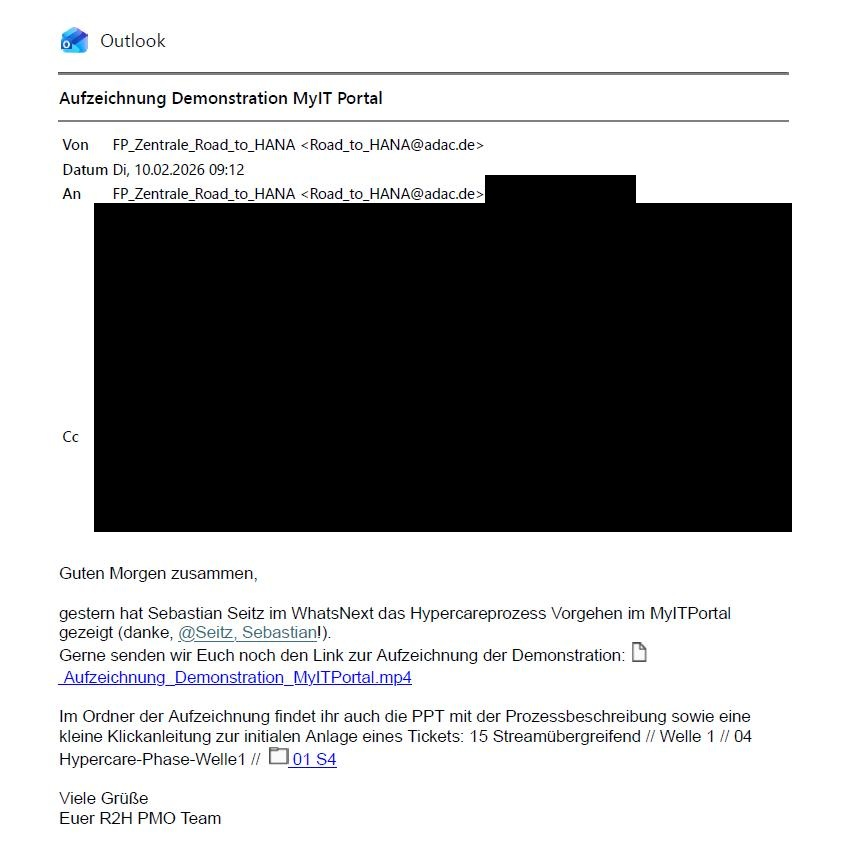
\includegraphics[width=0.99\textwidth]{98_Pictures/MyIt-Schulung.jpg}
    \caption{Programmschulung R2H im MyIT-Portal}
     \label{fig:ProgrammschulungMyIt}
\end{figure}

\begin{figure} [!htbp]
    \centering
    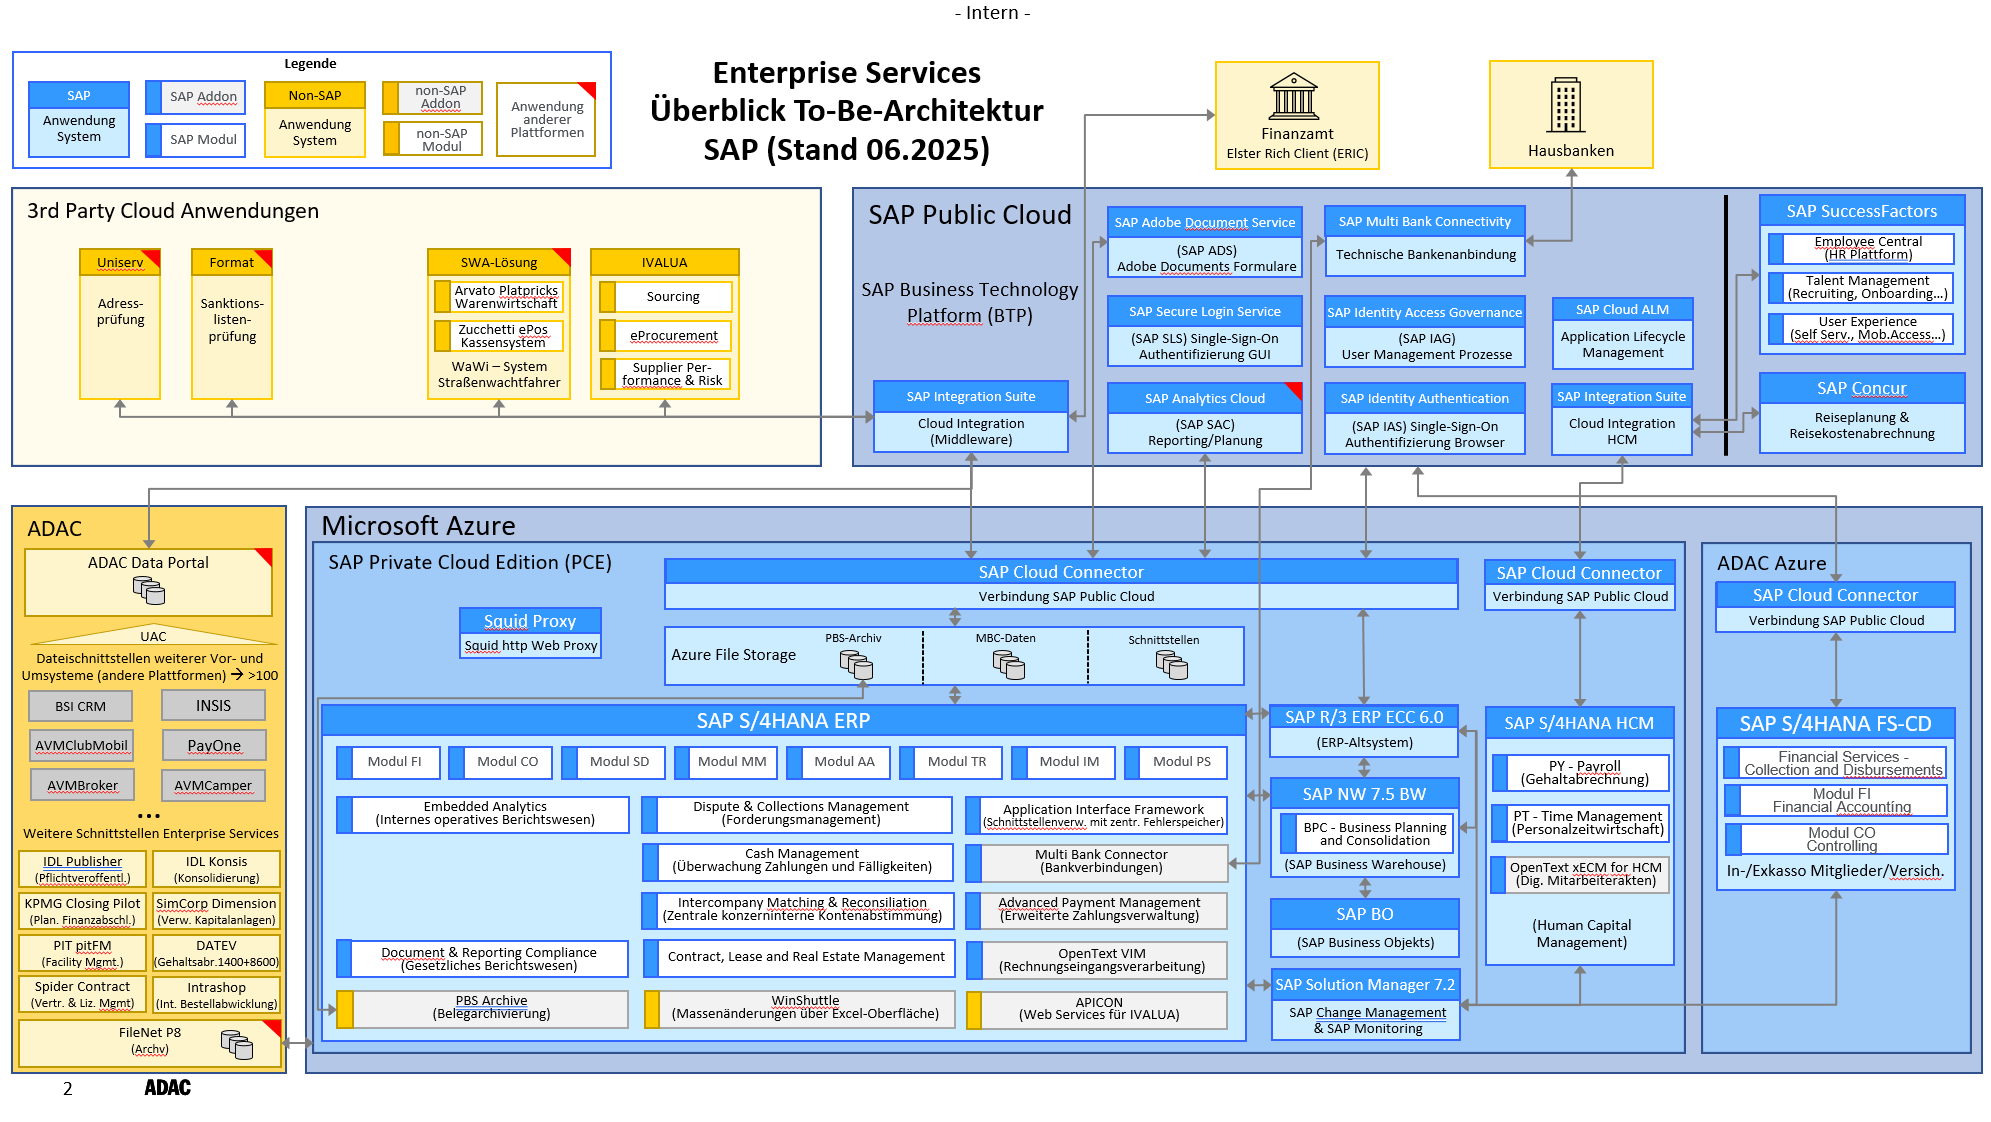
\includegraphics[width=0.99\textwidth]{98_Pictures/R2H_Interfaces_Integration.png}
    \caption{Interfaces und Integrationen von R2H}
     \label{fig:R2HInterfacesIntegration}
\end{figure}

\begin{figure} [!htbp]
    \centering
    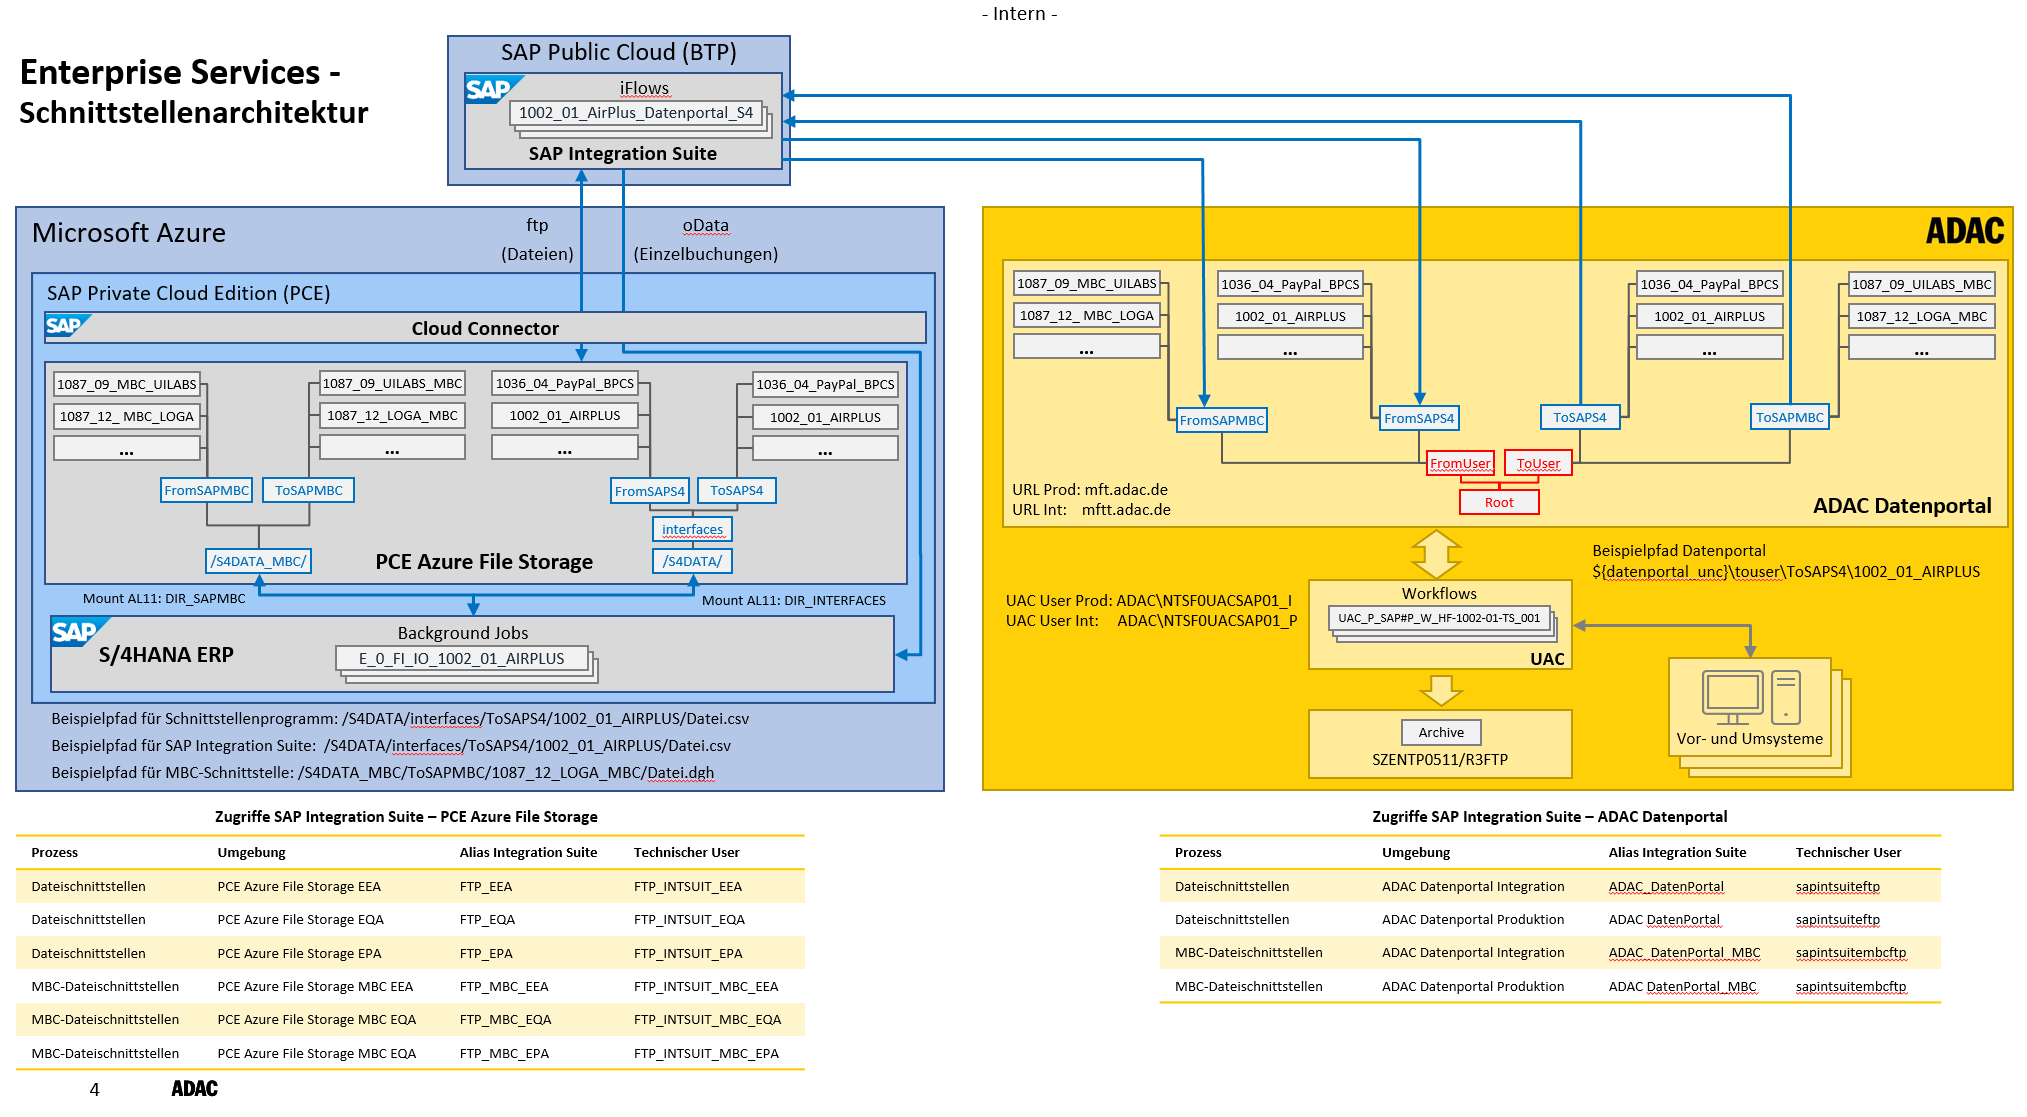
\includegraphics[width=0.99\textwidth]{98_Pictures/R2H_BFA_Detail.png}
    \caption{Detailansicht des implementierten BFA-Modells}
     \label{fig:R2HBFA}
\end{figure}

\clearpage
\newgeometry{top=1cm, bottom=1cm, left=1cm, right=1cm, head=0pt}
\begin{landscape}
\thispagestyle{empty}
\noindent\textit{Report - IPMA Level B}\hfill\textit{Sebastian Seitz}\hfill\textit{IPMA Level B}
\\[-0.9em]
\noindent\rule{\linewidth}{0.1pt}

\begin{figure} [!htbp]
    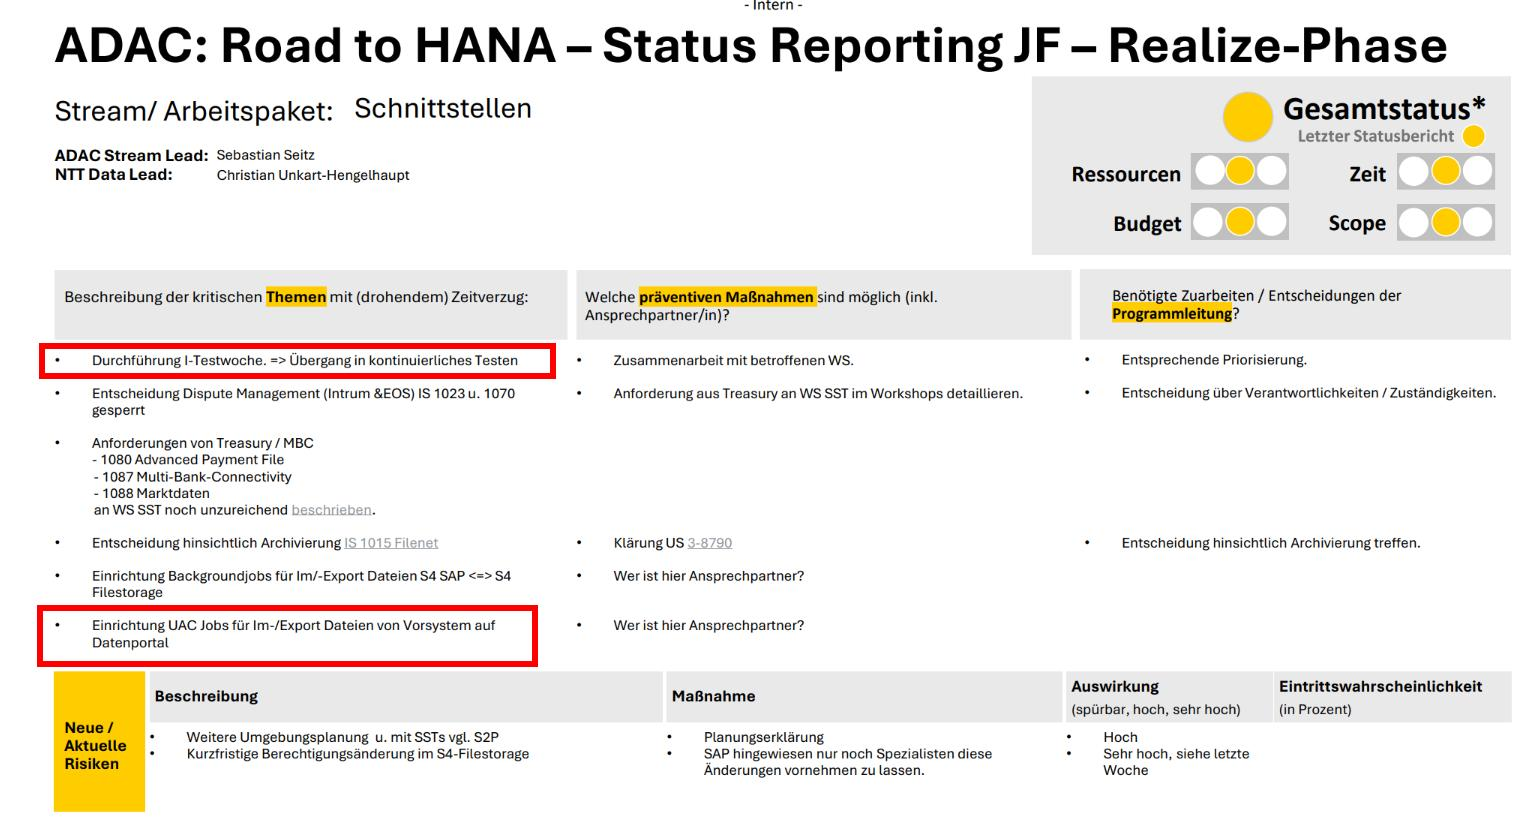
\includegraphics[width=0.99\textwidth]{98_Pictures/260610_StatusFolienSST.jpg}
    \caption{Statusfolie Juni 2025 SST Stand}
     \label{fig:R2HStatusSSTJuni2025}
\end{figure}

\vfill
\par\noindent\rule{\linewidth}{0.1pt}\\[-0.6em]
\noindent\textit{\curse}\hfill\textit{Seite \pagemark{}}
\end{landscape}
\restoregeometry
\clearpage

\begin{figure} [!htbp]
    \centering
    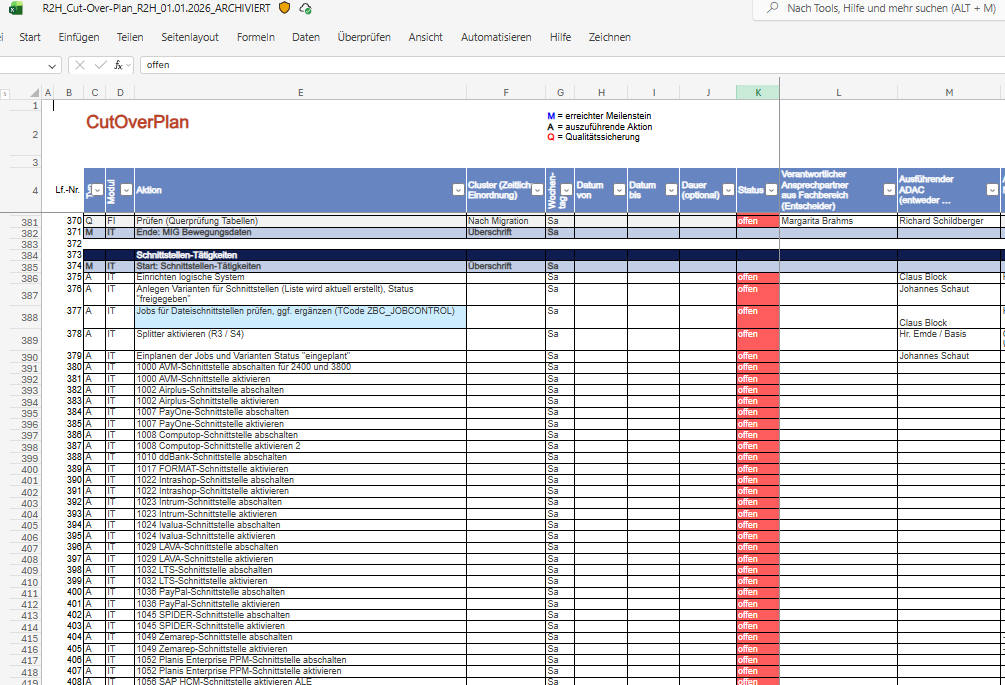
\includegraphics[width=0.99\textwidth]{98_Pictures/CutOverNtt.png}
    \caption{\acrshort{cop} \acrshort{gu} \acrshort{ricefw}}
     \label{fig:CutOverPlanGU}
\end{figure}

\begin{figure} [!htbp]
    \centering
    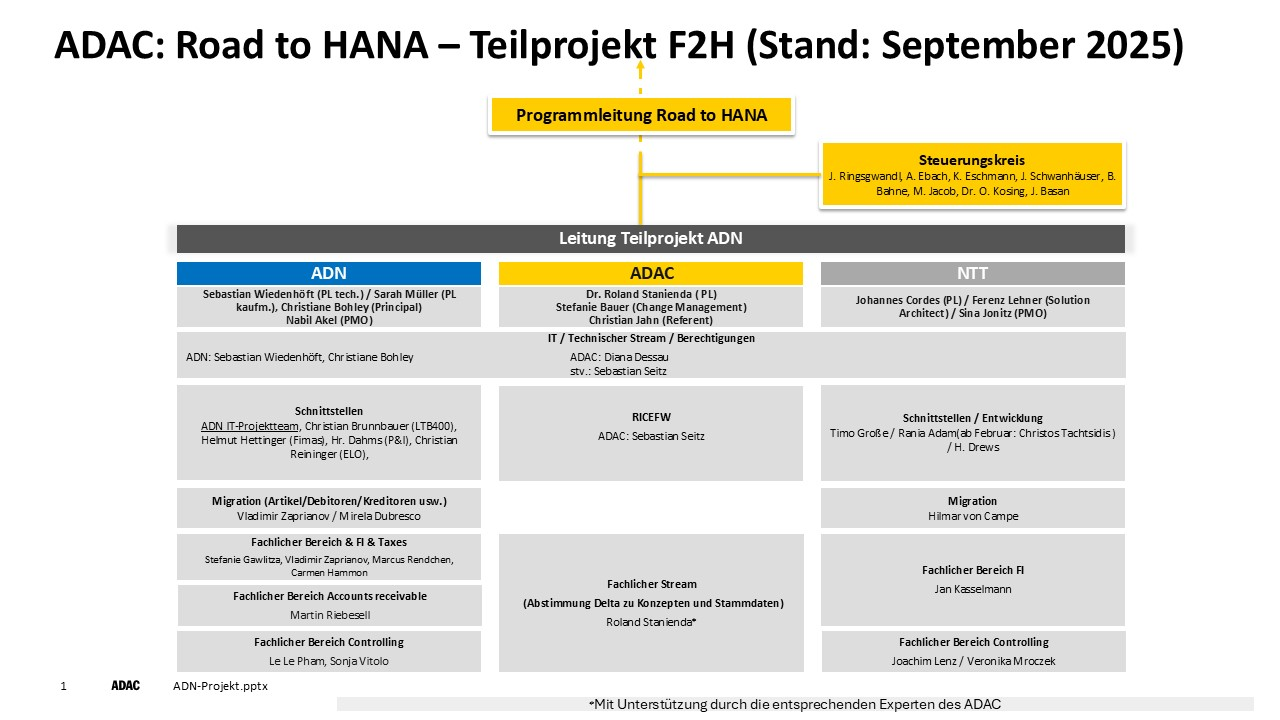
\includegraphics[width=0.99\textwidth]{98_Pictures/F2H_Organigramm_ADN_NTT_ADAC.jpg}
    \caption{Organigramm F2H Projekt}
     \label{fig:F2HOrganigramm}
\end{figure}

\begin{figure} [!htbp]
    \centering
    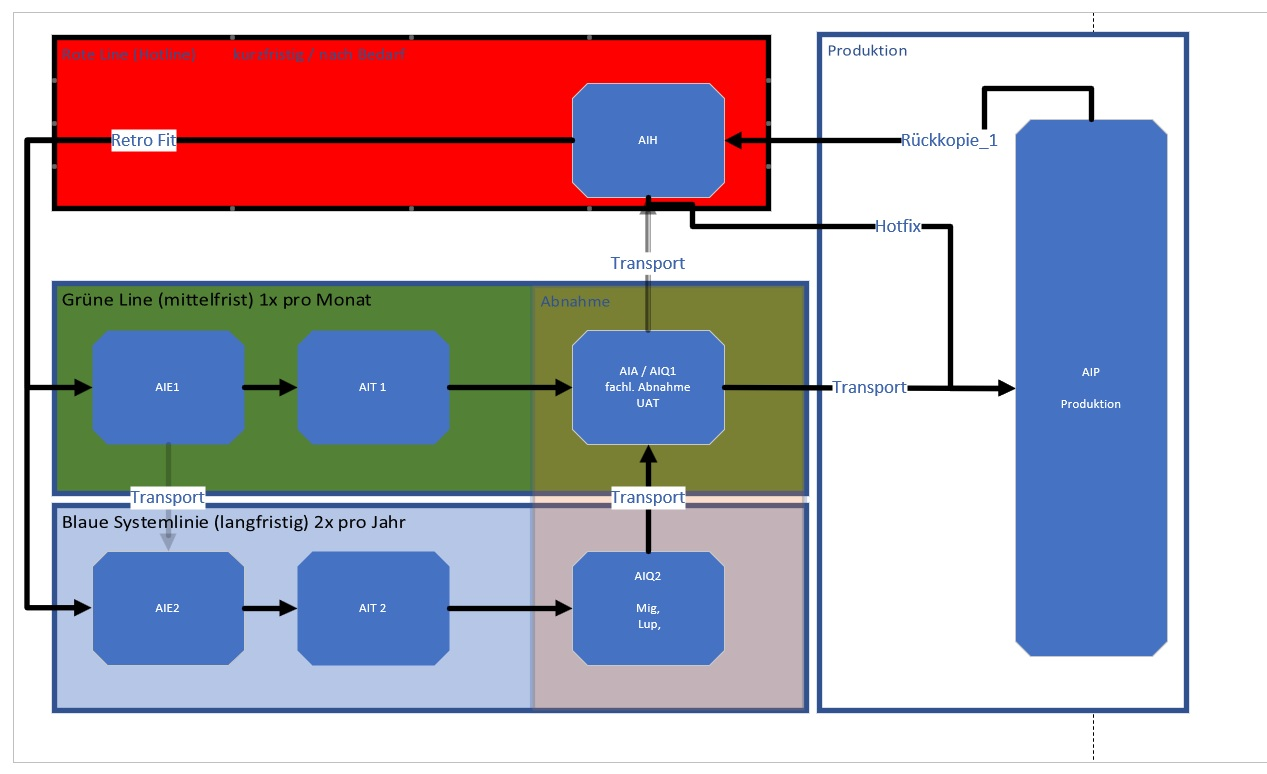
\includegraphics[width=0.99\textwidth]{98_Pictures/SAPUmgebungszielbild.jpg}
    \caption{Zielbild der \acrshort{erp}-SAP-Umgebungslandschaft}
     \label{fig:SAPUmgebungszielbild}
\end{figure}

\noindent
\begin{minipage}[t]{0.49\textwidth}
    \centering
    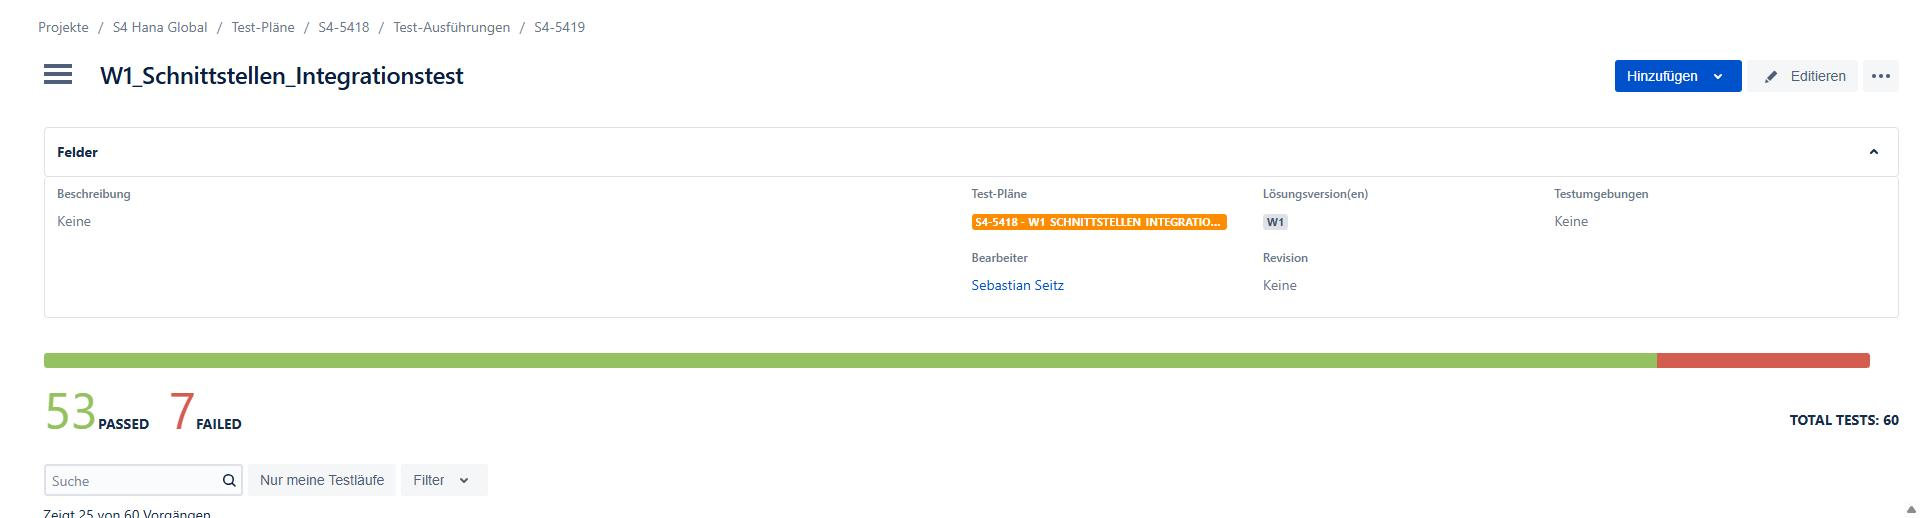
\includegraphics[width=\textwidth]{98_Pictures/TestpläneSST.jpg}
    \captionof{figure}{Testpläne \acrshort{sst}}
    \label{fig:TestpläneSST}
\end{minipage}
\hfill
\begin{minipage}[t]{0.49\textwidth}
    \centering
    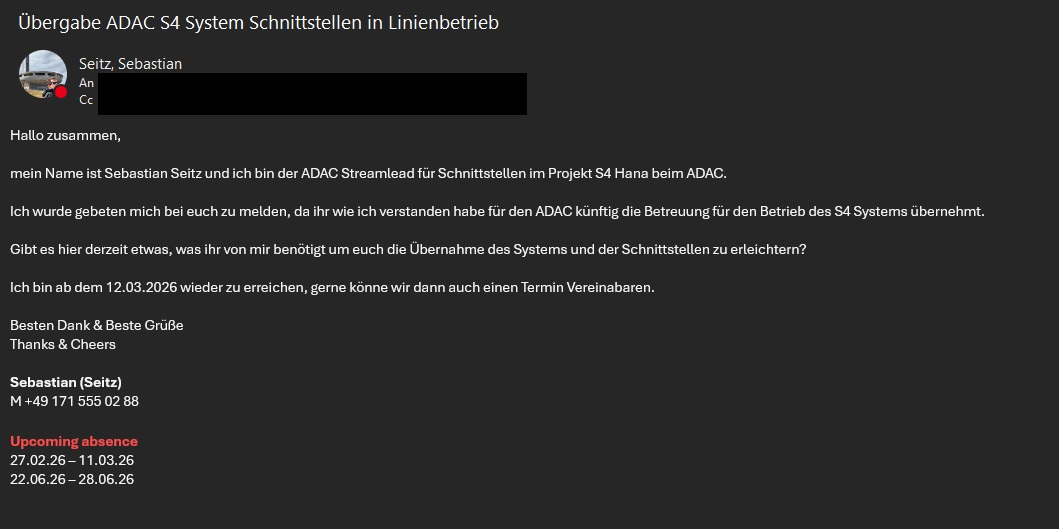
\includegraphics[width=\textwidth]{98_Pictures/InitiierungÜbergabe.jpg}
    \captionof{figure}{Initiierung Betriebsübergabe}
    \label{fig:InitiierungBetriebsübergabe}
\end{minipage}

\begin{figure} [!htbp]
    \centering
    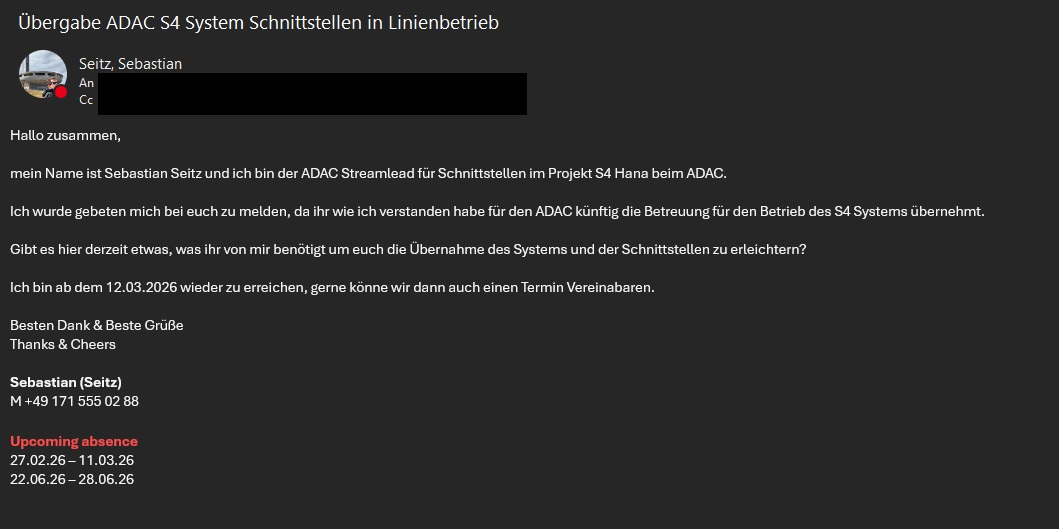
\includegraphics[width=0.99\textwidth]{98_Pictures/InitiierungÜbergabe.jpg}
    \caption{Initiierung und Übergabe}
     \label{fig:InitiierungÜbergabe}
\end{figure}

\begin{figure} [!htbp]
    \centering
    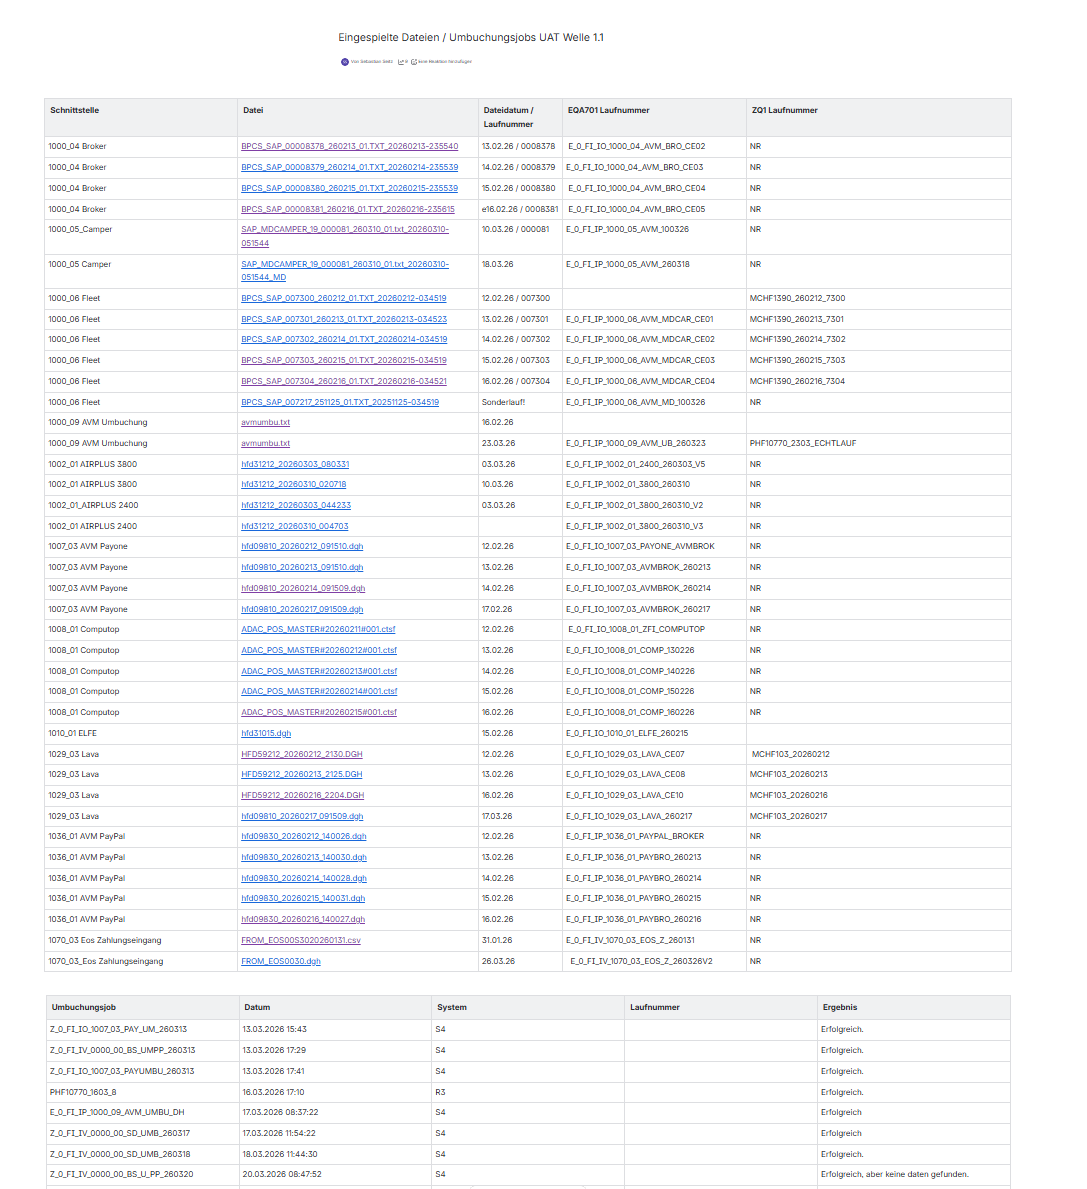
\includegraphics[width=0.99\textwidth]{98_Pictures/UAT_DatenDoku.png}
    \caption{UAT W1.1 Datendokumentation}
     \label{fig:UATDatenDoku}
\end{figure}

\begin{figure} [!htbp]
    \centering
    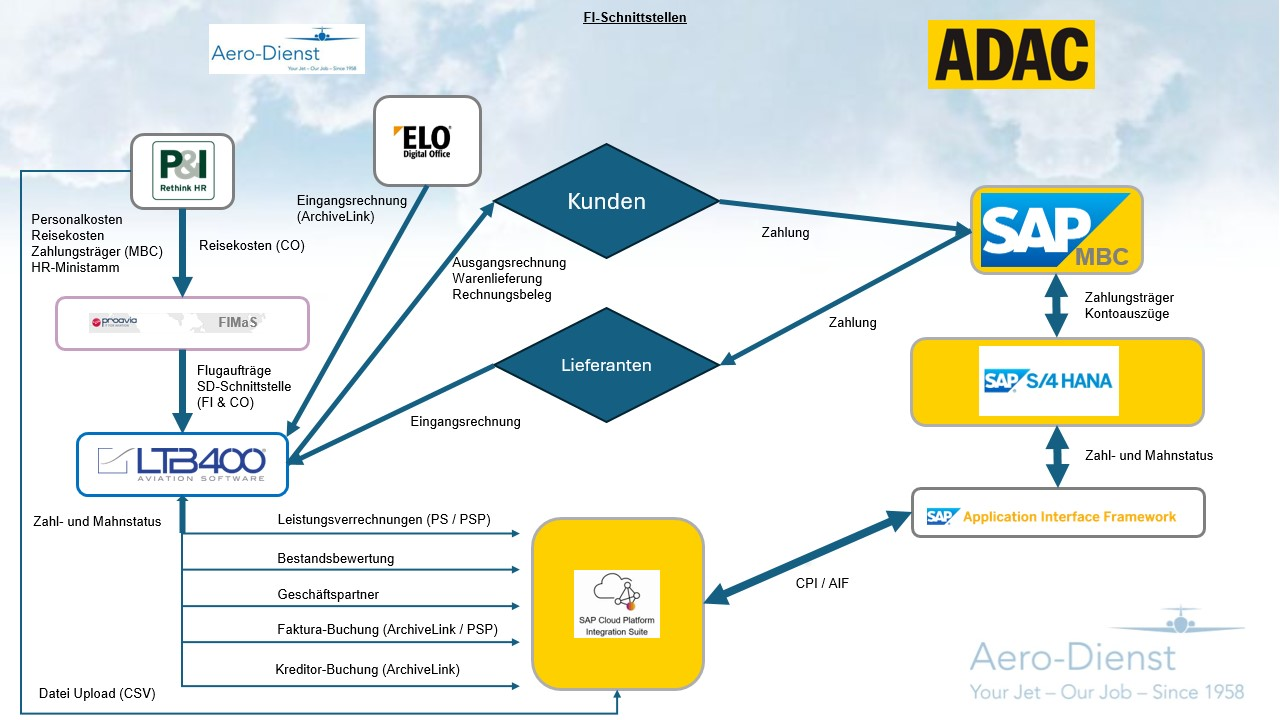
\includegraphics[width=0.99\textwidth]{98_Pictures/ADN_SST_FI.jpg}
    \caption{ADN SST FI Architekturbild}
     \label{fig:ADNSSTFI}
\end{figure}

\begin{figure} [!htbp]
    \centering
    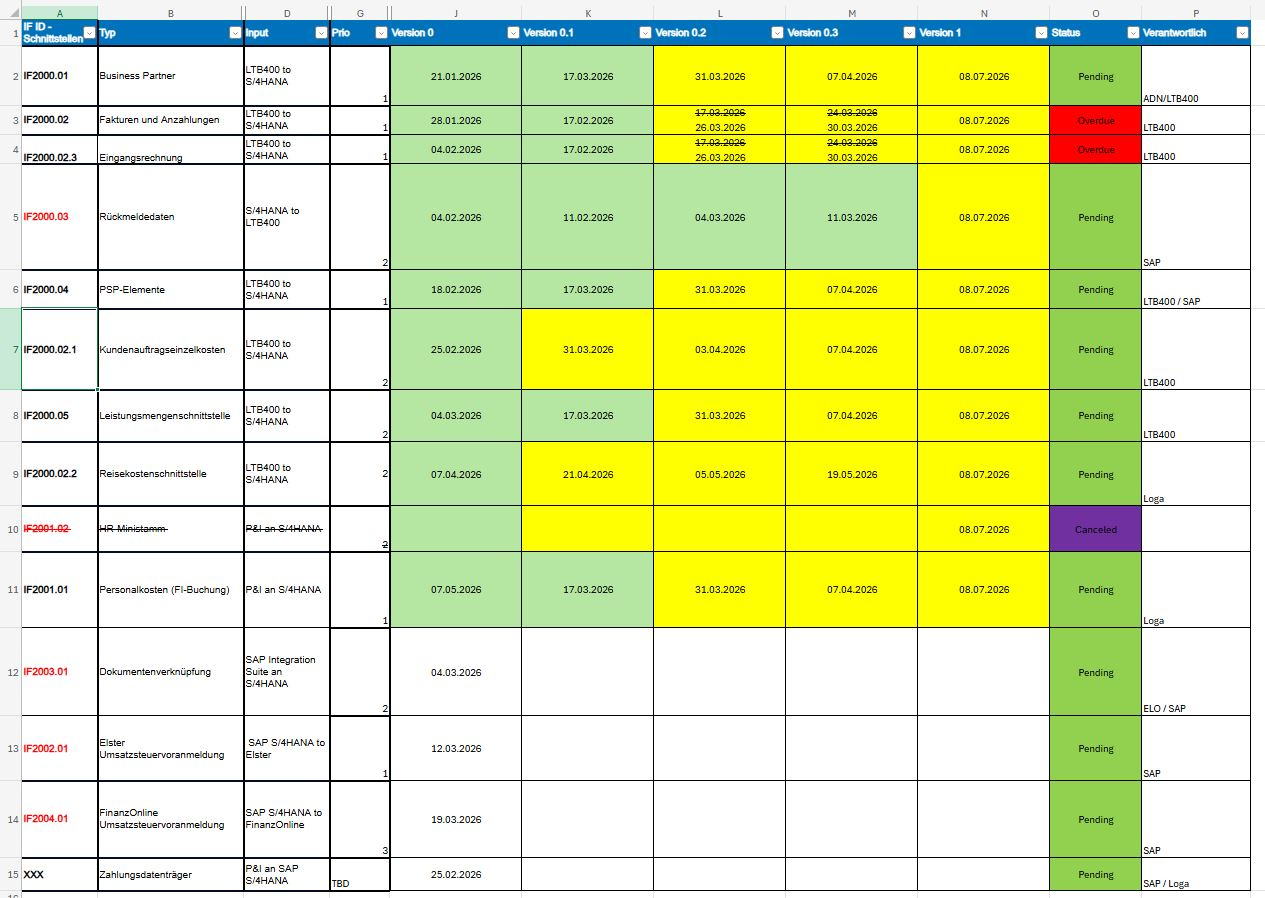
\includegraphics[width=0.99\textwidth]{98_Pictures/VersionsIterationSSTADN.JPG}
    \caption{ADN SST FI Versions- und Iterationsplan}
     \label{fig:VersionsIterationSSTADN}
\end{figure}

\begin{figure} [!htbp]
    \centering
    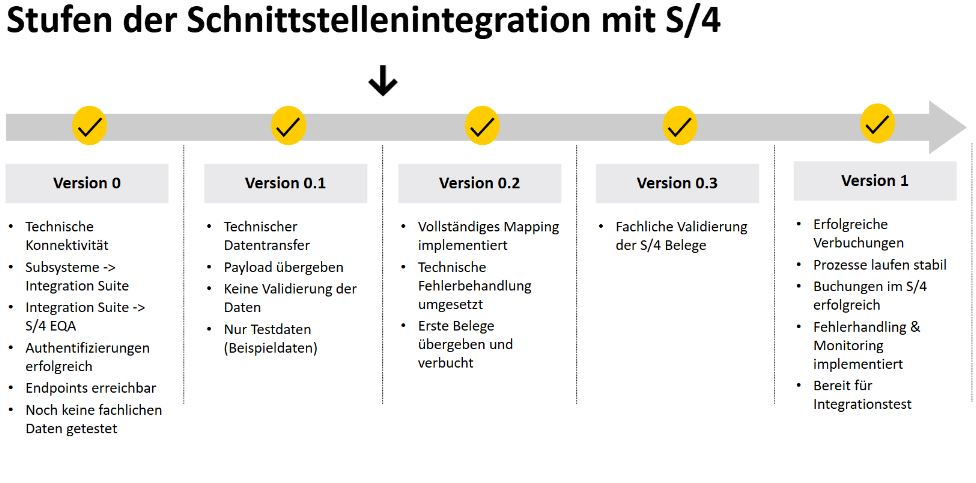
\includegraphics[width=0.99\textwidth]{98_Pictures/StufenIterationErklärung.JPG}
    \caption{ADN SST FI Versions- und Iterationsplan Erklärung}
     \label{fig:StufenIterationErklärung}
\end{figure}

\begin{figure} [!htbp]
    \centering
    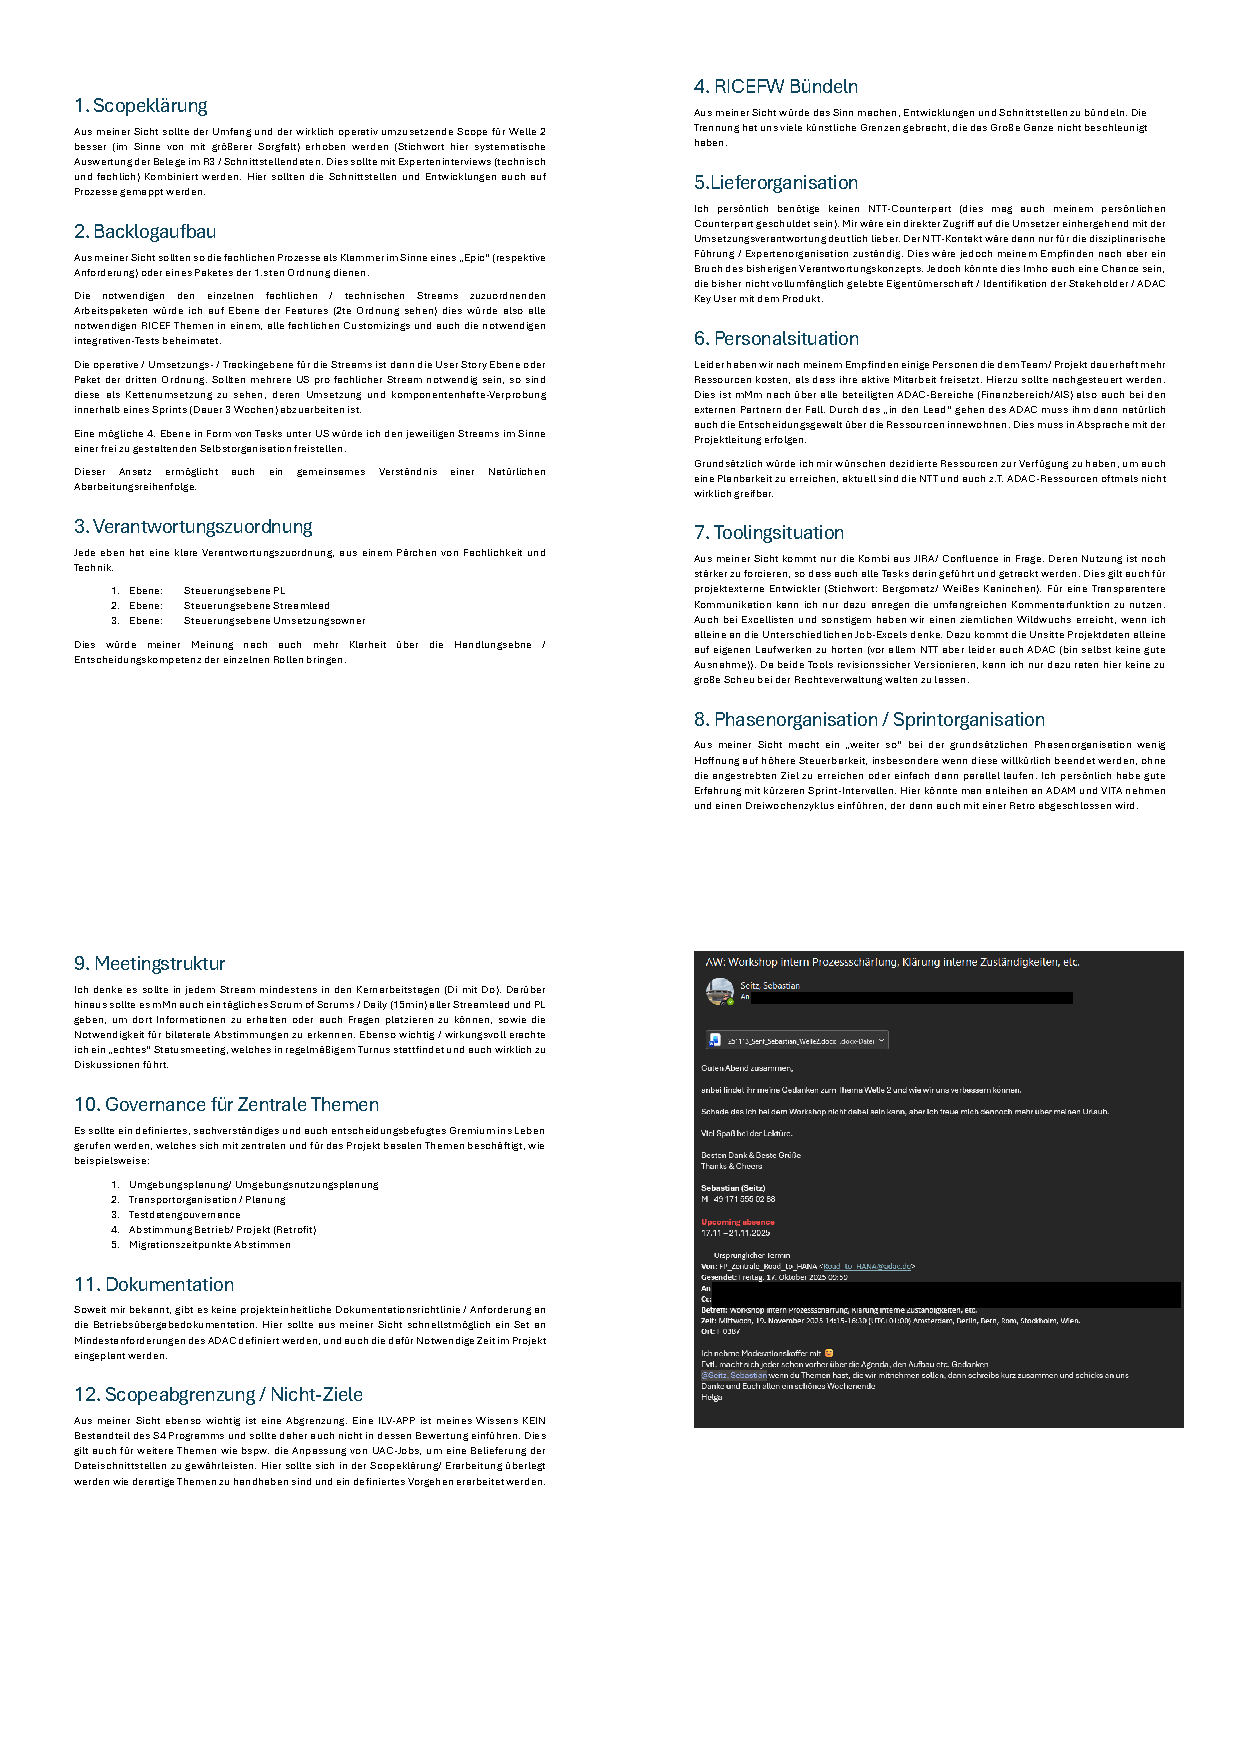
\includegraphics[width=0.99\textwidth]{98_Pictures/251113_Senf_Sebastian_Welle2.pdf}
    \caption{Anregungen W2 und Lessons Learned W1}
     \label{fig:AnregungenW2undLessonsLearnedW1}
\end{figure}

\begin{figure} [!htbp]
    \centering
    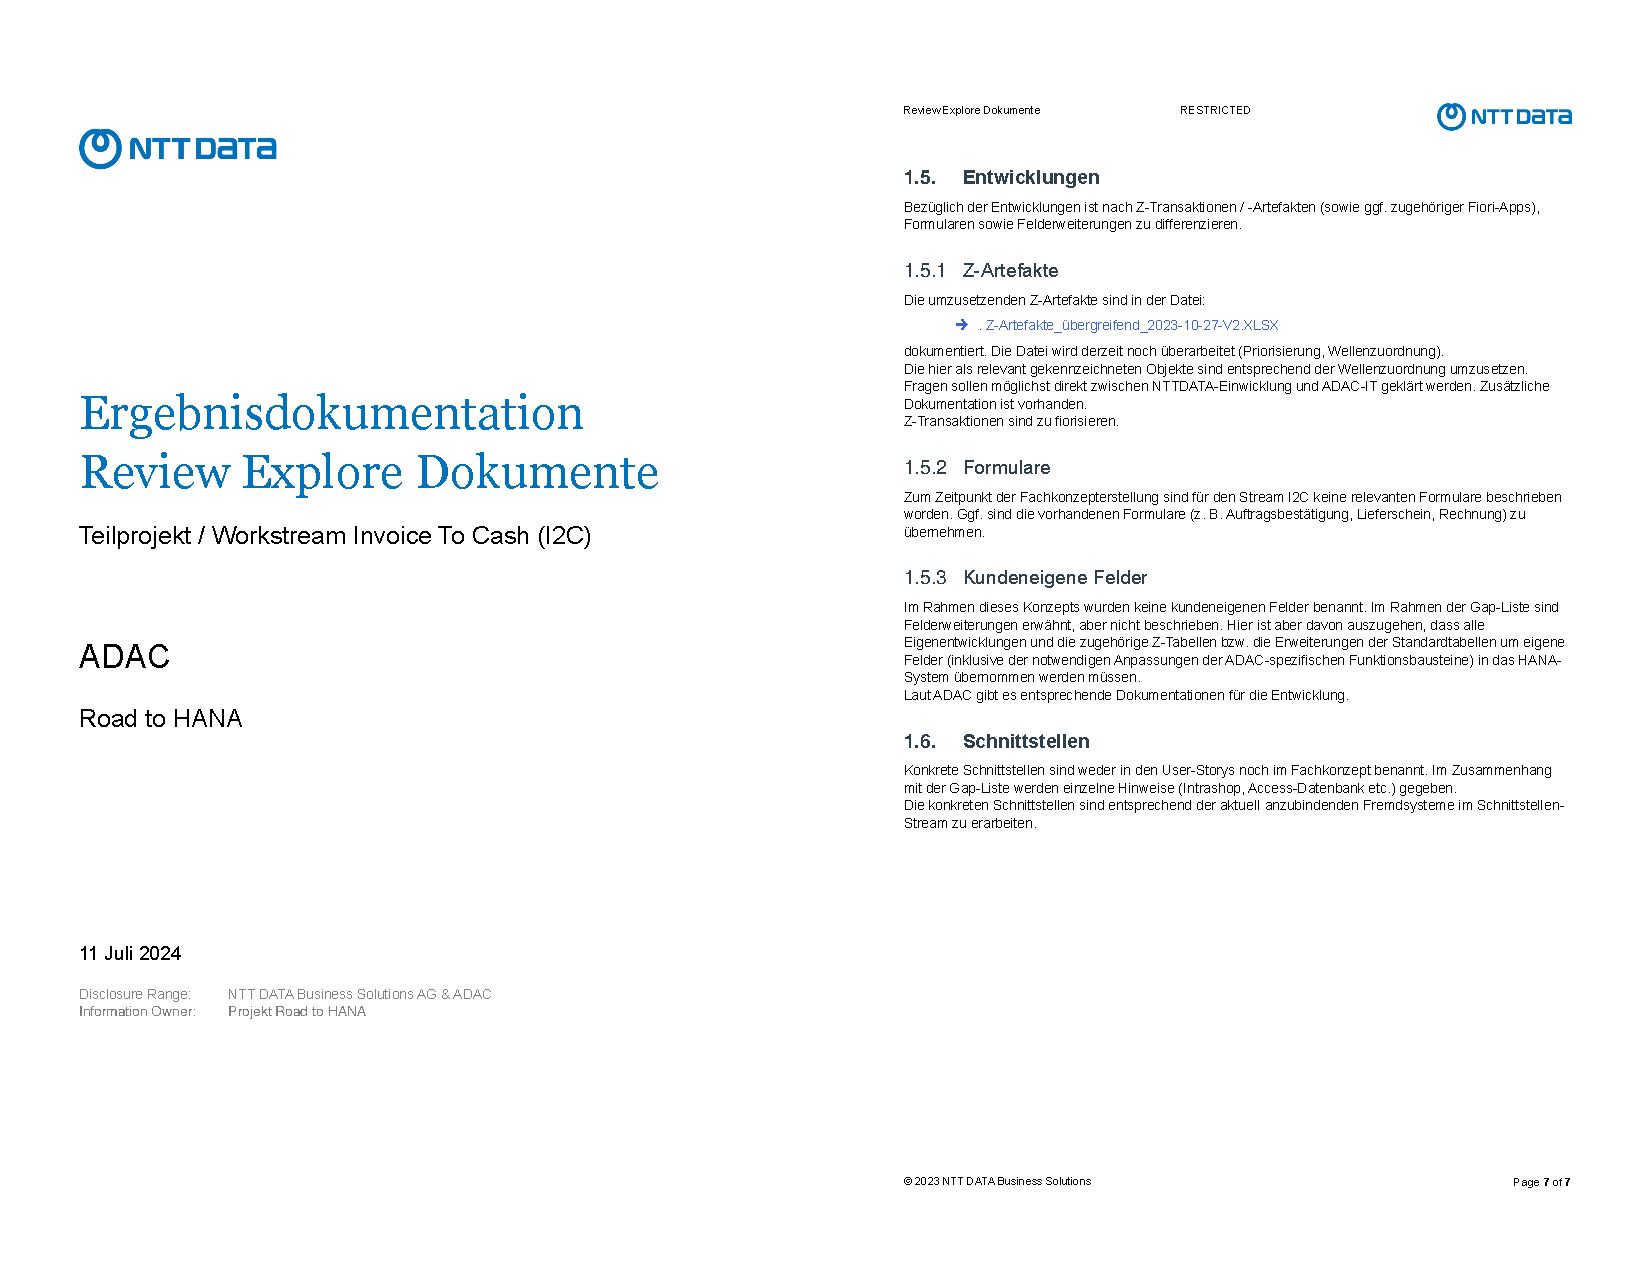
\includegraphics[width=0.99\textwidth]{98_Pictures/R2H_ErgebnisdokumentationStreamI2C.pdf}
    \caption{\acrshort{gu}-Ramp-Up Dokumentation Stream I2C \acrshort{ricefw}+\acrshort{pb}}
     \label{fig:R2HErgebnisdokumentationStreamI2C}
\end{figure}

\newpage

\newpage
\subsection*{Tabellen}
\addcontentsline{toc}{subsection}{Tabellen}

\begin{table}[htpb]
    \begin{tabularx}{\textwidth}{|l|l|X|l|}\rowcolor[HTML]{9B9B9B}
        \textbf{Status} & \textbf{Datum} & \textbf{Beschreibung}                & \textbf{Anzahl} \\ \hline
        Aktualisiert        & 31.03.2026 & Status aktualisiert                  & 2  \\ \hline
        Wartend auf Antwort & 31.03.2026 & Rückmeldung ausstehend               & 3  \\ \hline
        Gelöst              & 31.03.2026 & Vorgang gelöst                       & 4  \\ \hline
        Geschlossen         & 31.03.2026 & Vorgang abgeschlossen                & 62 \\ \hline
        \textbf{Gesamtergebnis} & 31.03.2026 & \textbf{Summe aller Vorgänge}     & \textbf{71} \\ \hline
    \end{tabularx}
    \caption{MyIT Statusübersicht \acrshort{ricefw} ende \acrshort{hypc}}
     \label{tab:statusuebersicht}
\end{table}



\begin{table}
\begin{tabularx}{\textwidth}{|l|l|l|l|l|l|}\rowcolor[HTML]{9B9B9B}
\textbf{\gls{bk}} & \textbf{Firma} & \textbf{Wellle} & \textbf{Ort} & \textbf{Länderschlüssel} & \textbf{Währung} \\ \hline
1000 & ADAC e.V. & 3.0 & München & DE & EUR \\ \hline
1100 & ADAC Luftrettung gGmbH & 4.0 & Weßling & DE & EUR \\ \hline
1200 & ADAC Stift. Gelber Engel & 3.0 & München & DE & EUR \\ \hline
1300 & ADAC Stiftung & 2.0 & München & DE & EUR \\ \hline
1400 & ADAC Customer Service Gmb & 2.0 & München & DE & EUR \\ \hline
1700 & ADAC Motorsport GmbH & 3.0 & München & DE & EUR \\ \hline
1800 & ADAC Digitale Mglst. GmbH & 2.0 & München & DE & EUR \\ \hline
2000 & ADAC SE & 2.0 & München & DE & EUR \\ \hline 
2100 & ADAC Medien und ReiseGmbH & 3.0 & München & DE & EUR \\ \hline
2200 & ADAC Touring GmbH & 3.0 & München & DE & EUR \\ \hline
2300 & ADAC Service GmbH & 3.0 & München & DE & EUR \\ \hline
2400 & ADAC Autovermietung GmbH & 1.1 & München & DE & EUR \\ \hline
2500 & ADAC Telematik GmbH & 3.0 & München & DE & EUR \\ \hline
2600 & ADAC Motorsport GmbH & 3.0 & München & DE & EUR \\ \hline
2700 & ADAC Fahrsicherh. GmbH & 3.0 & München & DE & EUR \\ \hline
2800 & HMS Helicopt.Medical GmbH & 3.0 & München & DE & EUR \\ \hline
2900 & ADAC Finanzdienste GmbH & 2.0 & München & DE & EUR \\ \hline
3000 & ADAC RSR GmbH & 3.0 & München & DE & EUR \\ \hline
3100 & ADAC HEMS Academy GmbH & 3.0 & Weßling & DE & EUR \\ \hline
3200 & PiNCAMP GmbH & 3.0 & München & DE & EUR \\ \hline
3400 & ADAC Aquico GmbH & 2.0 & München & DE & EUR \\ \hline
3500 & Aero-Dienst Verwaltungs G & 3.0 & Nürnberg & DE & EUR \\ \hline
3600 & ADAC TruckService Verwalt & 3.0 & Laichingen & DE & EUR \\ \hline
3700 & ADAC Compliance Service G & 3.0 & München & DE & EUR \\ \hline
3800 & ADAC IT Service GmbH & 1.0 & München & DE & EUR \\ \hline
4000 & ADAC Unterstützungsk.GmbH & 2.0 & München & DE & EUR \\ \hline
4100 & ADAC Stiftung Sport & 2.0 & München & DE & EUR \\ \hline
4200 & ADAC RSB AG \& Co. oHG & 3.0 & München & DE & EUR \\ \hline
4300 & ADAC Tiefg.-Betr. GBR & 3.0 & München & DE & EUR \\ \hline
6000 & ADAC-Rechtsschutz-AG & 3.0 & München & DE & EUR \\ \hline
6100 & ADAC Versicherung AG & 3.0 & München & DE & EUR \\ \hline
6200 & ADAC DTC-Versicherungs AG & 3.0 & München & DE & EUR \\ \hline
6600 & ARISA Assurances S.A. & 3.0 & Luxembourg & LU & EUR \\ \hline
6700 & ARISA Ré S.A., Luxemburg & 3.0 & Luxembourg & LU & EUR \\ \hline
8000 & Aero-Dienst GmbH & 1.3 & Nürnberg & DE & EUR \\ \hline
8100 & ADAC Heliservice GmbH & 3.0 & St. Augustin & DE & EUR \\ \hline
8200 & HMotion GmbH & 3.0 & Gilching & DE & EUR \\ \hline
8300 & Dienstleistungs-Center Ha & 3.0 & Halle & DE & EUR \\ \hline
8500 & ADAC TruckService GmbH \& & 3.0 & Laichingen & DE & EUR \\ \hline
8600 & GKS Gesellschaft für Komm & 3.0 & Passau & DE & EUR \\ \hline
8700 & Car-Port Autotransp. GmbH & 3.0 & Schönkirchen & DE & EUR \\ \hline
9100 & ADAC HEMS und Fachkräfte & 3.0 & München & DE & EUR \\ \hline
9300 & ADAC Service Hellas A.E. & 3.0 & Glyfada & GR & EUR \\ \hline
9400 & ADAC Service Adria d.o.o. & 3.0 & Zagreb & HR & HRK \\ \hline
\end{tabularx}
\caption{Wellenzuordnung der Buchungskreise \gls{r2h} Stand 01.05.2026}
\label{tab:wellenzuordnung}
\end{table}

\label{finalpage}
%\newpage
\end{document}